\documentclass[twoside,openright,numbers,spanish]{ezthesis}
\usepackage{helvet}
%% # Opciones disponibles para el documento #
%%
%% Las opciones con un (*) son las opciones predeterminadas.
%%
%% Modo de compilar:
%%   draft            - borrador con marcas de fecha y sin im'agenes
%%   draftmarks       - borrador con marcas de fecha y con im'agenes
%%   final (*)        - version final de la tesis
%%
%% Tama'no de papel:
%%   letterpaper (*)  - tama'no carta (Am'erica)
%%   a4paper          - tama'no A4    (Europa)
%%
%% Formato de impresi'on:
%%   oneside          - hojas impresas por un solo lado
%%   twoside (*)      - hijas impresas por ambos lados
%%
%% Tama'no de letra:
%%   10pt, 11pt, o 12pt (*)
%%
%% Espaciado entre renglones:
%%   singlespace      - espacio sencillo
%%   onehalfspace (*) - espacio de 1.5
%%   doublespace      - a doble espacio
%%
%% Formato de las referencias bibliogr'aficas:
%%   numbers          - numeradas, p.e. [1]
%%   authoryear (*)   - por autor y a'no, p.e. (Newton, 1997)
%%
%% Opciones adicionales:
%%   spanish         - tesis escrita en espa'nol
%%
%% Desactivar opciones especiales:
%%   nobibtoc   - no incluir la bibiolgraf'ia en el 'Indice general
%%   nofancyhdr - no incluir "fancyhdr" para producir los encabezados
%%   nocolors   - no incluir "xcolor" para producir ligas con colores
%%   nographicx - no incluir "graphicx" para insertar gr'aficos
%%   nonatbib   - no incluir "natbib" para administrar la bibliograf'ia
\parskip=1pt
%% Paquetes adicionales requeridos se pueden agregar tambi'en aqu'i.
%% Por ejemplo:
%\usepackage{subfig}
\usepackage{multirow}
%% # Datos del documento #
%% Nota que los acentos se deben escribir: \'a, \'e, \'i, etc.
%% La letra n con tilde es: \~n.

\author{Milver Felipe Flores Acevedo}
\title{algoritmos y tecn\'icas de generac\'ion de datos de prueba para base de datos basados en idioms}

\usepackage{graphicx} % figuras
\usepackage{subfigure} % subfiguras
%%\usepackage[capposition=top]{floatrow}


\usepackage{algorithm}
\usepackage{algorithmic}

\floatname{algorithm}{Algoritmo}
\renewcommand{\listalgorithmname}{Lista de algoritmos}
\renewcommand{\algorithmicrequire}{\textbf{Entrada:}}
\renewcommand{\algorithmicensure}{\textbf{Salida:}}
\renewcommand{\algorithmicend}{\textbf{fin}}
\renewcommand{\algorithmicif}{\textbf{si}}
\renewcommand{\algorithmicthen}{\textbf{entonces}}
\renewcommand{\algorithmicelse}{\textbf{si no}}
\renewcommand{\algorithmicelsif}{\algorithmicelse,\ \algorithmicif}
\renewcommand{\algorithmicendif}{\algorithmicend\ \algorithmicif}
\renewcommand{\algorithmicfor}{\textbf{para}}
\renewcommand{\algorithmicforall}{\textbf{para todo}}
\renewcommand{\algorithmicdo}{\textbf{hacer}}
\renewcommand{\algorithmicendfor}{\algorithmicend\ \algorithmicfor}
\renewcommand{\algorithmicwhile}{\textbf{mientras}}
\renewcommand{\algorithmicendwhile}{\algorithmicend\ \algorithmicwhile}
\renewcommand{\algorithmicloop}{\textbf{repetir}}
\renewcommand{\algorithmicendloop}{\algorithmicend\ \algorithmicloop}
\renewcommand{\algorithmicrepeat}{\textbf{repetir}}
\renewcommand{\algorithmicuntil}{\textbf{hasta que}}
\renewcommand{\algorithmicprint}{\textbf{imprimir}} 
\renewcommand{\algorithmicreturn}{\textbf{devolver}} 
\renewcommand{\algorithmictrue}{\textbf{cierto }} 
\renewcommand{\algorithmicfalse}{\textbf{falso }} 


\usepackage{listings}
%\newcaptionname{spanish}{\lstlistingname}{Listado}
 
\usepackage{listings}
\usepackage{color}
\usepackage{lettrine}
\usepackage{booktabs}
\usepackage{multirow}
\usepackage{lscape} %para landscape
\usepackage{caption}
\usepackage{capt-of}

\usepackage{blindtext}
\usepackage{enumitem}

\usepackage[font=scriptsize, textfont=rm,labelfont={sf,bf}, margin=0.5cm]{caption}
\usepackage{mwe}

\usepackage{natbib}
\usepackage{adjustbox}

\definecolor{codegreen}{rgb}{0,0.6,0}
\definecolor{codegray}{rgb}{0.5,0.5,0.5}
\definecolor{codepurple}{rgb}{0.58,0,0.82}
\definecolor{backcolour}{rgb}{0.99,0.99,0.99}
 
\lstdefinestyle{codeStyle}{
    backgroundcolor=\color{backcolour},   
    commentstyle=\color{codegreen},
    keywordstyle=\color{blue},
    numberstyle=\tiny\color{black},
    stringstyle=\color{magenta},
    basicstyle={\ttfamily\singlespacing\footnotesize},
    breakatwhitespace=false,         
    breaklines=true,                 
    captionpos=b,                    
    keepspaces=true,                 
    numbers=left,                    
    numbersep=5pt,                  
    showspaces=false,                
    showstringspaces=false,
    showtabs=false,                  
    tabsize=1,
}
%%\captionsetup[lstlisting]{position=bottom}
\lstset{style=codeStyle}


\degree{ingenieria de sistemas}
\supervisor{juan marcelo flores soliz}
\institution{Universidad Mayor de San Sim\'on}
\faculty{Facultad de Ciencias y Tecnolog\'ia}
\department{Carrera en Licenciatura de Ingenieria de Sistemas}

%% # M'argenes del documento #
%% 
%% Quitar el comentario en la siguiente linea para austar los m'argenes del
%% documento. Leer la documentaci'on de "geometry" para m'as informaci'on.

\geometry{top=20mm,bottom=20mm,inner=30mm,outer=20mm}
\setcounter{secnumdepth}{3} % para que ponga 1.1.1.1..
\setcounter{tocdepth}{4} % para que añadir las secciones en el índice...

\renewcommand{\lstlistingname}{Codigo}
%% El siguiente comando agrega ligas activas en el documento para las
%% referencias cruzadas y citas bibliogr'aficas. Tiene que ser *la 'ultima*
%% instrucci'on antes de \begin{document}.
\hyperlinking

\begin{document}

%%\thispagestyle{empty}
%%\setcounter{page}{0}
%% En esta secci'on se describe la estructura del documento de la tesis.
%% Consulta los reglamentos de tu universidad para determinar el orden
%% y la cantidad de secciones que debes de incluir.
% display page numbers in the headings. Start with roman numerals %
%% # Portada de la tesis #
%% Mirar el archivo "titlepage.tex" para los detalles.
%% ## Construye tu propia portada ##
%% 
%% Una portada se conforma por una secuencia de "Blocks" que incluyen
%% piezas individuales de informaci'on. Un "Block" puede incluir, por
%% ejemplo, el t'itulo del documento, una im'agen (logotipo de la universidad),
%% el nombre del autor, nombre del supervisor, u cualquier otra pieza de
%% informaci'on.
%%
%% Cada "Block" aparece centrado horizontalmente en la p'agina y,
%% verticalmente, todos los "Blocks" se distruyen de manera uniforme 
%% a lo largo de p'agina.
%%
%% Nota tambi'en que, dentro de un mismo "Block" se pueden cortar
%% lineas usando el comando \\
%%
%% El tama'no del texto dentro de un "Block" se puede modificar usando uno de
%% los comandos:
%%   \small      \LARGE
%%   \large      \huge
%%   \Large      \Huge
%%
%% Y el tipo de letra se puede modificar usando:
%%   \bfseries - negritas
%%   \itshape  - it'alicas
%%   \scshape  - small caps
%%   \slshape  - slanted
%%   \sffamily - sans serif
%%
%% Para producir plantillas generales, la informaci'on que ha sido inclu'ida
%% en el archivo principal "tesis.tex" se puede accesar aqu'i usando:
%%   \insertauthor
%%   \inserttitle
%%   \insertsupervisor
%%   \insertinstitution
%%   \insertdegree
%%   \insertfaculty
%%   \insertdepartment
%%   \insertsubmitdate

\begin{titlepage}
  \TitleBlock{\scshape\insertinstitution}
  \TitleBlock[\bigskip]{\scshape\insertfaculty}
  \TitleBlock{\Huge\scshape\inserttitle}
  \TitleBlock{\scshape
    Tesis presentada por \insertauthor \\
    para obtener el grado de \insertdegree\\
    Tutorado por \insertsupervisor}
  \TitleBlock{\insertsubmitdate}
  \TitleBlock[\bigskip]{\insertdepartment}
\end{titlepage}

%% Nota 1:
%% Se puede agregar un escudo o logotipo en un "Block" como:
%%   \TitleBlock{\includegraphics[height=4cm]{escudo_uni}}
%% y teniendo un archivo "escudo_uni.pdf", "escudo_uni.png" o "escudo_uni.jpg"
%% en alg'un lugar donde LaTeX lo pueda encontrar.

%% Nota 2:
%% Normalmente, el espacio entre "Blocks" se extiende de modo que el
%% contenido se reparte uniformemente sobre toda la p'agina. Este
%% comportamiento se puede modificar para mantener fijo, por ejemplo, el
%% espacio entre un par de "Blocks". Escribiendo:
%%   \TitleBlock{Bloque 1}
%%   \TitleBlock[\bigskip]{Bloque2}
%% se deja un espacio "grande" y de tama~no fijo entre el bloque 1 y 2.
%% Adem'as de \bigskip est'an tambi'en \smallskip y \medskip. Si necesitas
%% aun m'as control puedes usar tambi'en, por ejemplo, \vspace*{2cm}.



%% # Prefacios #
%% Por cada prefacio (p.e. agradecimientos, resumen, etc.) crear
%% un nuevo archivo e incluirlo aqu'i.
%% Para m'as detalles y un ejemplo mirar el archivo "gracias.tex".
%% Las secciones del "prefacio" inician con el comando \prefacesection{T'itulo}
%% Este tipo de secciones *no* van numeradas, pero s'i aparecen en el 'indice.
%%
%% Si quieres agregar una secci'on que no vaya n'umerada y que *tampoco*
%% aparesca en el 'indice, usa entonces el comando \chapter*{T'itulo}
%%
%% Recuerda que aqu'i ya puedes escribir acentos como: 'a, 'e, 'i, etc.
%% La letra n con tilde es: 'n.

\prefacesection{Agradecimientos}
Este trabajo se la dedico al creador de todas las cosas qui\'en supo guiarme por el buen
camino, darme fuerzas para seguir adelante y no desmayar en los
problemas que se presentaban, ense\~n\'andome a encarar las
adversidades sin perder nunca la dignidad ni desfallecer en el
intento.

A mi familia quienes por ellos soy lo que soy.
Para mis padres por su apoyo, consejos, comprensi\'on, amor, ayuda
en los momentos dif\'iciles, y por ayudarme con los recursos necesarios
para estudiar. Me han dado todo lo que soy como persona, mis
valores, mis principios, mi car\'acter, mi empe\~no, mi perseverancia,
mi coraje para conseguir mis objetivos.
A mis hermanas por estar siempre presentes, acompa\~na\'ndome para
poderme realizar. 


A mi tutor por la orientaci\'on y ayuda que me brind\'o para la realizaci\'on de este trabajo, por su apoyo y amistad que me permitieron aprender mucho m\'as que lo estudiado en el proyecto.
%% Por si alguien tiene curiosidad, este "simp'atico" agradecimiento est'a
%% tomado de la "Tesis de Lydia Chalmers" basada en el universo del programa
%% de televisi'on Buffy, la Cazadora de Vampiros.
%% http://www.buffy-cazavampiros.com/Spiketesis/tesis.inicio.htm


%%include indice
%% # 'Indices y listas de contenido #
%% Quitar los comentarios en las lineas siguientes para obtener listas de
%% figuras y cuadros/tablas.
\cleardoublepage
\tableofcontents
\cleardoublepage
\listoffigures
\cleardoublepage
\listoftables
\cleardoublepage
%% # Cap'itulos #
%% Por cada cap'itulo hay que crear un nuevo archivo e incluirlo aqu'i.
%% Mirar el archivo "intro.tex" para un ejemplo y recomendaciones para
%% escribir.
%\chapter*{Resumen}
\thispagestyle{empty}
\renewcommand{\footrulewidth}{0.0pt}% linea footer
En el desarrollo de software que implica el uso de base de datos, es bastante com\'un requerir realizar pruebas para conocer el comportamiento del software conjuntamente con la base de datos, para lo cual es necesario tener la base de datos poblada con datos de prueba similar cuando el software este en un entorno de producci\'on. 

Si bien se tiene claro que es necesario tener la base de datos poblada, no resulta ser tan sencillo poblar con datos de prueba por razones como resulta ser tedioso debido a que no siempre se tiene en mente lo que se quiere, tener en mente nombres de las tablas y quien referencia a quien, por lo cual normalmente se acostumbra a insertar pocos datos datos de prueba, como resultado deja la incertedumbre de como vaya ser el comportamiento de las consultas que se realiza. Este trabajo se presenta una propuesta algoritmos y t\'ecnicas  que ayudan de alguna manera el llenado de datos de prueba en una base de datos basados, tomando encuenta las referencias compuestas comunes en modelos ER basados en Idioms, ademas se presenta algoritmos para obtener el orden correcto en que deben ser llenado con datos de prueba las tablas de una base de datos para lo cual se tiene algoritmos que generan datos segun el tipo dato, para el caso de las llaves foraneas se ofrece mecanismos que autogeneran apartir de la tabla al que referencia para evitar la inconsistencia de datos, otro caso importante es el tipo de dato binario en este proyecto se opta por trabajar con Postgresql que ofrece su tipo de dato \texttt{bytea} para almacenar archivos en la base de datos como demostracion de todo lo desarrollado se presenta un prototipo que genera datos directamente a la base de datos con la opcion de crear un archivo con extension sql siempre que la base de datos no tenga tipo de datos binarios.

\chapter*{Resumen}
\thispagestyle{empty}
\renewcommand{\footrulewidth}{0.0pt}% linea footer
En el desarrollo de software que implica el uso de base de datos, es bastante com\'un requerir realizar pruebas para conocer el comportamiento del software conjuntamente con la base de datos, para lo cual es necesario tener la base de datos poblada con datos de prueba similar cuando el software este en un entorno de producci\'on. 

Si bien se tiene claro que es necesario tener la base de datos poblada, no resulta ser tan sencillo poblar con datos de prueba por razones como resulta ser tedioso debido a que no siempre se tiene en mente lo que se quiere, tener en mente nombres de las tablas y quien referencia a quien, por lo cual normalmente se acostumbra a insertar pocos datos datos de prueba, como resultado deja la incertedumbre de como vaya ser el comportamiento de las consultas que se realiza. Este trabajo se presenta una propuesta algoritmos y t\'ecnicas  que ayudan de alguna manera el llenado de datos de prueba en una base de datos basados, tomando encuenta las referencias compuestas comunes en modelos ER basados en Idioms, ademas se presenta algoritmos para obtener el orden correcto en que deben ser llenado con datos de prueba las tablas de una base de datos para lo cual se tiene algoritmos que generan datos segun el tipo dato, para el caso de las llaves foraneas se ofrece mecanismos que autogeneran apartir de la tabla al que referencia para evitar la inconsistencia de datos, otro caso importante es el tipo de dato binario en este proyecto se opta por trabajar con Postgresql que ofrece su tipo de dato \texttt{bytea} para almacenar archivos en la base de datos como demostracion de todo lo desarrollado se presenta un prototipo que genera datos directamente a la base de datos con la opcion de crear un archivo con extension sql siempre que la base de datos no tenga tipo de datos binarios.

%\include{introduccion}
%% Los cap'itulos inician con \chapter{T'itulo}, estos aparecen numerados y
%% se incluyen en el 'indice general.
%%
%% Recuerda que aqu'i ya puedes escribir acentos como: 'a, 'e, 'i, etc.
%% La letra n con tilde es: 'n.

\chapter{Introducci'on}

Cuando se est\'a desarrollando software que hacen  uso de una bases de datos, que est\'a en gran parte de las aplicaciones. Es com\'un tener la necesidad de realizar pruebas sobre la base de datos, para verificar si los datos se est\'an gestionando de la manera correcta o verificar la eficiencia  de las consultas, para esto se insertan datos de prueba haciendo uso de comandos del Lenguaje de definici\'on de datos \texttt{(DDL)} \cite{ddl}.Otra manera es hacerlo por una interfaz gr\'afica dependiendo del sistema gestor de base de datos, entre las mas usadas tenemos a:
\begin{itemize}
\item \textbf{Postgresql}: PgAdmin.
\item \textbf{MySQL}: PhpMyAdmin, MySQL Workbench.
\item \textbf{SQLServer}: .
\end{itemize}
Los que trabajan con base de datos llenaron datos de prueba de esta manera en alg\'un momento o siguen con los mismos m\'etodos.

Insertar datos de prueba en una base de datos de forma manual sea por interfaz gr\'afica o por una interfaz de texto como ser la consola, no suele ser tan agradable porque: conlleva mucho tiempo de trabajo; no siempre se tiene en mente lo que se quiere etc. Por lo que normalmente se insertan pocos datos de prueba para ver el comportamiento de las consultas que se realizan en el software. 

Una aplicaci\'on en un entorno de producci\'on de seguro no lleva pocos datos, al contrario llegan almacenar gigabytes de informaci'on.

El problema surge ah\'i, porque no es lo mismo hacer pruebas con cien datos que con cien mil datos o mas, si bien una consulta funciona de manera correcta con los pocos datos, es diferente el comportamiento con una poblaci'on de datos mas grande, puede que las consultas no funcionen de forma correcta o esta son muy lentas. Un error com'un en principiantes es realizar un \texttt{SELECT * FROM tabla} que de seguro no tendr\'ia problemas con los pocos datos, sin embargo en el entorno de producci'on es catastr\'ofico. 

Sin duda es un problema a considerarse en el desarrollo de software, sobre todo cuando no se realizan pruebas a una base de datos, dej\'andonos incertidumbres sobre su comportamiento con cantidades de datos que podr\'ia tener cuando el software ya est\'e en un entorno producci\'on.
\section{Aplicaciones generadores de datos de prueba para base de datos}
Para los que son nuevos en el mundo de base de datos es normal desconocer sobre herramientas que facilitan la tarea, y optan en llenar de forma manual una base de datos, que resulta ser tedioso y puede llegar a no gustar ser responsable de la parte de la base de datos, si a principios de la aparici'on de la base de datos no se contaba con herramientas de apoyo en esta \'area, hoy en d\'ia existen herramientas que automatizan procesos como el llenado de datos de prueba en cantidades grandes sobre una base de datos ya existente. 

Entre las herramientas para la generaci\'on de datos de prueba para base de datos, se puede mencionar a Datanamic Data Generator MultiDB perteneciente a Datanamic \cite{datanamic}, Generatedata para mysql de c\'odigo abierto con licencia GNU \cite{generatedata}, EMS Data Generator for MySQL de la l\'inea de EMS y EMS Data Generator for PostgreSQL tambi\'en de la l\'inea de EMS \cite{emsdatagenerator} y MyDatagen \cite{mydatagen}, son algunas que podemos mencionar lo cual no significa que sean las \'unicas, con estas herramientas podemos realizar el poblado de datos para su posterior realizaci\'on de pruebas.

De las herramientas el mas destacado es Datanamic, por la forma en como permite configurarlo. En la p\'agina oficial \cite{datanamic} estan disponibles para MySql, PostgreSQL, Oracle y otros. En el caso de Datanamic para PostgreSQL es una de las  m\'as destacables entre las mencionadas ,donde se puede ver opciones de generar datos lo primero es escoger una base de datos existente en otra base de datos y lo que hace el software es reconocer caracter\'isticas de la base de datos, con sus respectivos tipo de datos y por defecto presenta de generar cien registros, con la libertad de configurar a gusto adem\'as da la opci\'on de escoger la fuente de datos que se har\'a uso, a partir de una lista, otro es obtener datos como nombres por ejemplo a partir de un archivo, y poder seleccionar y escoger si ser\'a aleatoriamente o una forma secuencial, si ser\'a \'unico o si se repetir\'a esto dependiendo de c\'omo se quiere llenar datos.

De las otras herramientas mencionadas tienen una similitud en el manejo y en c\'omo se realiza el llenado de los datos, a diferencia de Generatedata que es una herramienta libre y de c\'odigo abierto escrita en JavaScript, PHP y MySQL. Que permite generar de una forma r'apida grandes vol\'umenes de datos personalizados en una variedad de formatos, para su uso en pruebas de software, rellenar bases de datos, etc. Los desarrolladores pueden escribir sus propios tipos de datos para generar nuevos tipos de datos aleatorios e incluso personalizar los tipos de exportaci\'on, Para las personas interesadas en la generaci\'on de datos de localizaci\'on geogr\'afica, se pueden a\~nadir nuevos complementos para proporcionar nombres de regiones (estados, provincias, territorios, etc.), nombres de ciudades y formatos de c\'odigos postales para su pa\'is, todo esto porque es libre de c\'odigo abierto, donde podemos observar que los datos a llenar a una base de datos los extrae de su propia base de datos que incluye Generatedata y en su modelo haciendo ingenier'ia reversa se puede visualizar que los datos maneja almacenado todos los datos posibles como el nombre de pa\'ises. Las cr\'iticas que podr\'ia tener esta herramienta es porque no hace el llenado a una base de datos existente lo cual lo quita puntos a favor adem\'as que solo funciona para MySQL entre sus punto a favor es que es libre de c\'odigo abierto. Sin embargo Datanamic viene para distintos motores de base de datos pero si hay uno que es multifuncional.

Con un an\'alisis sobre el uso de las herramientas de cualquiera de las mencionadas, llenando datos de prueba en una base de datos, el tiempo del llenado es considerablemente inferior a lo que llevar\'ia hacerlo manualmente, cuanto m\'as datos mayor es el tiempo en llenarlo en la forma manual, sin embargo haciendo uso de alguna de estas herramientas que nos ayudan en realizar esta tarea por nosotros, el tiempo es muy similar que llenar pocos registros as'i que es muy conveniente llenar la mayor cantidad de datos en la base de datos siempre que se disponga una fuente por ejemplo una lista de nombres, si queremos llenar nombres en una entidad. 

Ser'ia mucho mejor encontrar informaci'on sobre c'omo llenar ya que hay poca informaci'on sobre estas herramientas con una documentaci'on no muy clara de algunas como MyDatagen, PgDatagen que sin embargo Datanamic si cuenta con una documnetacion mas clara \cite{datanamictutorial} de c\'omo se realiza el llenado. 

Una de las deficiencias que se puede encontrar y que le quita puntos a su favor, es cuando se tiene relaciones compuestas no las reconoce como tal y esto llega a ser un problema.

Las herramientas comerciales como es el caso de Datanamic, MyDatagen y PgDatagen, no provee el acceso al c'odigo fuente y es un problema saber c'omo es la logica de la generaci'on de datos, pero es observable mediante la interfaz gr'afica el como elige el generador de datos adecuado para cada columna, basado en las caracter'isticas de la columna, con m'as de cuarenta generadores de datos incorporados (espec'ificos para pa'ises e idiomas), genera datos realistas con el uso inteligente del generador (para, por ejemplo, c'odigos postales) y una gran colecci'on de listas con nombres, direcciones, ciudades, calles, etc. Obtiene datos al azar de una fuente externa y obtiene datos de fuentes existentes como las otras tablas, opci'on para deshabilitar los desencadenantes, vista previa en tiempo real de los datos que se van a generar, genera datos de prueba para una base de datos completa o para una selecci'on de tablas, incluye una utilidad de l'inea de comandos para automatizar a'un m'as el proceso de generaci'on de datos, inserta datos directamente en la base de datos o genera un secuencia de comandos \texttt{SQL} con instrucciones de inserci'on, guarda tu plan de generaci'on de datos de prueba a un archivo de proyecto, validación extensa de configuraci\'on del generador de datos, ejecuta secuencia de comandos de datos previas posteriores a la generaci'on, detecci\'on autom'atica de los cambios en el esquema de base de datos, opci'on de generar valores 'unicos.

De todas estas caracter'isticas es interesante conocer acerca de c'omo realiza la generaci'on de datos, al tratar de ver como lo realiza, no se cuenta con informaci'on suficiente de parte de la aplicaci'on, solo se puede visualizar. Sin embargo el objetivo es entender c'omo hace la generaci'on de datos seg'un lo requerido, al observar las herramientas listadas, los datos que generan van dependiendo siempre del tipo de dato, y poder tomar como par'ametros la cantidad de datos si ser'an 'unicos entre otras, todas estas caracyteristicas nos da una idea de como hacer un generador de datos.

Al hacer uso de cualquiera de estas herramientas se puede encontrar con un problema que se considerar'ia que es una deficiencia, ninguna de las mencionadas trata de ayudar al usuario en el orden del llenado de las tablas, si bien internamente lo haga no muestra cuales son tablas que se deben configurar primero y cuales las siguientes as'i sucesivamente.
%%% Los cap'itulos inician con \chapter{T'itulo}, estos aparecen numerados y
%% se incluyen en el 'indice general.
%%
%% Recuerda que aqu'i ya puedes escribir acentos como: 'a, 'e, 'i, etc.
%% La letra n con tilde es: 'n.

\chapter{Algoritmos de ordenamiento y mecanismos de manejo referencial}
\label{Algoritmos de ordenamiento y mecanismos del manejo referencial}
Una base de datos relacional esta fuertemente ligada al concepto Entidad Relaci\'on \cite{FBD}(E-R ``Entity Relationship"). Una entidad que representa gr\'aficamente a un concepto del mundo real o abstracta, que da lugar a una tabla en la base de datos. Una relaci\'on entre dos o m\'as entidades describe alguna interacci\'on entre las mismas, el tipo de relaci\'on  dar\'a lugar a un comportamiento entre las entidades involucradas \cite{introbasedatos}.

En un modelo Entidad Relaci\'on (E-R) para base de datos basados en ER Idioms\cite{idioms}, se tiene patrones de dise\~no m\'as definidos, las relaciones que llegan a tener entre entidades y la forma en que se hacen da lugar pr\'acticamente a siguientes siete patrones de dise\~no para un modelo ER.
\begin{enumerate}
\item Una entidad que no hace referencia a otra pero si es referenciada es una entidad de tipo \textit{catalogo}. Act\'ua como un tipificador y generalmente almacenan peque\~nas cantidades de datos, los datos que se almacenan  se conocen a priori y la cantidades de datos son predecibles lo cual no significa que sean estables pueden llegar ha incrementarse, la entidad que hace referencia al \textit{catalogo} llega a ser una entidad de tipo \textit{catalogado}.
\item En algunos casos se tiene entidades que se encuentran sueltas por lo tanto no hacen referencia ni son referenciadas por ninguna otra, la cual es una entidad de tipo \textit{simple}.
\item En un modelo entidad relaci\'on donde una entidad hace referencia a m\'as de una y que su existencia depende de las mismas, a todo este conjunto se le denomina  \textit{composici\'on}, consiste en que puede componer de m\'as de dos incluy\'endose as\'i mismo.
\item
Cuando una entidad es dependiente de la existencia de otra al que detalla es de tipo \textit{detalle} de la alguna entidad maestra, donde el  detalle obedece a la maestra, a diferencia de un catalogador en un maestro no se puede determinar  los posibles datos a priori ni mucho menos estimar la cantidad aproximada de datos que pueda tener y que generalmente almacena cantidades grandes de datos.
\item
Hay veces que una entidad referencia a otra del mismo tipo llegando a ser una relaci\'on recursiva la cual llega a ser una entidad de tipo \textit{reflexivo simple}, cuando se implementa este tipo de relaci\'on es importante tener en cuenta que la relaci\'on no debe ser de obligatoriedad.
\item
En ocasiones es necesario relacionar entidades del mismo tipo y guardar una historia de ellas, la forma de representar este concepto es que una entidad representa la forma que se relacionan la entidad que hace una doble referencia, lo cual lleva a ser una entidad tipo  \textit{reflexivo compuesto}.
\item
Cuando se quiere hacer una especializaci\'on a una entidad en particular esta llega a ser la entidad hija de de la entidad generalizada este tipo de relaci\'on es conocida como \textit{is a} en idioms.
\end{enumerate}

\section{T\'ecnicas de ordenamiento}
En una base de datos las tablas tienen una secuencia de prioridades en el llenado de datos, una manera de obtener esta secuencia es buscar todas las tablas que no tengan ningun \texttt{foreign key}, posteriormente las tablas que tienen como \texttt{foreign key} que referencian a las anteriores que llenamos y asi sucesivamente de manera secuencial, hasta acabar con el ultimo al que no referencia ninguna otra tabla, esto llegar a ser confuso sobre todo si son muchas tablas al momento de hacer el llenado, para lo cual es necesario alguna t'ecnica para el orden correcto del llenado.

La propuesta en este proyecto sobre la t\'ecnica para obtener el orden seg\'un la prioridad en que deben ser llenado las tablas, es identificar primero todas aquellas que son un entidad catalogador, simples y  aquellas que no dependen de ninguna otra en las que puede que en algunos casos pueden estar las entidades maestras  o las que son padres de una generalizaci\'on, los  siguientes a identificar son los catalogados, las que hacen referencia a las identificadas anteriormente pero que estas no deben depender de otras que a\'un no se llen\'o para evitar  tener problemas de inconsistencia. 
\section{Algoritmo de ordenamiento}
\label{Algoritmo de ordenamiento}
Para obtener la lista de tablas seg\'un el orden en que debe ser llenado una base de datos,  es necesario aplicar el siguiente algoritmo:
\begin{enumerate}
\item Crear una matriz bidimensional.
\item Seleccionar las entidades de tipo catalogo, simples, maestras que no dependan de otra entidad y entidades que sean de tipo \textit{reflexivo simple} pero que no hagan referencia a otra distinta de el, para luego almacenar este conjunto en una matriz lineal y que est a su ves agregarlo en la matriz bidimensional.
\item De la matriz bidimensional obtener la \'ultima matriz y por cada elemento buscar todas las entidades que le hagan referencia y agregarlos en un nuevo arreglo lineal, una vez recorrido todos los elementos a\~nadir el arreglo lineal en el arreglo bidimensional.
\item Verificar que se ha recorrido todas las entidades, en caso de que se recorri\'o todo pasar al paso cinco, en caso contrario repetir el paso tres.
\item si se llego hasta aqu\'i es porque ya tenemos un arreglo bidimensional ya con el orden pero esta aun no es la lista para lo que requerimos ya que se da el caso que se pueda repetir mas de una ves el nombre de una entidad en los distintos matrices que contiene la matriz bidimensional por lo tanto es necesario aplicar el algoritmo de ordenaci\'on primeros en ser llenados a la matriz bidimensional.
\end{enumerate}
\section{Aplicaci\'on del algoritmo}
\begin{figure}[H]
\centering
\subfigure{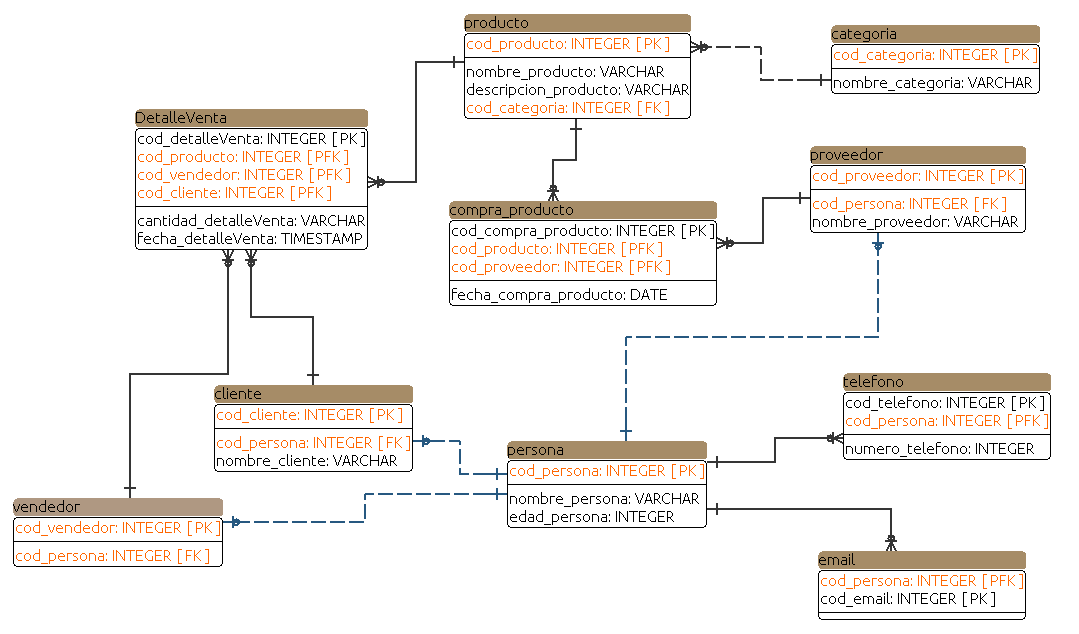
\includegraphics[scale=0.4]{images/modeloER}}
\caption{Modelo ER} 
\floatfoot{\texttt{PFK:} \textit{Primary Foreign Key, llave foranea que a la vez son parte de la llave primaria}\\
\texttt{PK:} \textit{Primary Key, llave primaria}
}
\label{fig:Modelo ER}
\end{figure}
En la Figura \ref{fig:Modelo ER} Modelo ER, podemos observar las distintas entidades de las cuales es necesario identificar las entidades que no hagan referencia aplicando el paso dos del algoritmo podemos identificar una entidad catalogador \emph{categoria} y una entidad que generaliza \emph{persona}, a partir ellas buscamos los que le hacen referencia, \textit{categoria} y \textit{persona} la tomamos como ra\'iz del \'arbol a generar, las entidades que hacen referencia serian \textit{(producto, cliente, vendedor, proveedor, telefono, email)} abajo estar\'ian \textit{(detalleVenta y compra\_producto)} y aplicando el algoritmo se llegar\'ia a la siguiente Figura \ref{fig:ModeloOrdenado} que se encuentra en la p\'agina siguiente.
\begin{figure}[H]
\centering
\subfigure{\includegraphics[scale=0.25]{images/arbol}}
\caption{Modelo Ordenado} \label{fig:ModeloOrdenado}
\end{figure}
\section{Algoritmo de ordenaci\'on \textit{primeros en ser llenado}}
\label{Algoritmo de ordenacion primeros en ser llenado}
Para obtener una lista ordenada de acuerdo al orden que se debe realizar el llenado, se inicia el recorrido de las matrices que trae la matriz bidimensional obtenida del algoritmo anterior, porque si recordamos la lista se orden\'o seg\'un a que una entidad no dependiera de otra entidad, al recorrer podemos encontrarnos que una entidad se repite en distintos lugares, al  inicio de la matriz bidimensional, puede tambi\'en estar listada en medio o al final incluso se puede dar el caso que en uno de las matrices se repita m\'as de una vez. Si vemos la Figura \ref{fig:ModeloOrdenado} la entidad \textit{detalleVenta} se repite m\'as de una vez en la misma fila.

Entonces cual lo tomamos como v\'alido?.
Para lo cual el  recorrido se comienza con el \'ultimo de las matrices que tiene la matriz bidimensional, una vez encontrada las dem\'as que puedan encontrarse en posteriores no llegar\'a a ser v\'alida porque si bien hizo una referencia a un principio ser\'a valida el \'ultimo. Esto se justifica porque si se encuentra al \'ultimo es porque a\'un hace referencia a alg\'un elemento de la matriz anterior al que pertenece, por lo tanto se debi\'o esperar que se llegue hasta ese punto. para el caso de la Figura \ref{fig:ModeloOrdenado} listamos el \'ultimo evitando que se repita.
Para obtener una correcta lista ordenada seg\'un el orden en que deben ser llenados es necesario seguir la siguiente secuencia de pasos:
\begin{enumerate}
\item Crear un matriz de tama\~no de la cantidad de entidades de la base de datos seleccionada.
\item obtener la \'ultima matriz de la matriz bidimensional.
\item Recorrer la matriz y verificar por cada elemento no exista en la matriz del paso uno, en caso de que no exista a\~nadir, en caso de que si no a\~nadir y pasar a la siguiente elemento.
\item Eliminar la \'ultima matriz de la matriz bidimensional.
\item Si existen mas matrices en la matriz bidimensional volver a repetir el paso dos, caso contrario pasar al siguiente paso.
\item Invertir el orden de la matriz del paso uno.
\item Retornar la matriz creado en el paso uno que llegar\'ia a ser el orden que se requiere.
\end{enumerate}
\section{Aplicaci\'on del algoritmo de \textit{primeros en ser llenado}}
Con el algoritmo llegamos a tener el siguiente orden en que debe ser llenado para el ejemplo dado en la figura  \ref{fig:Modelo ER}.
\begin{figure}[H]
\centering
\subfigure{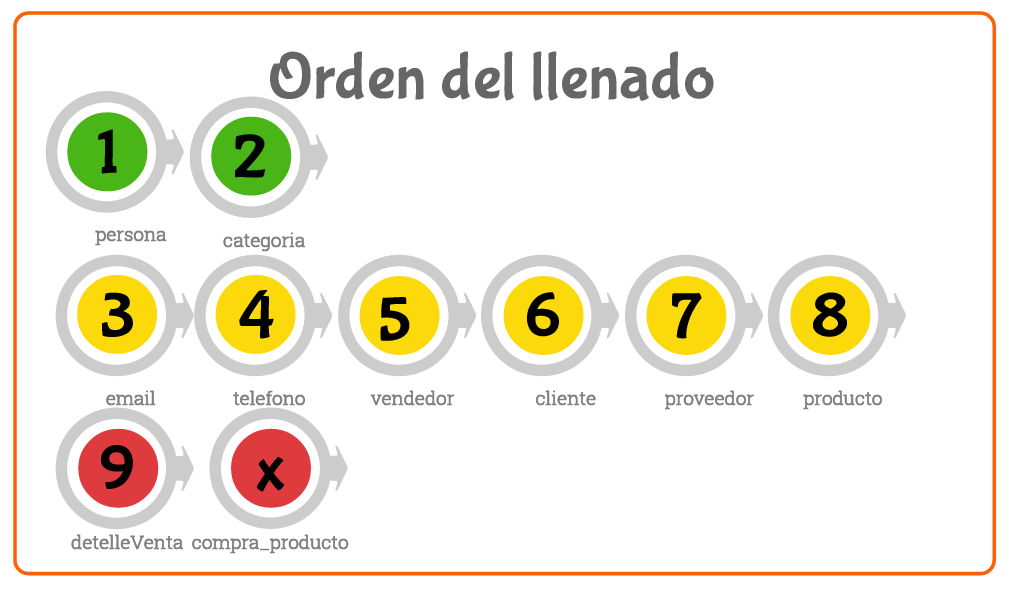
\includegraphics[scale=0.38]{images/ordenCorrecto}}
\caption{Orden de llenado}
\label{fig:Orden de llenado}
\end{figure}
El orden a seguir para este ejemplo es iniciar por el color verde terminando en el color rojo, el orden en cada fila no influye en el resultado permitiendo as\'i la flexibilidad de tomar cualquier elemento para el inicio de cada fila o el conjunto de elementos del mismo color.
\section{Mecanismo de \textit{manejo de referencial} de una base de datos}
Cuando un modelo entidad relaci\'on es llevado a un sistema gestor de base de datos, donde por cada entidad se crea una tabla y las  referencias son representadas mediante las llaves primarias y llaves for\'aneas, En caso de un modelo entidad relaci\'on basado en ER Idioms tiene ciertas caracter\'isticas que son.
\subsection{Llaves primarias compuestas (\texttt{composite keys})}
Cuando se tiene m\'as de un \texttt{primary key}, entre ellas las que son propias de la tabla y otras pertenecientes a las que referencia que vienen como primarias, llegan a formar parte del \texttt{primary key} de la tabla, formando as'i \texttt{composite keys} para la misma. En conceptos de entidad relaci\'on en la figura  \ref{fig:llaves compuestas} se puede observar  las entidades que hacen referencia a otra.
\begin{figure}[H]
\centering
\subfigure{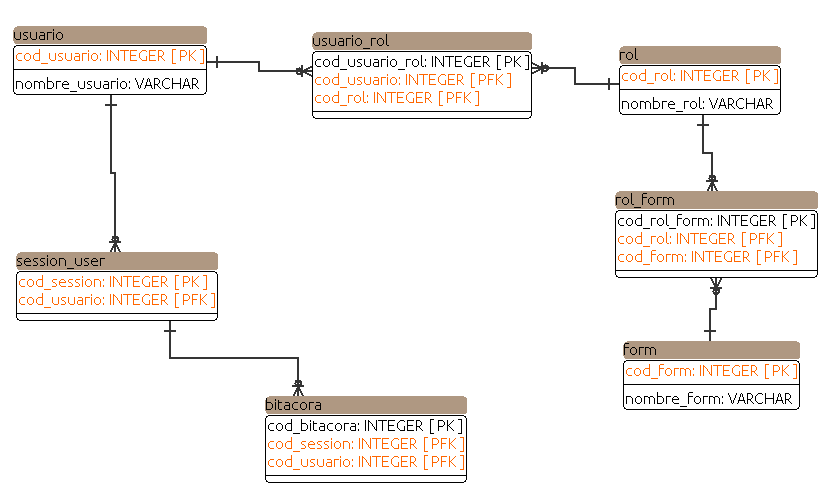
\includegraphics[scale=0.5]{images/llavesCompuestas}}
\floatfoot{\texttt{PFK:} \textit{Primary Foreign Key, llave foranea que a la vez son parte de la llave primaria}\\
\texttt{PK:} \textit{Primary Key, llave primaria}}
\caption{Llaves compuestas} \label{fig:llaves compuestas}
\end{figure}
Donde se puede ver que la entidad \textit{usuario\_rol} hace referencia a las entidades \textit{usuario} y \textit{rol}, las tres entidades llegar\'ian a formar una composici\'on  (\textit{usuario\_rol} compone de \textit{usuario} y \textit{rol}) donde la existencia de \textit{usuario\_rol} es dependiente de las que compone. Si este modelo lo llevamos a un gestor de base de datos un DBMS se llega a tener como en la figura \ref{SQLtablaUsuarioRolComposite}.\\
\lstset{language=sql,breaklines=true}
\label{SQLtablaUsuarioRolComposite}
\captionof{lstlisting}{SQL tabla usuario\_rol}
\begin{lstlisting}
CREATE TABLE usuario_rol(
  cod_usuario_rol serial NOT NULL,
  cod_usuario INTEGER NOT NULL,
  cod_rol INTEGER NOT NULL,
  CONSTRAINT cod_usuario_rol PRIMARY KEY (cod_usuario_rol,cod_usuario,cod_rol),
  CONSTRAINT rol_usuario_rol_fk FOREIGN KEY (cod_rol)
      REFERENCES rol (cod_rol) MATCH SIMPLE
      ON UPDATE NOT ACTION ON DELETE NOT ACTION,
  CONSTRAINT usuario_usuario_rol_fk FOREIGN KEY (cod_usuario)
      REFERENCES usuario (cod_usuario) MATCH SIMPLE
      ON UPDATE NOT ACTION ON DELETE NOT ACTION
)
\end{lstlisting}
El \texttt{primary key} propia es independiente en cambio \textit{cod\_usuario} es perteneciente a la tabla \textit{usuario} pero viene como \texttt{primary key} lo mismo sucede con el campo \textit{cod\_rol}  que pertenece a la tabla \textit{rol}, como ambas \texttt{foreing key} vienen como \texttt{primary key} la tabla \textit{usuario\_rol} llegar'ia a tener un \texttt{primary key} compuesta de tres \textit{cod\_usuario\_rol, cod\_usuario, cod\_rol}. Cuando se quiere hacer una inserci\'on de un registro a la tabla \textit{usuario\_rol} sin antes haber realizado una inserci\'on a las tablas de \textit{usuario} y \textit{rol} cualquier DBMS no lo realiza la inserci\'on por razones de primero debe existir datos en las tablas.
\subsection{Mejor uso de Join}
Al hacer uso de llaves compuestas(\texttt{composite keys}) hace que un identificador llegue m\'as all\'a de lo que normalmente se acostumbra veamos en la figura  \ref{fig:llavesCompuestas}.\\
\begin{figure}[H]
\centering
\subfigure{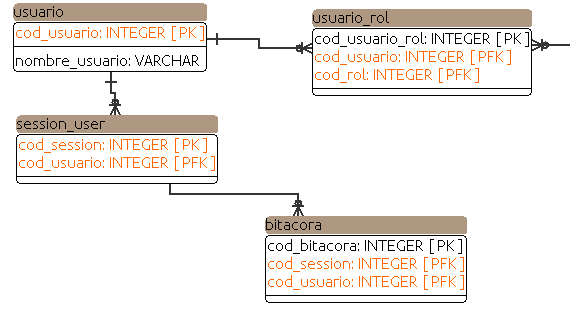
\includegraphics[scale=0.4]{images/join}}
\caption{Modelo E-R con llaves compuestas} \label{fig:llavesCompuestas}
\floatfoot{\texttt{PFK:} \textit{Primary Foreign Key, llave foranea que a la vez son parte de la llave primaria}\\
\texttt{PK:} \textit{Primary Key, llave primaria}}
\end{figure}
Donde en la entidad bit\'acora se tiene tres \texttt{primary key} llegando a ser una llave compuesta(\texttt{composite key}) y una de ellas es \textit{cod\_usuario} que si bien viene de \textit{session\_user} realmente su origen es en \textit{usuario}, por lo tanto podemos hacer un join entre \textit{bitacora} y \textit{usuario} evitando hacerlo con \textit{session\_user} obteniendo asi una consulta mas eficiente.
\section{Mecanismo de referenciaci\'on}
Cuando generamos datos de prueba para una base de datos es importante tener en cuenta el manejo de las llaves compuestas(\texttt{composite keys}), no podemos generar al azar los \texttt{foreign key} porque se llegar'ia a tener problemas de inconsistencia.

Una t\'ecnica para evitar los problemas de inconsistencia es tener como fuente la tabla al que se referencia y los atributos  tomarlo como base para la generaci\'on de \emph{n} datos.
\subsection{Referencia simple}
Las referencias simples son cuando una tabla recibe solo un \texttt{primary key} o \texttt{foreign key} por parte de otra, observemos la figura \ref{SQLUsuarioRolSimple}.
\lstset{language=sql,breaklines=true}
\label{SQLUsuarioRolSimple}
\captionof{lstlisting}{Referencia simple}
\begin{lstlisting}
CREATE TABLE usuario_rol(
  cod_usuario_rol serial NOT NULL,
  cod_usuario INTEGER NOT NULL,
  cod_rol INTEGER NOT NULL,
  CONSTRAINT cod_usuario_rol PRIMARY KEY (cod_usuario_rol,cod_usuario,cod_rol),
  CONSTRAINT rol_usuario_rol_fk FOREIGN KEY (cod_rol)
      REFERENCES rol (cod_rol) MATCH SIMPLE
      ON UPDATE NOT ACTION ON DELETE NOT ACTION,
  CONSTRAINT usuario_usuario_rol_fk FOREIGN KEY (cod_usuario)
      REFERENCES usuario (cod_usuario) MATCH SIMPLE
      ON UPDATE NOT ACTION ON DELETE NOT ACTION
)
\end{lstlisting}
En la figura \ref{SQLUsuarioRolSimple} se puede observar el c\'odigo  \texttt{SQL} (por sus siglas en ingl\'es Structured Query Language) de la tabla \textit{usuario\_rol} de la figura \ref{fig:llaves compuestas}.  La tabla mencionada esta conformada de dos llaves que no son propias de la misma, \textit{cod\_usuario} forma parte de la tabla \textit{usuario} y \textit{cod\_rol} apunta a la tabla \textit{rol}, ambos son campos que apuntan a su respectiva tabla de manera \'unica por lo tanto se deja entender que se hace una referencia simple de llaves.
\subsection{Referencia compuesta}
Las referencias compuestas son cuando una tabla recibe m\'as de un \texttt{primary key} o \texttt{foreign key} por parte de otra. Es importante tomar los atributos que apuntan a otra como un conjunto de atributos para manejar como base para la generaci\'on de los datos requeridos.
\lstset{language=sql,breaklines=true}
\label{lst:SQLReferenciaCompuesta}
\captionof{lstlisting}{Referencia compuesta}
\begin{lstlisting}
CREATE TABLE bitacora(
  cod_bitacora serial NOT NULL,
  cod_session INTEGER NOT NULL,
  cod_usuario INTEGER NOT NULL,	  
  CONSTRAINT bitacora_pk PRIMARY KEY (cod_bitacora,cod_session,cod_usuario),
  CONSTRAINT session_user_bitacora_fk FOREIGN KEY (cod_session,cod_usuario)
      REFERENCES "session_user" (cod_session,cod_usuario) MATCH SIMPLE
      ON UPDATE NOT ACTION ON DELETE NOT ACTION
)
\end{lstlisting}
En la figura \ref{lst:SQLReferenciaCompuesta} el campo \textit{cod\_session} y \textit{cod\_usuario} de la tabla \textit{bitacora} hace referencia a \textit{session\_user} a los campos \textit{cod\_session} y \textit{cod\_usuario}, son dos campos que apuntan a la misma tabla que este caso \textit{session\_user} por lo tanto llegar\'ia a ser una referencia compuesta.
%% Los cap'itulos inician con \chapter{T'itulo}, estos aparecen numerados y
%% se incluyen en el 'indice general.
%%
%% Recuerda que aqu'i ya puedes escribir acentos como: 'a, 'e, 'i, etc.
%% La letra n con tilde es: 'n.

\chapter{Algoritmos de ordenamiento y mecanismos de manejo referencial}
\label{Algoritmos de ordenamiento y mecanismos del manejo referencial}
Una base de datos relacional esta fuertemente ligada al concepto Entidad Relaci\'on \cite{FBD}(E-R ``Entity Relationship"). Una entidad que representa gr\'aficamente a un concepto del mundo real o abstracta, que da lugar a una tabla en la base de datos. Una relaci\'on entre dos o m\'as entidades describe alguna interacci\'on entre las mismas, el tipo de relaci\'on  dar\'a lugar a un comportamiento entre las entidades involucradas \cite{introbasedatos}.

En un modelo Entidad Relaci\'on (E-R) para base de datos basados en ER Idioms\cite{idioms}, se tiene patrones de dise\~no m\'as definidos, las relaciones que llegan a tener entre entidades y la forma en que se hacen da lugar pr\'acticamente a siguientes siete patrones de dise\~no para un modelo ER.
\begin{enumerate}
\item Una entidad que no hace referencia a otra pero si es referenciada es una entidad de tipo \textit{catalogo}. Act\'ua como un tipificador y generalmente almacenan peque\~nas cantidades de datos, los datos que se almacenan  se conocen a priori y la cantidades de datos son predecibles lo cual no significa que sean estables pueden llegar ha incrementarse, la entidad que hace referencia al \textit{catalogo} llega a ser una entidad de tipo \textit{catalogado}.
\item En algunos casos se tiene entidades que se encuentran sueltas por lo tanto no hacen referencia ni son referenciadas por ninguna otra, la cual es una entidad de tipo \textit{simple}.
\item En un modelo entidad relaci\'on donde una entidad hace referencia a m\'as de una y que su existencia depende de las mismas, a todo este conjunto se le denomina  \textit{composici\'on}, consiste en que puede componer de m\'as de dos incluy\'endose as\'i mismo.
\item
Cuando una entidad es dependiente de la existencia de otra al que detalla es de tipo \textit{detalle} de la alguna entidad maestra, donde el  detalle obedece a la maestra, a diferencia de un catalogador en un maestro no se puede determinar  los posibles datos a priori ni mucho menos estimar la cantidad aproximada de datos que pueda tener y que generalmente almacena cantidades grandes de datos.
\item
Hay veces que una entidad referencia a otra del mismo tipo llegando a ser una relaci\'on recursiva la cual llega a ser una entidad de tipo \textit{reflexivo simple}, cuando se implementa este tipo de relaci\'on es importante tener en cuenta que la relaci\'on no debe ser de obligatoriedad.
\item
En ocasiones es necesario relacionar entidades del mismo tipo y guardar una historia de ellas, la forma de representar este concepto es que una entidad representa la forma que se relacionan la entidad que hace una doble referencia, lo cual lleva a ser una entidad tipo  \textit{reflexivo compuesto}.
\item
Cuando se quiere hacer una especializaci\'on a una entidad en particular esta llega a ser la entidad hija de de la entidad generalizada este tipo de relaci\'on es conocida como \textit{is a} en idioms.
\end{enumerate}

\section{T\'ecnicas de ordenamiento}
En una base de datos las tablas tienen una secuencia de prioridades en el llenado de datos, una manera de obtener esta secuencia es buscar todas las tablas que no tengan ningun \texttt{foreign key}, posteriormente las tablas que tienen como \texttt{foreign key} que referencian a las anteriores que llenamos y asi sucesivamente de manera secuencial, hasta acabar con el ultimo al que no referencia ninguna otra tabla, esto llegar a ser confuso sobre todo si son muchas tablas al momento de hacer el llenado, para lo cual es necesario alguna t'ecnica para el orden correcto del llenado.

La propuesta en este proyecto sobre la t\'ecnica para obtener el orden seg\'un la prioridad en que deben ser llenado las tablas, es identificar primero todas aquellas que son un entidad catalogador, simples y  aquellas que no dependen de ninguna otra en las que puede que en algunos casos pueden estar las entidades maestras  o las que son padres de una generalizaci\'on, los  siguientes a identificar son los catalogados, las que hacen referencia a las identificadas anteriormente pero que estas no deben depender de otras que a\'un no se llen\'o para evitar  tener problemas de inconsistencia. 
\section{Algoritmo de ordenamiento}
\label{Algoritmo de ordenamiento}
Para obtener la lista de tablas seg\'un el orden en que debe ser llenado una base de datos,  es necesario aplicar el siguiente algoritmo:
\begin{enumerate}
\item Crear una matriz bidimensional.
\item Seleccionar las entidades de tipo catalogo, simples, maestras que no dependan de otra entidad y entidades que sean de tipo \textit{reflexivo simple} pero que no hagan referencia a otra distinta de el, para luego almacenar este conjunto en una matriz lineal y que est a su ves agregarlo en la matriz bidimensional.
\item De la matriz bidimensional obtener la \'ultima matriz y por cada elemento buscar todas las entidades que le hagan referencia y agregarlos en un nuevo arreglo lineal, una vez recorrido todos los elementos a\~nadir el arreglo lineal en el arreglo bidimensional.
\item Verificar que se ha recorrido todas las entidades, en caso de que se recorri\'o todo pasar al paso cinco, en caso contrario repetir el paso tres.
\item si se llego hasta aqu\'i es porque ya tenemos un arreglo bidimensional ya con el orden pero esta aun no es la lista para lo que requerimos ya que se da el caso que se pueda repetir mas de una ves el nombre de una entidad en los distintos matrices que contiene la matriz bidimensional por lo tanto es necesario aplicar el algoritmo de ordenaci\'on primeros en ser llenados a la matriz bidimensional.
\end{enumerate}
\section{Aplicaci\'on del algoritmo}
\begin{figure}[H]
\centering
\subfigure{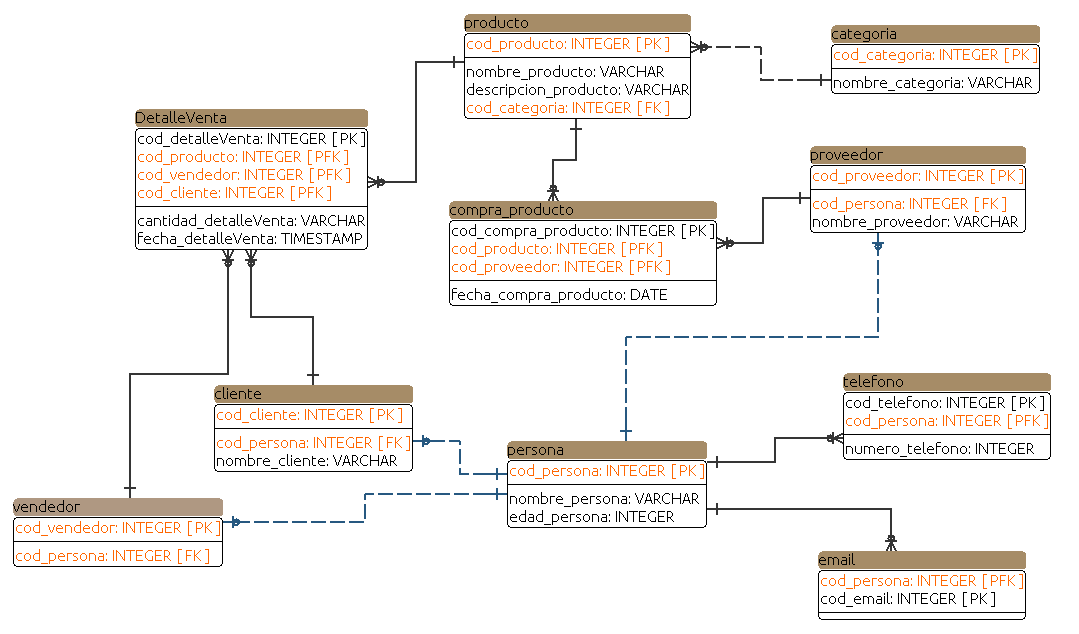
\includegraphics[scale=0.4]{images/modeloER}}
\caption{Modelo ER} 
\floatfoot{\texttt{PFK:} \textit{Primary Foreign Key, llave foranea que a la vez son parte de la llave primaria}\\
\texttt{PK:} \textit{Primary Key, llave primaria}
}
\label{fig:Modelo ER}
\end{figure}
En la Figura \ref{fig:Modelo ER} Modelo ER, podemos observar las distintas entidades de las cuales es necesario identificar las entidades que no hagan referencia aplicando el paso dos del algoritmo podemos identificar una entidad catalogador \emph{categoria} y una entidad que generaliza \emph{persona}, a partir ellas buscamos los que le hacen referencia, \textit{categoria} y \textit{persona} la tomamos como ra\'iz del \'arbol a generar, las entidades que hacen referencia serian \textit{(producto, cliente, vendedor, proveedor, telefono, email)} abajo estar\'ian \textit{(detalleVenta y compra\_producto)} y aplicando el algoritmo se llegar\'ia a la siguiente Figura \ref{fig:ModeloOrdenado} que se encuentra en la p\'agina siguiente.
\begin{figure}[H]
\centering
\subfigure{\includegraphics[scale=0.25]{images/arbol}}
\caption{Modelo Ordenado} \label{fig:ModeloOrdenado}
\end{figure}
\section{Algoritmo de ordenaci\'on \textit{primeros en ser llenado}}
\label{Algoritmo de ordenacion primeros en ser llenado}
Para obtener una lista ordenada de acuerdo al orden que se debe realizar el llenado, se inicia el recorrido de las matrices que trae la matriz bidimensional obtenida del algoritmo anterior, porque si recordamos la lista se orden\'o seg\'un a que una entidad no dependiera de otra entidad, al recorrer podemos encontrarnos que una entidad se repite en distintos lugares, al  inicio de la matriz bidimensional, puede tambi\'en estar listada en medio o al final incluso se puede dar el caso que en uno de las matrices se repita m\'as de una vez. Si vemos la Figura \ref{fig:ModeloOrdenado} la entidad \textit{detalleVenta} se repite m\'as de una vez en la misma fila.

Entonces cual lo tomamos como v\'alido?.
Para lo cual el  recorrido se comienza con el \'ultimo de las matrices que tiene la matriz bidimensional, una vez encontrada las dem\'as que puedan encontrarse en posteriores no llegar\'a a ser v\'alida porque si bien hizo una referencia a un principio ser\'a valida el \'ultimo. Esto se justifica porque si se encuentra al \'ultimo es porque a\'un hace referencia a alg\'un elemento de la matriz anterior al que pertenece, por lo tanto se debi\'o esperar que se llegue hasta ese punto. para el caso de la Figura \ref{fig:ModeloOrdenado} listamos el \'ultimo evitando que se repita.
Para obtener una correcta lista ordenada seg\'un el orden en que deben ser llenados es necesario seguir la siguiente secuencia de pasos:
\begin{enumerate}
\item Crear un matriz de tama\~no de la cantidad de entidades de la base de datos seleccionada.
\item obtener la \'ultima matriz de la matriz bidimensional.
\item Recorrer la matriz y verificar por cada elemento no exista en la matriz del paso uno, en caso de que no exista a\~nadir, en caso de que si no a\~nadir y pasar a la siguiente elemento.
\item Eliminar la \'ultima matriz de la matriz bidimensional.
\item Si existen mas matrices en la matriz bidimensional volver a repetir el paso dos, caso contrario pasar al siguiente paso.
\item Invertir el orden de la matriz del paso uno.
\item Retornar la matriz creado en el paso uno que llegar\'ia a ser el orden que se requiere.
\end{enumerate}
\section{Aplicaci\'on del algoritmo de \textit{primeros en ser llenado}}
Con el algoritmo llegamos a tener el siguiente orden en que debe ser llenado para el ejemplo dado en la figura  \ref{fig:Modelo ER}.
\begin{figure}[H]
\centering
\subfigure{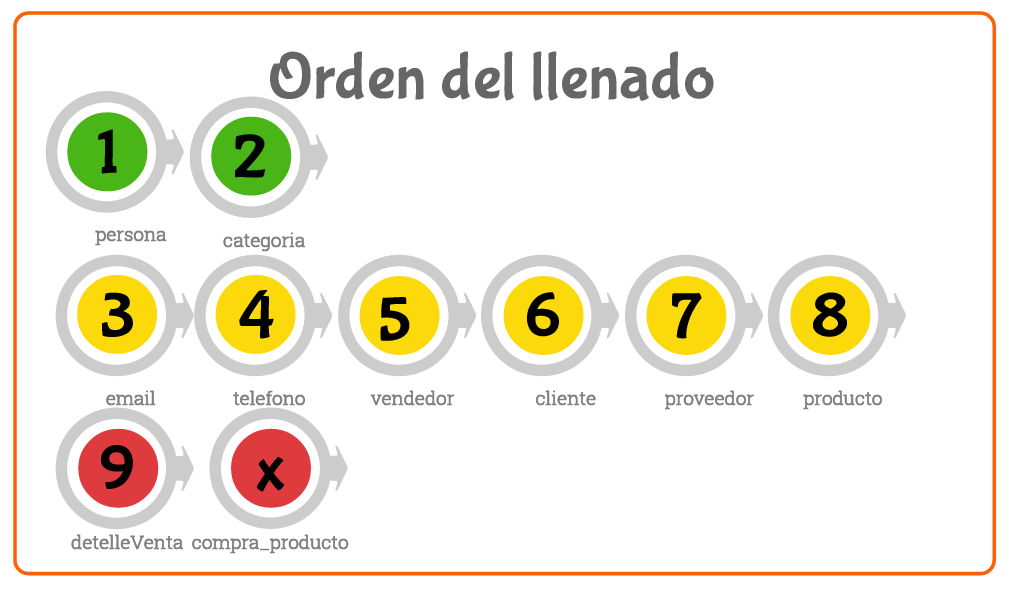
\includegraphics[scale=0.38]{images/ordenCorrecto}}
\caption{Orden de llenado}
\label{fig:Orden de llenado}
\end{figure}
El orden a seguir para este ejemplo es iniciar por el color verde terminando en el color rojo, el orden en cada fila no influye en el resultado permitiendo as\'i la flexibilidad de tomar cualquier elemento para el inicio de cada fila o el conjunto de elementos del mismo color.
\section{Mecanismo de \textit{manejo de referencial} de una base de datos}
Cuando un modelo entidad relaci\'on es llevado a un sistema gestor de base de datos, donde por cada entidad se crea una tabla y las  referencias son representadas mediante las llaves primarias y llaves for\'aneas, En caso de un modelo entidad relaci\'on basado en ER Idioms tiene ciertas caracter\'isticas que son.
\subsection{Llaves primarias compuestas (\texttt{composite keys})}
Cuando se tiene m\'as de un \texttt{primary key}, entre ellas las que son propias de la tabla y otras pertenecientes a las que referencia que vienen como primarias, llegan a formar parte del \texttt{primary key} de la tabla, formando as'i \texttt{composite keys} para la misma. En conceptos de entidad relaci\'on en la figura  \ref{fig:llaves compuestas} se puede observar  las entidades que hacen referencia a otra.
\begin{figure}[H]
\centering
\subfigure{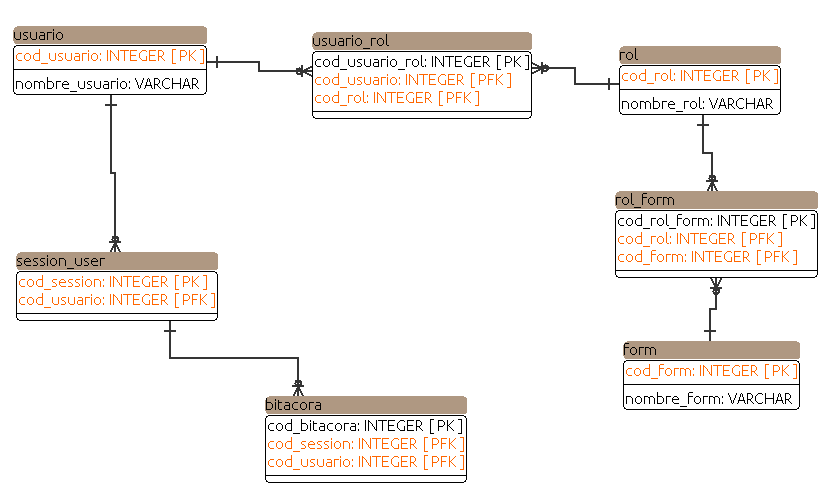
\includegraphics[scale=0.5]{images/llavesCompuestas}}
\floatfoot{\texttt{PFK:} \textit{Primary Foreign Key, llave foranea que a la vez son parte de la llave primaria}\\
\texttt{PK:} \textit{Primary Key, llave primaria}}
\caption{Llaves compuestas} \label{fig:llaves compuestas}
\end{figure}
Donde se puede ver que la entidad \textit{usuario\_rol} hace referencia a las entidades \textit{usuario} y \textit{rol}, las tres entidades llegar\'ian a formar una composici\'on  (\textit{usuario\_rol} compone de \textit{usuario} y \textit{rol}) donde la existencia de \textit{usuario\_rol} es dependiente de las que compone. Si este modelo lo llevamos a un gestor de base de datos un DBMS se llega a tener como en la figura \ref{SQLtablaUsuarioRolComposite}.\\
\lstset{language=sql,breaklines=true}
\label{SQLtablaUsuarioRolComposite}
\captionof{lstlisting}{SQL tabla usuario\_rol}
\begin{lstlisting}
CREATE TABLE usuario_rol(
  cod_usuario_rol serial NOT NULL,
  cod_usuario INTEGER NOT NULL,
  cod_rol INTEGER NOT NULL,
  CONSTRAINT cod_usuario_rol PRIMARY KEY (cod_usuario_rol,cod_usuario,cod_rol),
  CONSTRAINT rol_usuario_rol_fk FOREIGN KEY (cod_rol)
      REFERENCES rol (cod_rol) MATCH SIMPLE
      ON UPDATE NOT ACTION ON DELETE NOT ACTION,
  CONSTRAINT usuario_usuario_rol_fk FOREIGN KEY (cod_usuario)
      REFERENCES usuario (cod_usuario) MATCH SIMPLE
      ON UPDATE NOT ACTION ON DELETE NOT ACTION
)
\end{lstlisting}
El \texttt{primary key} propia es independiente en cambio \textit{cod\_usuario} es perteneciente a la tabla \textit{usuario} pero viene como \texttt{primary key} lo mismo sucede con el campo \textit{cod\_rol}  que pertenece a la tabla \textit{rol}, como ambas \texttt{foreing key} vienen como \texttt{primary key} la tabla \textit{usuario\_rol} llegar'ia a tener un \texttt{primary key} compuesta de tres \textit{cod\_usuario\_rol, cod\_usuario, cod\_rol}. Cuando se quiere hacer una inserci\'on de un registro a la tabla \textit{usuario\_rol} sin antes haber realizado una inserci\'on a las tablas de \textit{usuario} y \textit{rol} cualquier DBMS no lo realiza la inserci\'on por razones de primero debe existir datos en las tablas.
\subsection{Mejor uso de Join}
Al hacer uso de llaves compuestas(\texttt{composite keys}) hace que un identificador llegue m\'as all\'a de lo que normalmente se acostumbra veamos en la figura  \ref{fig:llavesCompuestas}.\\
\begin{figure}[H]
\centering
\subfigure{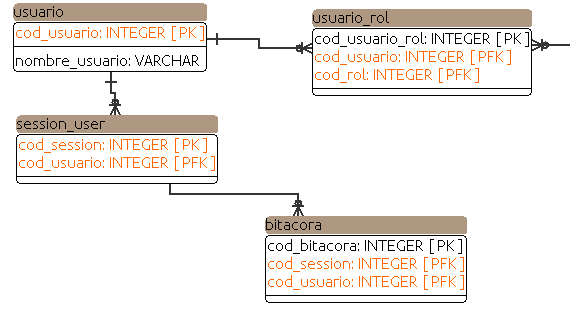
\includegraphics[scale=0.4]{images/join}}
\caption{Modelo E-R con llaves compuestas} \label{fig:llavesCompuestas}
\floatfoot{\texttt{PFK:} \textit{Primary Foreign Key, llave foranea que a la vez son parte de la llave primaria}\\
\texttt{PK:} \textit{Primary Key, llave primaria}}
\end{figure}
Donde en la entidad bit\'acora se tiene tres \texttt{primary key} llegando a ser una llave compuesta(\texttt{composite key}) y una de ellas es \textit{cod\_usuario} que si bien viene de \textit{session\_user} realmente su origen es en \textit{usuario}, por lo tanto podemos hacer un join entre \textit{bitacora} y \textit{usuario} evitando hacerlo con \textit{session\_user} obteniendo asi una consulta mas eficiente.
\section{Mecanismo de referenciaci\'on}
Cuando generamos datos de prueba para una base de datos es importante tener en cuenta el manejo de las llaves compuestas(\texttt{composite keys}), no podemos generar al azar los \texttt{foreign key} porque se llegar'ia a tener problemas de inconsistencia.

Una t\'ecnica para evitar los problemas de inconsistencia es tener como fuente la tabla al que se referencia y los atributos  tomarlo como base para la generaci\'on de \emph{n} datos.
\subsection{Referencia simple}
Las referencias simples son cuando una tabla recibe solo un \texttt{primary key} o \texttt{foreign key} por parte de otra, observemos la figura \ref{SQLUsuarioRolSimple}.
\lstset{language=sql,breaklines=true}
\label{SQLUsuarioRolSimple}
\captionof{lstlisting}{Referencia simple}
\begin{lstlisting}
CREATE TABLE usuario_rol(
  cod_usuario_rol serial NOT NULL,
  cod_usuario INTEGER NOT NULL,
  cod_rol INTEGER NOT NULL,
  CONSTRAINT cod_usuario_rol PRIMARY KEY (cod_usuario_rol,cod_usuario,cod_rol),
  CONSTRAINT rol_usuario_rol_fk FOREIGN KEY (cod_rol)
      REFERENCES rol (cod_rol) MATCH SIMPLE
      ON UPDATE NOT ACTION ON DELETE NOT ACTION,
  CONSTRAINT usuario_usuario_rol_fk FOREIGN KEY (cod_usuario)
      REFERENCES usuario (cod_usuario) MATCH SIMPLE
      ON UPDATE NOT ACTION ON DELETE NOT ACTION
)
\end{lstlisting}
En la figura \ref{SQLUsuarioRolSimple} se puede observar el c\'odigo  \texttt{SQL} (por sus siglas en ingl\'es Structured Query Language) de la tabla \textit{usuario\_rol} de la figura \ref{fig:llaves compuestas}.  La tabla mencionada esta conformada de dos llaves que no son propias de la misma, \textit{cod\_usuario} forma parte de la tabla \textit{usuario} y \textit{cod\_rol} apunta a la tabla \textit{rol}, ambos son campos que apuntan a su respectiva tabla de manera \'unica por lo tanto se deja entender que se hace una referencia simple de llaves.
\subsection{Referencia compuesta}
Las referencias compuestas son cuando una tabla recibe m\'as de un \texttt{primary key} o \texttt{foreign key} por parte de otra. Es importante tomar los atributos que apuntan a otra como un conjunto de atributos para manejar como base para la generaci\'on de los datos requeridos.
\lstset{language=sql,breaklines=true}
\label{lst:SQLReferenciaCompuesta}
\captionof{lstlisting}{Referencia compuesta}
\begin{lstlisting}
CREATE TABLE bitacora(
  cod_bitacora serial NOT NULL,
  cod_session INTEGER NOT NULL,
  cod_usuario INTEGER NOT NULL,	  
  CONSTRAINT bitacora_pk PRIMARY KEY (cod_bitacora,cod_session,cod_usuario),
  CONSTRAINT session_user_bitacora_fk FOREIGN KEY (cod_session,cod_usuario)
      REFERENCES "session_user" (cod_session,cod_usuario) MATCH SIMPLE
      ON UPDATE NOT ACTION ON DELETE NOT ACTION
)
\end{lstlisting}
En la figura \ref{lst:SQLReferenciaCompuesta} el campo \textit{cod\_session} y \textit{cod\_usuario} de la tabla \textit{bitacora} hace referencia a \textit{session\_user} a los campos \textit{cod\_session} y \textit{cod\_usuario}, son dos campos que apuntan a la misma tabla que este caso \textit{session\_user} por lo tanto llegar\'ia a ser una referencia compuesta.
%\include{tecnica}
\chapter{Algoritmos de generaci\'on de datos de prueba}
En el desarrollo de un software que hace uso de una base de datos es muy importante para los desarrolladores sobre todo para los que son encargados de la base de datos, trabajar con una base de datos con datos de prueba  que se asemejen m\'as a las reales tanto en cantidad como en tipo de datos, para eso es necesario tener una cantidad grande de datos de prueba cuanto m\'as mejor, esto nos lleva a un enfoque de generar datos de prueba para base de datos.

Poseer con una cantidad suficiente de datos de prueba no es tan sencillo por lo que un desarrollador normalmente acostumbra hacer la inserci\'on de forma manual lo cual toma un  tiempo excesivo. Cuando se quiere hacer la inserci\'on es necesario tener en cuenta los diferentes tipos de datos que la gran mayor\'ia de los DBMS posee.
\begin{center}
  \scriptsize	
  \captionof{table}{Tipos de datos}
  \label{tablaTipoDatos1} % for use in \ref{table1} if you want to refer to the table number
  \renewcommand{\arrayrulewidth}{1pt}
\begin{tabular}{|p{40mm}|p{98mm}|}\hline
\textbf{Tipo de dato} & \textbf{Caracter\'isticas}\\\hline
\texttt{VARCHAR}(tama\~no) & Almacena cadenas de caracteres de una longitud variable.
La longitud m\'axima son 4000 caracteres \\\hline
\texttt{CHAR}(tama\~no)&
Almacena caracteres con una longitud fija. Siendo 2000 caracteres el máximo\\\hline
\texttt{NUMBER}(precisi\'on, escala) &
Almacena datos num\'ericos, tanto enteros como decimales, con o sin signo. Precisi\'on, indica el n\'umero m\'aximo de d\'igitos que va a tener el dato. Escala, indica el n\'umero de d\'igitos que puede haber a la derecha del punto decimal.\\\hline
\texttt{LONG}&
Almacena cadenas de caracteres de longitud variable. Puede almacenar hasta 2 gigas de informaci\'on\\\hline
\texttt{LONG RAW}&
Almacena datos binarios. Se emplea para el almacenamiento de gr\'aficos, sonidos, etc. Su tamaño m\'aximo es de 2 gigas\\\hline
\texttt{DATE} &
Almacena informaci\'on de fechas y horas.De forma predeterminada almacena un dato con el siguiente formato:siglo/a\~no/mes/dia/hora/minutos/segundos.Este formato se puede cambiar con otros par\'ametros.\\\hline
\texttt{RAW}(tama\~no)&
Almacena datos binarios. Puede almacenar como mucho 2000 bytes.\\\hline
\texttt{ROWID}&
Se trata de un campo que representa una cadena hexadecimal que indica la direcci\'on de una fila en su tabla\\\hline
\texttt{NVARCHAR2}(tama\~no)&
Es similar al varchar2 pero el tama\~no de un car\'acter depende de la elecci\'on del juego de caracteres. El tama\~no m\'aximo es 2000 bytes.\\\hline
\texttt{NCHAR}(tama\~no)&
Similar al \texttt{CHAR} y con las mismas caracter\'isticas que el \texttt{nvarchar2}\\\hline
\texttt{CLOB}&
Similar al \texttt{LONG} y se usa para objectos car\'acter\\\hline
\texttt{BLOB} &
Similar al \texttt{LONG RAW}. Este se usa para objetos binarios.\\\hline
\end{tabular}
\end{center}

Los tipos de datos listadas anteriormente son gen\'ericas en gran parte de lo gestores de base de datos, esta lista no es la misma en lo  gestores de base de datos varia seg\'un el DBMS que incorporan sus tipos de datos personalizadas con caracter\'isticas propias a los tipos de datos de la lista anterior.
\section{Algoritmos de generaci\'on de datos}
La generaci\'on de datos de prueba para base de datos no llega a ser tan sencilla por los diferentes tipos de datos y el l'imite en el tama\~no, pero llega a ser una soluci\'on  para pruebas que se quiera realizar a una base de datos determinada. Para realizar la generaci\'on de datos  es necesario tener algoritmos generadores por cada tipo de datos que tome en cuenta las caracter\'isticas de la misma  y sean capaces de generar cantidades grandes tomando como base una peque\~na cantidad de datos o a lo mejor sin contar ninguna base.
\section{Tipos num\'ericos}
Los tipos num\'ericos consisten en enteros de 2, 4 u 8 bytes y flotantes de 4 u 8, y un n\'umero de presici\'on decimal a elecci\'on.
Los n\'umeros enteros es uno de los m\'as sencillos a generar, con solo incrementar en una unidad al n\'umero  inicial que nos pasan como par\'ametro llegamos en alg\'un momento al l\'imite que tambi\'en se pasa como par\'ametro.
\section{Tipos monetarios}
Los tipos de datos monetarios en realidad se almacenan como un numero cualquiera y que estas tiene similitud con las decimales, el DBMS es quien se encarga de dar el formato necesario. 
\section{Tipos de caracteres}
\subsection{Generaci\'on de nombres}
Para generar nombres es necesario tener una lista o tambi\'en podemos generarlos haciendo combinaciones de las vocales y las consonantes a continuaci\'on haremos una descripci\'on de c\'omo generar aplicando por cada una de ellas.
\subsubsection{Generaci\'on de nombres a partir de vocales y consonantes}
Un nombre esta compuesta generalmente por m\'as de tres caracteres puede que tenga menos y a lo mucho llega a tener 10 a excepci\'on de algunos. Y mucho depende del idioma o el pa\'is.
\begin{figure}[H]
\centering
\subfigure{\includegraphics[scale=0.4]{images/consonantesVocales}}
\caption{Consonantes y vocales} \label{fig:consonantes y vocales}
\end{figure}
Para generar un nombre es importante tener claro lo mencionado anteriormente, para ello aplicamos el siguiente algoritmo para generar nombres haciendo uso de las vocales y consonantes.
\begin{enumerate}
\item Crear una matriz e insertar las cinco vocales.
\item Crear una matriz e insertar las consonantes podemos omitir las que no deseemos usarlas.
\item Generar un n\'umero aleatorio entre 1 a 10 que representa la cantidad de caracteres del nombre y crear una variable al que se le asignar\'a el nombre.
\item Declarar una variable bandera que indicar\'a el turno a quien corresponde sea una vocal o consonante.
\item Preguntamos si la variable bandera indica constante si es verdadero pasamos al siguiente paso 6 caso contrario saltar al paso 7.
\item Generamos un n\'umero aleatorio entre 0 a un m\'aximo de la cantidad de elementos del arreglo de consonantes menos uno, este llega a ser el \'indice del elemento a obtener de las consonantes para luego realizar la concatenaci\'on a la variable que maneja el nombre, contradecir la variable bandera.
\item Generamos un n\'umero aleatorio entre 0 a un m\'aximo de 4 por la cantidad de vocales, esta llega a ser la posici\'on del elemento a obtener del arreglo de vocales y luego concatenamos a la variable que maneja el nombre, contradecir la variable bandera.
\item Preguntamos si el tama\~no del nombre es igual al n\'umero generado en el paso 3, si es verdadero pasamos al paso 9 y si es falso volvemos al paso 5.
\item Finalizamos y retornamos el nombre generado. 
\end{enumerate}
\begin{algorithm}[H]
\begin{algorithmic}[1]
\REQUIRE m\'inimo , m\'aximo de caracteres.\\
\STATE cantidad $\leftarrow$ random(minimo,maximo)
\STATE numero $\leftarrow$ random(0,1)
\STATE cadena $\leftarrow$ $`` "$
\WHILE {$n < cantidad $}
\IF{numero $==$ 0}
\STATE cadena $\leftarrow$ cadena + obtenerVocal
\ELSE
\STATE cadena $\leftarrow$ cadena + ontenerConsonante
\ENDIF
\STATE numero $\leftarrow$ random(0,1)
\ENDWHILE
\RETURN cadena
\end{algorithmic}
\caption{Algoritmo de generaci\'on de palabras}\label{alg:algoritmoGeneracionPalabras}
\end{algorithm}
El Algoritmo~\ref{alg:algoritmoGeneracionPalabras} hace uso de vocales y consonantes para generar palabras.

\subsubsection{Generaci\'on de nombres a partir de una lista de nombres y apellidos}
La generaci\'on de nombre m\'as apellido requiere de una lista de nombre y otro de apellidos, para generar se aplica el siguiente algoritmo:
\begin{figure}[H]
\centering
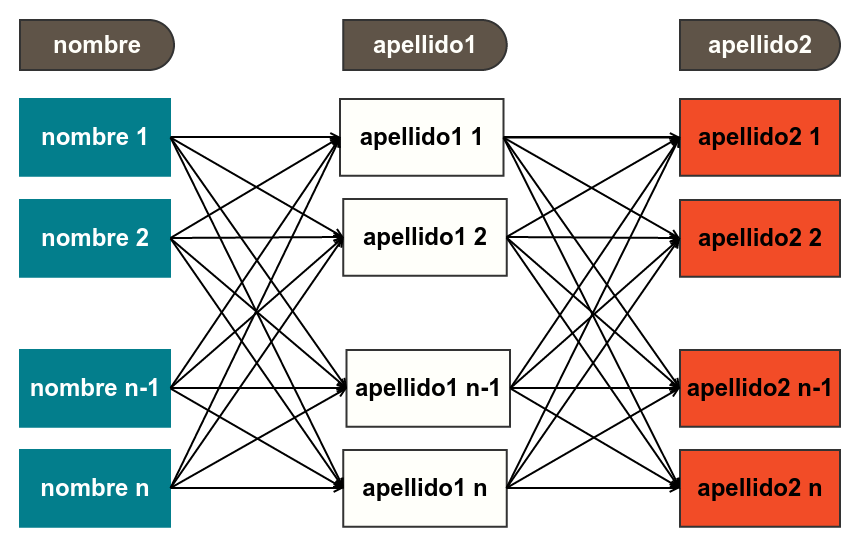
\includegraphics[scale=0.4]{images/listNameApe1Ape2.png}
\caption{Apartir de una lista de nombres}
\end{figure}
\begin{algorithm}[H]
\begin{algorithmic}[1]
\REQUIRE nombres $[$ $]$, apellidosPaternos $[$ $]$,apellidosMaternos $[$ $]$ \label{lin:NombresApellido1Apellido2}
\STATE nombresCombinadas $[$ $]$
\STATE ind
\FOR{iniNomb $\leftarrow$ 0; iniNomb $<$ tamanio(nombres);iniNomb++}
\FOR{iniApePat $\leftarrow$ 0; iniApePat$<$tamanio(apellidosPaternos);iniApePat++}
\FOR{iniApePat $\leftarrow$ 0; iniApePat$<$tamanio(apellidosPaternos);iniApePat++}
\STATE nombresCombinados$[$ind$]$ $\leftarrow$ nombres $[$ iniNomb $]$ + apellidosPaternos $[$ iniApePat $]$ + apellidosMaternos $[$ iniApePat $]$
\ENDFOR
\ENDFOR 
\ENDFOR
\RETURN \TRUE
\end{algorithmic}
\caption{Algoritmo de generacion de nombresLista}\label{alg:algoritmoRaro}
\end{algorithm}
\section{Tipos de datos binarios(Binary Data Types)}

Los sistemas gestores de base de datos(DBMS) permiten almacenar archivos en formatos como \texttt{bytea}, \texttt{blob} entre otros, variando estos segun el DBMS utilizado. 

En este proyecto se pondra a consideracion trabajar con postgresql el cual permite almacenar archivos en formato \texttt{bytea}. El tipo de dato \texttt{bytea} permite almacenar objetos de gran tama\~no, postgreSQL no conoce nada sobre el tipo de informaci\'on que se almacena \texttt{bytea}, simplemente lo considera como una secuencia de bytes.

A momento de generar datos de prueba para base de datos, el tipo de dato \texttt{bytea} llega a ser un caso especial, debido a que no es posible crearlo como cualquier otro dato, como ser un numero de tel'efono que llega a ser combinaciones de n'umeros bajo ciertas condiciones o el caso de un nombre que son combinaciones de vocales y consonantes, sin embargo \texttt{bytea} es posible generar haciendo uso de archivos existentes teniendo solo la ruta del archivo es suficiente para poder insertar en la base datos.
\section{Tipos fecha/hora}
\subsection{Generaci\'on de fechas}
Una fecha esta compuesta por tres partes:
\begin{itemize}
\item A\~no la parte del a\~no para nuestros d\'ias comprende de cuatro d\'igitos desde 1000 hasta el a\~no 9999 el rango no estrictamente establecido.
\item
Mes. la parte del mes se representa en n\'umero de dos d\'igitos que comprende en un rango ya establecida, con un inicio de 01 hasta 12 representando los doce meses del a\~no.
\item
 D\'ia. la cantidad de d\'ias en un mes es variable mucho depende a que mes nos referimos, el rango comprende desde el d\'ia uno y con un final variable desde 28 a 31 d\'ias.
\end{itemize}
Para generar una cantidad de fechas es necesario tener una fecha inicial y final. a partir de ello hacemos la combinaciones para obtener todas las fechas entre el rango dado por par\'ametro veamos en la figura \ref{fig:generacion de fechas}
\begin{figure}[H]
\centering
\subfigure{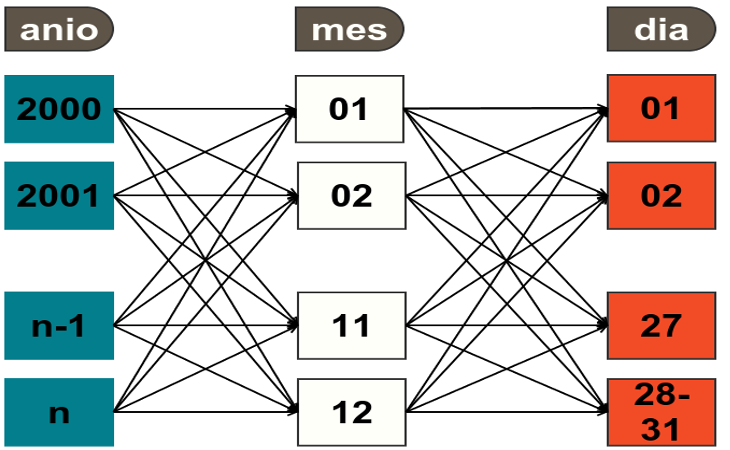
\includegraphics[scale=0.5]{images/algoritmoDates}}
\caption{Generaci'on de fechas} \label{fig:generacion de fechas}
\end{figure}
\subsubsection{Algoritmo de generaci\'on de fechas}
Para realizar la aplicaci\'on del algoritmo de generaci\'on de fechas es necesario tener dos datos una fecha inicial y otra fecha limite final donde es importante que la fecha inicial debe ser una fecha anterior a la final, la cantidad de fechas a obtener depender\'ia del tama\~no de rango que existe entre la inicial y la final.

Veamos el algoritmo de generaci\'on de fechas en formato dd/mm/aa, tomando en cuenta que la cantidad de d\'ias es variable por cada mes adem\'as tomando en cuenta a\~nos bisiestos.
\begin{algorithm}[H]
\begin{algorithmic}[1]
\REQUIRE fechaInicio fechaFinal
\STATE fechas$[$ $]$
\STATE contador $\leftarrow$ 0
\IF{fechaInicio$ < $ fechaFinal}
	\WHILE {fechaInicio $<$ fechaFinal}
	\STATE fechas $[$ contador $]$ $\leftarrow$ fechaInicio+ 1 dia
	\STATE contador $\leftarrow$ contador+1
	\ENDWHILE
\ELSE
	\RETURN error
\ENDIF
\RETURN fechas
\end{algorithmic}
\caption{Algoritmo de generaci\'on de fechas}\label{alg:algoritmoGeneracionFechas}
\end{algorithm}
El algoritmo~\ref{alg:algoritmoGeneracionFechas} es necesario que la fecha inicial sea menor a la fecha final.

\subsection{Generaci\'on de dato tipo Time}
La estructura del dato tipo tiempo es muy similar a las fechas con la diferencia de que estas tienen un rango ya establecidos sin ninguna variaci\'on, esta compuesta por:
\begin{enumerate}
\item Hora. las hora se representa en un n\'umero de dos d\'igitos comenzando desde las 00 horas hasta las 23.
\item Minuto. los minutos tambi\'en se representa en un n\'umero de dos d\'igitos con un inicio en 00 hasta 59 minutos.
\item Segundo. el rango es id\'entica a los de los minutos.
\end{enumerate}
Para generar el tipo de dato time podemos hacer combinaciones de las tres partes que tiene este tipo de dato, realizando combinaciones podemos obtener la cantidad de datos que requerimos.

Veamos la figura siguiente de como hacer las combinaciones:

\begin{figure}[H]
\centering
\subfigure{\includegraphics[scale=0.3]{images/algoritmoTime}}
\caption{Generaci'on de Time} \label{fig:generacion de Time}
\end{figure}
\begin{algorithm}[H]
\begin{algorithmic}[1]
\REQUIRE fechaHoraInicio fechaHoraFinal
\STATE fechasHoras$[$ $]$
\STATE contador $\leftarrow$ 0
\IF{fechaHoraInicio$ < $ fechaHoraFinal}
	\WHILE {fechaHoraInicio $<$ fechaHoraFinal}
	\STATE fechasHoras $[$ contador $]$ $\leftarrow$ fechaHoraInicio+ 1 minuto
	\STATE contador $\leftarrow$ contador+1
	\ENDWHILE
\ELSE
	\RETURN error
\ENDIF
\RETURN fechasHoras
\end{algorithmic}
\caption{Algoritmo de generaci\'on de fecha hora}\label{alg:algoritmoGeneracionDateTime}
\end{algorithm}
El algoritmo~\ref{alg:algoritmoGeneracionDateTime} es necesario que la fecha inicial sea menor a la fecha final.\\
\section{Tipos de direcciones de red}
Las direcciones de red que almacena una base de datos son la IPv4, IPv6 y direcci'on mac.
\subsection{Estructura de una direcci'on IPv4}
Al igual que la direcci'on de una casa tiene dos partes (una calle y un c'odigo postal), una direcci'on IP tambi'en est'a formada por dos partes: el ID de host y el ID de red.
\subsubsection{ID de red}
La primera parte de una direcci'on IP es el ID de red, que identifica el segmento de red en el que est'a ubicado el equipo.
\subsubsection{ID de host}
La segunda parte de una direcci'on IP es el ID de host, que identifica un equipo, un router u otro dispositivo de un segmento.El ID de cada host debe ser exclusivo en el ID de red, al igual que la direcci'on de una casa es exclusiva dentro de la zona del c'odigo postal.

La IPv4 tiene un un formato ( xxx.xxx.xxx.xxx) en que debemos basarnos para generar los limites van establecidos donde (0 $<$ xxx $255$) donde se debe tomar en cuenta que no se usa hasta 255.  
\begin{figure}[H]
\centering
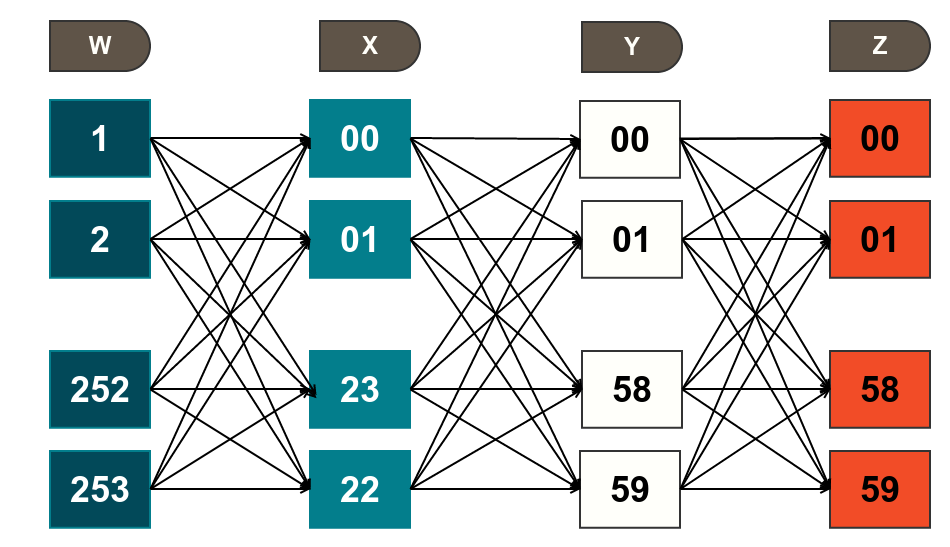
\includegraphics[scale=0.4]{images/ipv4.png}
\caption{Ipv4}
\end{figure}
\begin{algorithm}[H]
\begin{algorithmic}[1]
\REQUIRE inicio final
\STATE direcciones$[$ $]$
\STATE contador $\leftarrow$ 0
\IF{inicio$ < $ fiinal}
	\WHILE {inicio $<$ final}
	\STATE direcciones $[$ contador $]$ $\leftarrow$ inicio+ 1
	\STATE contador $\leftarrow$ contador+1
	\ENDWHILE
\ELSE
	\RETURN error
\ENDIF
\RETURN direcciones
\end{algorithmic}
\caption{Algoritmo de generaci\'on de IPv4}\label{alg:algoritmoGeneracionIPv4}
\end{algorithm}
%\include{mecanismos de almacenamiento}
\chapter{Metadatos}

En este cap'itulo se har'a muestra de las t\'ecnicas necesarias para obtener la estructura de una base de datos, una base de datos existente por lo general lleva tablas que de alguna manera se relacionan entre ellas. El detallar la estructura de una base de datos comprende:
\begin{itemize}
\item Listar todas las tablas de una base de datos.
\item Listar las tablas que hacen referencia y a que tablas.
\item Listar las llaves primarias de una tabla.
\item Listar las llaves for\'aneas de una tabla.
\item Detallar una tablas como ser el tipo de dato, tama\~no, si puede ser nulo etc... 
\end{itemize} 
Es muy importante realizar lo listado anteriormente para obtener la estructura de una base de datos, y usar estos resultados para construir una interfaz gr\'afica de configuraci\'on de generaci\'on de datos de acuerdo a las caracter\'isticas de la columna de una tabla.
Obtener de la estructura de una base de datos puede variar dependiendo del DBMS(Database Managment System) con la que trabajemos, entre los DBMS tenemos a varios entre las mas usadas est\'an MySQL, PostgreSQL, Oracle, SQLServer y otras. En este proyecto se hace la eleccion de  trabajar con postgresSQl las razones para esta elecci\'on son las siguientes.
\begin{itemize}
\item Soporta llaves primarias compuestas(lo cual nos permite aplicar patrones de dise\~no ER Idioms).
\item Es un DBMS de licencia BSD libre.
\end{itemize}
Esto no significa que en las otras no se puedan aplicar este proyecto de lo contrario son aplicables a DBMS relacionales claro que existen diferencias de como manejan los datos internamente cada una de ellas por ejemplo mencionar que postgreSQL los almacena en metadatos todas las tablas que creamos, por lo tanto podemos deducir que para obtener la estructura de una base de datos es necesario trabajar con los metadatos de postgreSQL.
\section{Metadatos en PostgreSQL}
PostgreSQL tiene una arquitectura que involucra muchos estilos, en su nivel mas alto es un esquema cl\'asico cliente-servidor, mientras que el acceso a metadatos es un esquema en capas.
\begin{figure}[H]
\centering
\subfigure{\includegraphics[scale=0.25]{images/arquitecturaPostgres}}
\caption{Arquitectura PostgreSQL \cite{postgresqlpordentro}} \label{fig:ArquitecturaPostgres}
\end{figure}
\begin{itemize}
\item Libpq es el responsable de manipular las comunicaciones entre la aplicaci\'on cliente y el postmaster(Servicio del PostgreSQL en el servidor).
\item El servidor esta compuesto por dos grandes subsistemas, "Postmaster" que es el responsable de aceptar las comunicaciones con el cliente, autentificar y dar acceso. "Postgre" se encarga de la administraci\'on de los consultas(querys) y comandos enviados por el cliente. PostgreSQL trabaja bajo el concepto de "process per user", eso significa un solo proceso cliente por conexi\'on. Tanto el Postmaster como el Postgre deben estar junto en el mismo servidor siempre.
\item El gestor de almacenamiento(Storage Manager) es responsable de la administraci\'on general del almacenamiento de los datos, controla todos los trabajos del back end incluido la administraci\'on del buffer, archivos, bloqueos y control de consistencia de la informaci\'on.   
\end{itemize}
\subsection{Almacenamiento y organizaci\'on de datos}
Los datos siempre se va guardar en ``disco" (esto puede no ser literalmente un Hard Drive).
Esto genera un intenso trabajo de I/O, cuando leemos la data la sacamos de ``disco" para pasarla a la RAM, cuando escribimos la bajamos de la RAM al ``disco".
\begin{figure}[H]
\centering
\subfigure{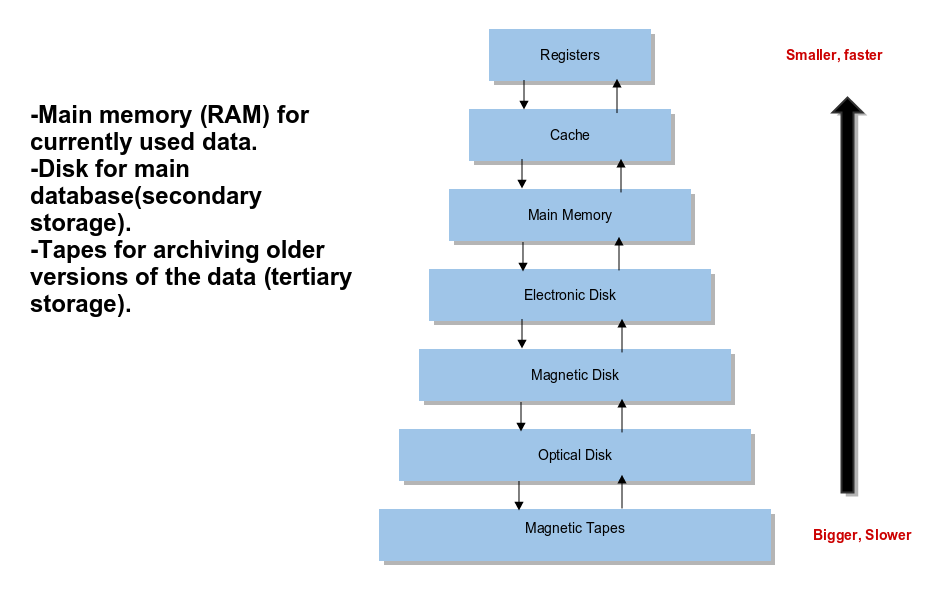
\includegraphics[scale=0.4]{images/almacenamientoorganizaciondatos}}
\caption{Almacenamiento y Organizaci\'on de datos \cite{postgresqlpordentro}} \label{fig:almacenamientoorganizaciondatos}
\end{figure}
PostgreSQL posee un ``Storage Manager" (MySql tiene 5 o m\'as por ejemplo), esta compuesto por varios m\'odulos que proveen administraci\'on de las transacciones y acceso a los objetos de la base de datos.

Los m\'odulos se programaron bajo tres lineamientos bien claros:
\begin{itemize}
\item Manejar transacciones sin necesidad de escribir c\'odigo complejo de recuperaci\'on en caso de ca\'idas.
\item Mantener versiones hist\'oricas  de la data bajo el concepto de ``graba una vez, lee muchas veces".
\item Tomar las ventajas que ofrece el hardware especializado como multiprocesadores, memoria no vol\'atil, etc.  
\end{itemize}
\subsubsection{Los 'indices}
Cada tipo de b\'usqueda tienen un tipo de \'indice adecuado para trabajarla, b\'asicamente un \'indice es un ``archivo" donde est'a parte de un dato y estructura de una tabla con ``search key" de b\'usqueda.\\
\subsection{Como se procesa un consulta(Query)}
\begin{figure}[H]
\centering
\subfigure{\includegraphics[scale=0.25]{images/comoprocesaquery}}
\caption{Como se procesa un query \cite{postgresqlpordentro}} 
\label{fig:comoprocesaquery2}
\end{figure}

Luego pasa por:
 
\lstset{language=sql,breaklines=true}
\begin{lstlisting}
FindExec: found "/var/local/postgres/ ./bin/postgres" using argv[0]
DEBUG: connection: host=[local] user=postgres database=test
DEBUG: InitPostgtres
DEBUG: StartTransactionCommand
DEBUG: query: SELECT firstname
			  FROM friend
			  WHERE age = 33;
			  
[query is proceesd]			  	

DEBUG: ProcessQuey
DEBUG: CommitTransactionCommand
DEBUD: proc_exit(0)
DEBUG: shmen_exit(0)
DEBUG: exit(0)
\end{lstlisting}
 
 \begin{itemize}
 \item Un identificador de reglas de que lo escrito sea sint\'acticamente entendible, que los d\'igitos y los n\'umeros sean reconocibles.
 \item Luego se descompone ``palabra$"$ a ``palabra$"$ el query, para pasar a la estructura que le corresponde seg\'un el query, en este caso a la estructura de un \texttt{SELECT}, esto se ve asi:
\end{itemize}
\lstset{language=sql,breaklines=true}
\label{fig:codigosqlc}
\begin{lstlisting}
simple_select: SELECT opt_distinc target_list
			 into_clause from_clause where_clause
			 group_clause having_clause
			 [
			 	SelectStmt *n = makeNode(SelectStmt);
			 	n->distincClause = $2;
			 	n->targetList = $3;
			 	n->istemp = (bool)((Value *| lfirst($4)))->val.ival;
			 	n->into = (char*) lnext($4);
			 	n->fromClause = $5;
			 	n->whereClause = $6;
				n->groupClause = $7;
				n->havingClause = $8;
				$$ = (Node)n;			 	
			 ]	
\end{lstlisting}

\lstset{language=c,breaklines=true}
\begin{lstlisting}
typedef struct SelectStmt
{
	NodeTag	type;
	List *distincClause;
	
	char *into;
	bool istemp;
	List *targetList;
	List *fromClause;
	Node *whereClause;
	List *groupClause;
	Node *havingClause;
	
	List *sortClause;
	char *portalname;
	bool binary;
	Node *limitOffset;
	Node *limitCount;
	List *forUpdate;
	
	SetOperartion op;
	bool all;
	struct SelectStmt *larg;
	struct SelectStmt *rarg;		
} SelectStmt;	
\end{lstlisting}

\subsubsection{M\'etodos para relacionar tablas}
\subparagraph{Nested loop join}
Consume mas recursos de memoria pero la cantidad de b\'usquedas a realizar a realizar es menor.\\
\subparagraph{Merge join}
Requiere que a data este ordenada para ubicar las relaciones, el costo esta justamente en mantener la data ordenada.
\subparagraph{Hash join}
Aparentemente ser\'ia la forma mas r\'apida de acceder a un dato gracias a la creaci\'on de tablas indexadas, pero limitada a una b\'usqueda de igualdad. Las combinaciones hash requerir'a una combinaci'on de igualdad predicado (un predicado comparaci'on de los valores de una tabla con los valores de la otra tabla utilizando el operador igual $`='$),las combinaciones hash tambi'en puede ser evaluado por un predicado anti-join (un predicado seleccionar valores de una tabla cuando no hay valores relacionados se encuentran en el otro). Dependiendo de los tama\~nos de las tablas, diferentes algoritmos se pueden aplicar.

El ``Executor" toma el plan de ejecuci\'on que el ``planer" le entrega e inicia el procesamiento, ejecuta un ``plan tree".
Este ``plan tree" tiene varios nodos de ejecuci\'on que se van ejecutando uno a uno y de cada uno de ellos se obtiene un set de datos(tuplas). Los nodos tienen subnodos y otros a su vez otros subnodos, tantos como sea necesario.
\section{Obtener la estructura de una base de datos}
En este caso requerimos obtener una estructura de informaci\'on con detalles por cada columna de una tabla semejante a esta:

\texttt{column\_name} $=>$ \texttt{cedula},
 
\texttt{datatype} $=>$ \texttt{integer}, 

\texttt{key} $=>$ \texttt{PRI},

\texttt{is\_nullable} $=>$ \texttt{NO},

\texttt{max\_length} $=>$ \texttt{8}, 

\texttt{column\_default} $=>$

Podemos observar el detalle de un atributo de una tablas por lo tanto podemos hacerlo para cada una y donde:

\texttt{datatype}: es un tipo de dato interno de postgresql.


key: \texttt{UNI} = \texttt{unique}, el campo es un \'indice \'unico.

 
key:	 \texttt{PRI} = \texttt{primary key}, el campo es un \'indice primario, 

key:	 \texttt{FK} = \texttt{foreign key}, el campo es un \'indice de una llave for\'anea.

max\_length: Si el campo es integer, muestra la precisi\'on del entero (2,4,8), si es un varchar, la longitud en caracteres (ej. 75).

column\_default: muestra el tipo de valor por defecto de la tabla; si la tabla es serial, veremos la llamada al nextval de la secuencia: ej. nexval(‘personas\_cliente\_id\_seq'::regclass). Lo que nos permite determinar que campo de nuestra tabla es serial (auto-incremental).

\subsection{Obtener el detalle de una tabla} 
Para entender cada tabla del \textbf{pg\_catalog} debe ser interrogada con el \textbf{oid} de la tabla, que lo sacamos de \textbf{pg\_class}.
Los campos y sus atributos, los sacamos de la tabla \textbf{pg\_attribute}.
El tipo de datos lo sacamos de la tabla \textbf{pg\_type}
los constraints de la tabla los obtenemos de la tabla \textbf{pg\_constraint}
y el valor por defecto, lo sacamos de la tabla \textbf{pg\_attrdef}.
La sentencia construida para sacar esa informaci'on de una sola vez de todas las tablas es esta:
\subsubsection{Usando OIDs}
\lstset{language=sql,breaklines=true}
\label{SQLDetalleTablaMetodo1}
\captionof{lstlisting}{Query para obtener detalle tabla con OIDs}
\begin{lstlisting}
SELECT pgca.attname as column_name,
	      t.typname as data_type,
CASE
		   WHEN cc.contype='p' THEN 'PRI'
		   WHEN cc.contype='u' THEN 'UNI'
		   WHEN cc.contype='f' THEN 'FK'
		   ELSE '' 
END AS key,	
CASE 
		   WHEN pgca.attnotnull=false THEN 'YES' 
ELSE    'NO' 
END AS is_nullable,
CASE 
		   WHEN pgca.attlen=-1 THEN(pgca.atttypmod-4) 
		   ELSE pgca.attlen 
END as max_length,
d.adsrc as column_default
FROM	 pg_catalog.pg_attribute pgca
		   LEFT JOIN pg_catalog.pg_type t ON
			    t.oid=pgca.atttypid
		   LEFT JOIN pg_catalog.pg_class c ON
			    c.oid=pgca.attrelid
		   LEFT JOIN pg_catalog.pg_constraint cc ON 
			    cc.conrelid=c.oid AND 
			    cc.conkey[1]=pgca.attnum
		   LEFT JOIN pg_catalog.pg_attrdef d ON
			    d.adrelid=c.oid AND 
			    pgca.attnum=d.adnum
WHERE c.relname='TABLA' AND
	  pgca.attnum>0 AND
	  t.oid = pgca.atttypid.
\end{lstlisting}
Donde $<$TABLA$>$ representa el nombre de la tabla a la que queremos interrogar para obtener sus metadatos.
Si el modelo de la Figura \ref{fig:Modelo ER} llevamos al gestor de base de datos en este caso PostgreSQL y hacemos uso del c\'odigo de Figura \ref{SQLDetalleTablaMetodo1}  obtendremos algo similar a la siguiente imagen. 
\begin{figure}[H]
\centering
\subfigure{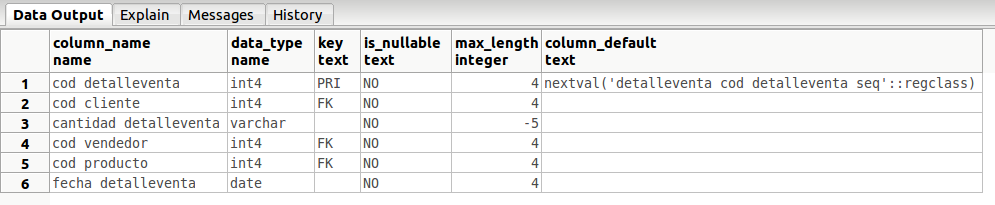
\includegraphics[width=150mm,height=30mm]{images/resDetalleMet1}}
\caption{Detalle tabla OIDs} \label{fig:Detalle Metodo 1}
\end{figure}
Donde:
\begin{itemize}
\item \emph{column\_name} muestra en nombre del columna de la tabla.
\item \emph{data\_type} indica que tipo que almacena esta columna.
\item \emph{key} indica si es una llave sea primaria, for\'anea o sea \'unico.
\item \emph{is\_nullable} nos indica si este campo puede ser nulo.
\item \emph{max\_length} indica el tama\~no de memoria de informaci\'on m\'axima.
\item \emph{colum\_default} en este campo nos indica si es autoincremental en PostgreSQL(serial, bigserial y smallserial) que normalmente se suele usar en llaves primarias las cuales no son obligatorias insertar ya que el DBMS se encarga de realizarlo por nosotros.
\end{itemize}
Son algunos campos almacenadas en el metadato de las muchas que se puede obtener y depende de lo que necesitemos saber, las listadas son b\'asicas sobre la informaci\'on detallada de una determina tabla de una base de datos. El query de la Figura \ref{fig:Detalle Metodo 1} para obtener los metadatos de una tabla no siempre tiene que ser de esa manera podemos hacerlo tambi\'en de la siguientes forma:
\subsubsection{Usando Information schema}
PostgreSQL  a partir de la versi'on 8.0 introdujo el \texttt{INFORMATION\_SCHEMA}. Las vistas definidas en el \texttt{INFORMATION\_SCHEMA} le dan acceso a la informaci'on almacenada en las tablas del sistema PostgreSQL. El \texttt{INFORMATION\_SCHEMA} se define como parte del estandar \texttt{SQL} y encontrar'as un \texttt{INFORMATION\_SCHEMA} en sistemas de bases de datos m'as comerciales (y algunos de c'odigo abierto).Por ejemplo, para ver una lista de las tablas definidas en la base de datos actual, puede ejecutar el comando:
\lstset{language=sql,breaklines=true}
\label{SQLDetalleTablaMetodo2}
\captionof{lstlisting}{Query para detalle obtener el detalle de una tabla information scheme}
\begin{lstlisting}
SELECT tc.column_name,
       data_type,
       character_maximum_length,
       numeric_precision,
       is_nullable,
       tcs.constraint_type,
       column_default,
       check_clause
FROM information_schema.columns AS tc
     LEFT OUTER JOIN
        information_schema.constraint_column_usage AS cc
     	ON tc.table_name = cc.table_name AND
        tc.column_name = cc.column_name
     LEFT OUTER JOIN
        information_schema.table_constraints AS tcs
     	ON tcs.constraint_name = cc.constraint_name
     LEFT OUTER JOIN
        information_schema.check_constraints AS cccs
     	ON cccs.constraint_name = tcs.constraint_name
WHERE tc.table_name = 'NOMBRE DE LA TABLA' AND
      tc.table_schema = 'public' AND
     (tcs.constraint_type='PRIMARY KEY' OR 
      tcs.constraint_type='CHECK' OR 
      tcs.constraint_type ISNULL)
ORDER BY ordinal_position;
\end{lstlisting}
En esta consulta \texttt{SQL} podemos ver las diferencias con la anterior, en esta ya no hacemos uso de los \texttt{OIDS} las tablas que son parte del metadato que usamos son:

\lstset{language=sql,breaklines=true}
\begin{lstlisting}
SELECT * FROM information_schema.columns
SELECT * FROM information_schema.constraint_column_usage
SELECT * FROM information_schema.table_constraints
SELECT * FROM information_schema.check_constraints
\end{lstlisting}
Como resultado tenemos la siguiente informaci\'on:

\begin{figure}[H]
\centering
\subfigure{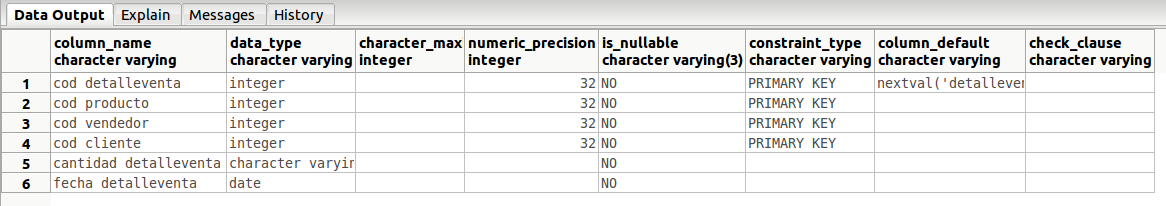
\includegraphics[width=150mm,height=30mm]{images/resDetalleMet2}}
\caption{Information schema} \label{fig:Detalle Metodo 2}
\end{figure}
Donde:
\begin{itemize}
\item \emph{column\_name} muestra en nombre del columna de la tabla.
\item \emph{data\_type} indica el tipo de datos que esta permitido insertar, si comparamos con resultados de la figura \ref{fig:Detalle Metodo 1} aqu\'i nos devuelve el tipo de dato(integer en lugar de int4) como definimos en el modelo de la Figura \ref{fig:Modelo ER} Modelo ER.
\item \emph{constraint\_type} indica si es una llave sea primaria, for\'anea o sea \'unico.
\item \emph{is\_nullable} nos indica si este campo puede ser nulo.
\item \emph{character\_max\_length} indica el tama\~no de memoria de informaci\'on m\'axima.
\item \emph{colum\_default} en este campo nos indica si es autoincrementable en PostgreSQL(serial, bigserial y smallserial) que normalmente se suele usar en llaves primarias las cuales no son obligatorias insertar ya que el DBMS se encarga de realizarlo por nosotros.
\item \emph{check\_clause} en esta columna nos muestra si es campo tiene restricciones sobre la inserci\'on de datos ejemplo: podemos decidir si queremos registrar edades entre 18 a 60 a\~nos. 
\item \emph{numeric precision} nos indica el tama\~no del tipo, aparte de pertenecer a un cierto tipo en los DBMS suelen tener tipos de datos mas precisos.  
\end{itemize}
\subsection{Obteniendo las relaciones entre las tablas}
La estructura de las relaciones entre tablas en una base de datos es el resultado de su modelo ER, donde las relaciones en PostgreSQL son representas por \textit{constraints} en un sistema gestor de base de datos.
\lstset{language=sql,breaklines=false}
\label{SQL Tablas que referencian}
\captionof{lstlisting}{Query para obtener el detalle de referencias}
\begin{lstlisting}
SELECT (SELECT relname
        FROM pg_catalog.pg_class c
        	LEFT JOIN pg_catalog.pg_namespace n ON
		       n.oid = c.relnamespace
        WHERE c.oid=r.conrelid) as tablas,
        conname,
        pg_catalog.pg_get_constraintdef(oid, true) as ref 
FROM pg_catalog.pg_constraint r 
WHERE r.conrelid 
	  IN(SELECT c.oid 
		    FROM pg_catalog.pg_class c LEFT JOIN
           pg_catalog.pg_namespace n ON 
		         n.oid = c.relnamespace 
      WHERE c.relname !~ 'pg_' AND 
            c.relkind = 'r' AND 
            pg_catalog.pg_table_is_visible(c.oid)) AND 
r.contype = 'f'
\end{lstlisting}
De alguna manera necesitamos saber mediante un script las relaciones entre tablas de una base de datos, que tablas se relaci\'on con otra y exactamente que columnas est\'an involucradas, al decir las columnas involucradas nos referimos exactamente a las columnas de una determinada tabla que son las llaves for\'aneas y que estas existen en la tabla que es referenciada, Es lo que precisamente el sript nos da como resultado mostrado en la Figura \ref{fig:Referencias entre tablas}.
\begin{figure}[H]
\centering
\subfigure{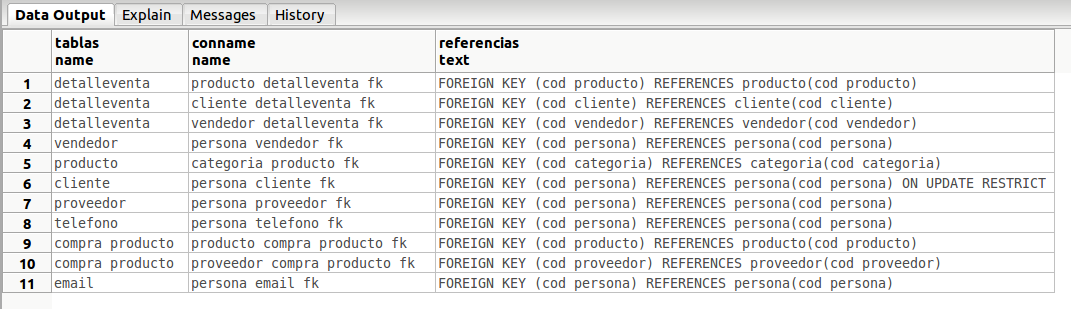
\includegraphics[width=150mm,height=45mm]{images/resReferencias}}
\caption{Referencias entre tablas} \label{fig:Referencias entre tablas}
\end{figure}
En la Figura \ref{fig:Referencias entre tablas} tenemos el resultado de las tablas que llegan a referenciar a otra y las tablas que son referenciadas donde:
\begin{itemize}
\item \textbf{tablas} Nos muestra la lista de tablas que hacen referencia, puede encontrarse que el nombre de una tabla llegue a repetirse en mas de una ocasi\'on no es un problema, detallaremos despu\'es de ver la explicaci\'on de la tercera columna.   
\item \textbf{conname} Muestra el \texttt{CONSTRAINT} de la relaci\'on, que seria algo como en nombre de la relaci\'on entre las tablas involucradas. 
\item \textbf{referencias} En esta columna de la Figura \ref{fig:Referencias entre tablas} nos trae toda la informaci\'on necesaria para ser usado. Analicemos una de ellas.
\lstset{language=sql,breaklines=true}
\begin{lstlisting}
"FOREIGN KEY (cod_producto) REFERENCES producto(cod_producto)"
\end{lstlisting}
La cadena de texto posee informaci\'on relevante donde \emph{(cod\_producto)} es el campo que hace referencia como indica \texttt{REFERENCES} a la tabla \emph{producto} y al campo  \emph{(cod\_producto)}.
Aunque el resultado es en modo texto existen formas de solucionarlo para tener la informaci\'on separada a lo que necesitamos, una manera es realizar un parseo al texto que las distintos lenguajes de programaci\'on ya tienen funciones implementadas para estas tareas. 
\end{itemize}
En la columna \emph{tablas} llegan a repetirse en nombre de una tablas en mas de una vez esto es debido a que nos lista por cada relaci\'on que llegue a tener una tabla con otras
\subsection{Obteniendo las tablas independientes}
Para obtener las tablas que son independientes de otras es necesario usar el script anterior la cual nos entrega un conjunto solo de las tablas que se relacionan de alguna manera entre ellas y tener otro conjunto de todas las tablas de la base de datos, como se tiene estos dos conjuntos de tablas hacemos una operaci\'on de resta entre los conjuntos. La lista de todas las tablas menos la lista de las tablas que se relacionan, como resultado se tiene las tablas que son independientes y que llegar\'ian a ser los primeros en ser llenados.
\lstset{language=sql,breaklines=true}
\label{SQL Tablas independientes}
\captionof{lstlisting}{Query para obtener tablas independientes}
\begin{lstlisting}
SELECT tablename
FROM pg_tables
WHERE schemaname = 'public' AND
      tablename NOT IN
     (SELECT (SELECT relname 
      		      FROM pg_catalog.pg_class c LEFT JOIN
                   pg_catalog.pg_namespace n ON 
                   n.oid = c.relnamespace 
              WHERE
                   c.oid=r.conrelid) as nombre
      FROM pg_catalog.pg_constraint r 
      WHERE r.conrelid IN
            (SELECT c.oid
             FROM pg_catalog.pg_class c LEFT JOIN
                  pg_catalog.pg_namespace n ON 
                  n.oid = c.relnamespace 
             WHERE c.relname !~ 'pg_' AND 
                   c.relkind = 'r' AND 
                   pg_catalog.pg_table_is_visible(c.oid))
      AND r.contype = 'f')
\end{lstlisting}
El c\'odigo SQL para obtener esa informaci\'on es la que vemos en la Figura \ref{SQL Tablas independientes}, si ejecutamos esta consulta nos dar\'ia el siguiente resultado.

\begin{figure}[H]
\centering
\subfigure{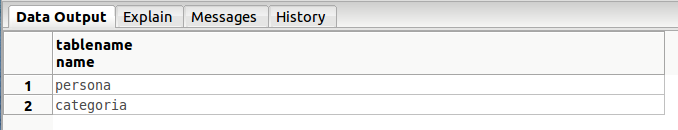
\includegraphics[width=150mm,height=30mm]{images/resTablasInd}}
\caption{Tablas independientes} \label{fig:Tablas independientes}
\end{figure}

Si analizamos la Figura \ref{fig:Modelo ER} Modelo ER del Capitulo \ref{chap:Algoritmos de ordenamiento y mecanismos del manejo referencial} podemos observar que las entidades que son independientes que no hacen referencia a otra son las mismas que nos da como resultado en la Figura \ref{fig:Tablas independientes}.
\section{Ordenando los metadatos}
Si ya contamos con la informaci\'on de los metadatos de una base de datos es necesario por una parte tener claro en el detalle de una tabla, que las llaves for\'aneas pueden ser un conjunto de columnas que hagan referencia a una determinada tabla.

Al momento de hacer las inserciones de datos se debe tener cuidado con este caso si insertamos valores a columnas que hacen referencia estas deben existir en la tabla referenciada veamos un ejemplo:
\begin{figure}[H]
\centering
\subfigure{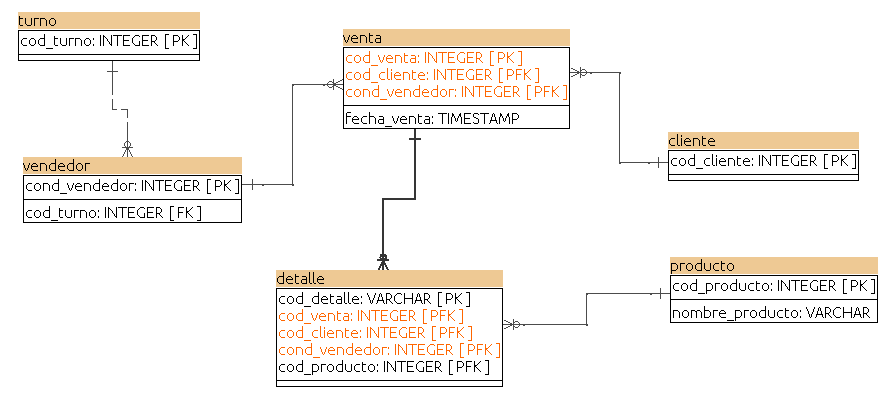
\includegraphics[scale=0.5]{images/ModeloERcomp}}
\caption{Modelo ER compuesto} \label{fig:ModeloERcomp}
\end{figure}
\begin{figure}[H]
\centering
\subfigure{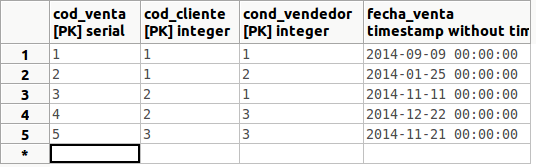
\includegraphics[width=130mm,height=40mm]{images/tablaVenta}}
\caption{Tabla venta} \label{fig:tabla venta}
\end{figure}
\begin{figure}[H]
\centering
\subfigure{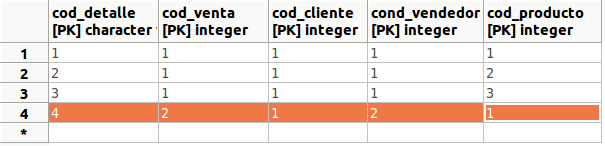
\includegraphics[width=130mm,height=35mm]{images/tablaDetalleCorrecto}}
\caption{Tabla detalle inserci'on correcta} \label{fig:InsercionCorrecta}
\end{figure}

\begin{figure}[H]
\centering
\subfigure{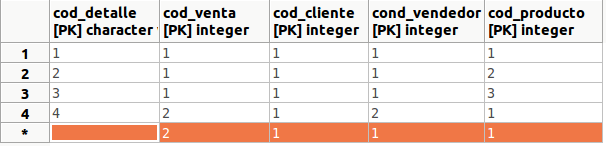
\includegraphics[width=130mm,height=35mm]{images/tablaDetalleIncorrecto}}
\caption{Tabla detalle inserci'on incorrecta} \label{fig:InsercionIncorrecta}
\end{figure}
Como podemos observar en la Figura \ref{fig:ModeloERcomp} la entidad venta es una composici\'on de \textit{vendedor} y \textit{cliente} y que esta a la vez llega ser maestra de la entidad \textit{detalle}, por lo tanto la entidad \textit{detalle} tiene una llave compuesta. Si el modelo lo llevamos a un sistema gestor de base de datos en este caso PostgreSQL y llenamos con uno cuantos datos de prueba como vemos en la Figura \ref{fig:tabla venta} que esta compuesta de llaves compuestas.

Al realizar la inserci\'on en \textit{detalle} debemos tener cuidado en no cometer el error de la ultima inserci\'on que se quiere hacer en la Figura \ref{fig:InsercionIncorrecta}, esta llega a ser incorrecta debido a que no existe una fila de (\textit{cod\_venta,cod\_cliente,cod\_vendedor}) en la tabla \textit{venta} con valores de (\textit{2,1,1}), llegando a no cumplir la integridad referencial adem\'as son datos inconsistentes. La ultima inserci'on de la Figura \ref{fig:InsercionCorrecta} es correcta porque si vemos la tabla Figura \ref{fig:tabla venta} podemos encontrar una fila tambi\'en conocida como tupla que (\textit{cod\_venta,cod\_cliente,cod\_vendedor}) tengan los valores (\textit{2,1,2}) cumpliendo as\'i la integridad referencial y consistencia de datos.
  
  
La otra parte es el ordenar la lista de tablas seg\'un la prioridad que deben ser llenados, esta claro que las tablas independientes son los primeros de ahi en adelante aun no esta claro, por lo tanto es necesario desarrollar mecanismos para obtener una lista de tablas seg\'un el orden en que se requiere.

Para evitar errores de estos dos casos es necesario desarrollar mecanismos que ayuden de alguna manera a solucionar el problema, en el Capitulo \ref{chap:Algoritmos de ordenamiento y mecanismos del manejo referencial}. ya desarrollamos mecanismos de como obtener una lista ordenada haremos aplicaci\'on de dicho algoritmo y como manejar las llaves compuestas para evitar los problemas de la Figura \ref{fig:InsercionIncorrecta}, haremos uso de esas t\'ecnicas.
\subsection{Ordenando las tablas}
La Figura \ref{SQL Tablas independientes} nos da  como resultado las tablas que deben ser llenados primero, las siguientes son algunas de la lista que nos entrega el query de la Figura \ref{SQL Tablas que referencian}, que pr\'acticamente est\'an desordenados.

Si el modelo entidad relaci\'on de la Figura \ref{fig:ModeloERcomp} lo llevamos a postgreSQL y aplicamos el query de la Figura \ref{SQL Tablas que referencian} obtenemos el siguiente resultado:\\
\begin{figure}[H]
\centering
\subfigure{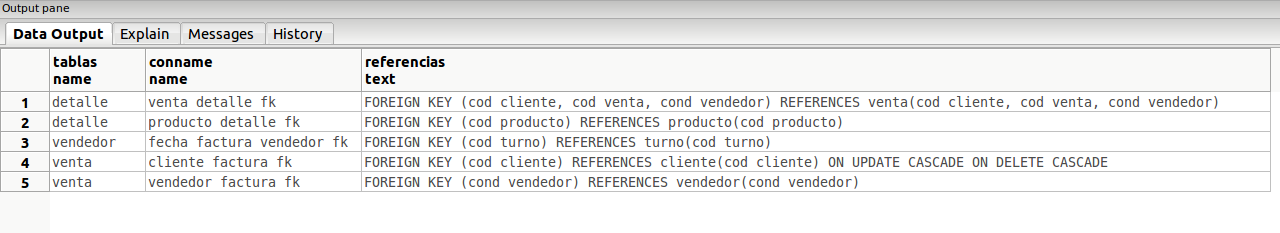
\includegraphics[scale=0.34]{images/referenciasModeloComp}}
\caption{Detalle de relaciones entre tablas} \label{fig:referenciasModeloComp}
\end{figure}
En la Figura \ref{fig:referenciasModeloComp} en la primera columna se tiene en nombre de tablas que hacen referencia a las entidades de la base de datos, pero en la tercera columna no se tiene separada en nombre de la tabla que es referenciada por que es necesario separarlos de alguna manera, analicemos el formato de texto que nos da como resultado para la primera linea perteneciente a \textit{detalle}:
\lstset{language=sql,breaklines=true}
\begin{lstlisting}
"FOREIGN KEY (cod_cliente, cod_venta, cond_vendedor) REFERENCES venta(cod_cliente, cod_venta, cond_vendedor)"
\end{lstlisting}
Lo que haremos es separar en cinco partes la cadena de texto:
\begin{enumerate}
\item \texttt{FOREIGN KEY}
\item \texttt{cod\_cliente, cod\_venta, cond\_vendedor}
\item \texttt{REFERENCES venta}
\item \texttt{cod\_cliente, cod\_venta, cond\_vendedor}
\item ...
\end{enumerate}
Las manera de implementar puede variar de acuerdo a la tecnolog\'ia sea java, php, python etc... sin embargo muchas de estas tecnolog\'ias ya vienen implementadas estas funciones para hacer estas tareas, por ejemplo en java podemos llevar la cadena de texto a un arreglo de textos simplemente definimos delimitadores que este caso serian $`` (  ,  )  "$   obteniendo as\'i un resultado similar a la que listamos. A partir de esa lista escogemos el de la posici\'on 2 iniciando a contar desde 0 que llega ser \textit{REFERENCES venta} en este caso en particular, esta cadena lo volvemos a separar en dos:
\begin{enumerate}
\item \texttt{REFERENCES}
\item \texttt{venta}
\end{enumerate}
Como ya tenemos el nombre de la tabla retornamos este valor como la tabla que es referenciada para \textit{detalle}. Realizamos esto para cada una de la lista de la Figura \ref{fig:referenciasModeloComp}.

Cabe aclarar que en la segunda columna en la segunda separaci\'on de texto que hicimos puede que en algunos casos sobre todo cuando se hace uso de scheme(esquemas) en postgreSQL venga concatenada en nombre del scheme antes del nombre de la tabla concatenada con un punto seguido con el nombre de la tabla ej.

public.venta.

Lo cual no deber\'ia preocuparnos por el simple hecho de que nos ayuda a a identificar en que scheme se encuentra la tabla.Como resultado de las operaciones que se hizo se obtiene el siguiente resultado.
\begin{center}
\scriptsize
  \captionof{table}{tablas que referencian a otra}
  \renewcommand{\arrayrulewidth}{1pt}
  \label{table3} % for use in \ref{table1} if you want to refer to the table number
\begin{tabular}{|p{40mm}|p{98mm}|}
\hline
\textbf{tablas que referencian} & \textbf{tablas referenciadas} \\ \hline
detalle                         & venta                         \\ \hline
detalle                         & producto                      \\ \hline
vendedor                        & turno                         \\ \hline
venta                        & cliente                       \\ \hline
venta                           & vendedor                      \\ \hline
\end{tabular}
\end{center}
En la primera columna se tiene las tablas que hacen referencia y en la segunda columna las que son referenciados. Para hacer uso del algoritmo de ordenaci\'on \ref{Algoritmo de ordenamiento} del Capitulo \ref{Algoritmos de ordenamiento y mecanismos del manejo referencial},  ya contamos con datos hasta el paso dos por lo tanto pasamos al paso tres donde realizamos la b'usqueda para todas aquellas entidades que le hacen referencia a los que son independientes, que para el modelo ER de la Figura \ref{fig:ModeloERcomp} llegar\'ia a ser lo siguiente:
\begin{figure}[H]
\centering
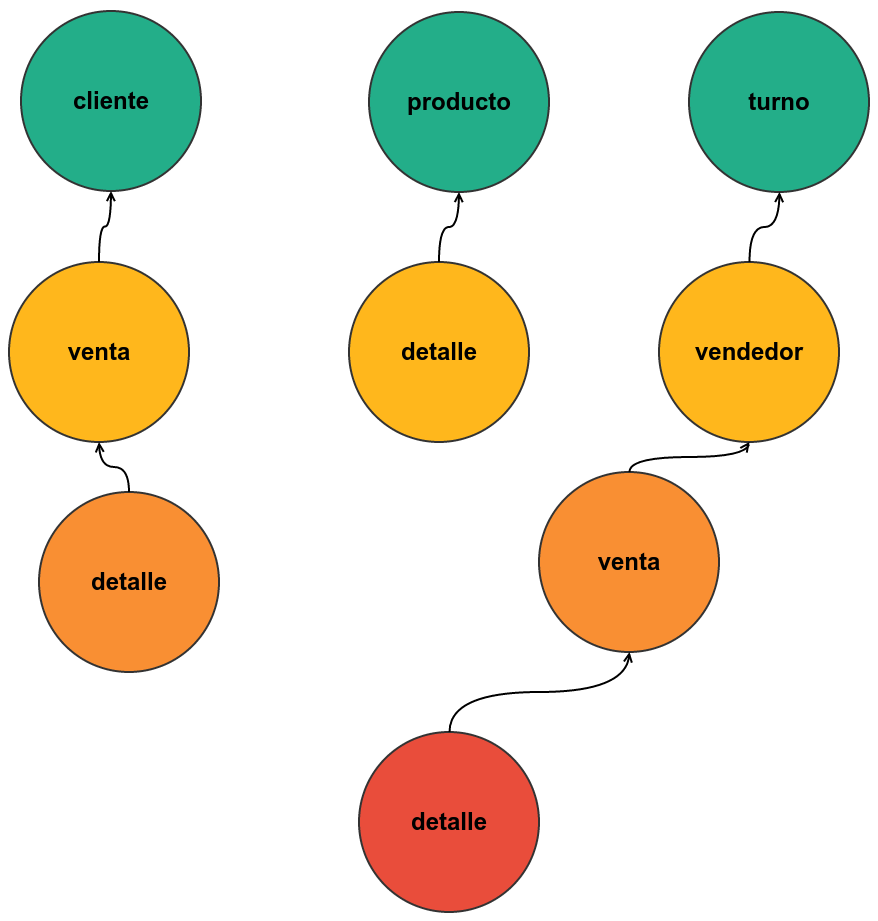
\includegraphics[scale=0.2]{images/desordenadocomp.png}
\caption{Secuencia}
\end{figure}
Donde podemos observar que en nombre de las tablas se llegan a repetir en varios lugares aplicamos el \ref{Algoritmo de ordenacion primeros en ser llenado} de Capitulo \ref{Algoritmos de ordenamiento y mecanismos del manejo referencial} , como resultado llegamos a tener el siguiente orden:
\begin{figure}[H]
 \centering
 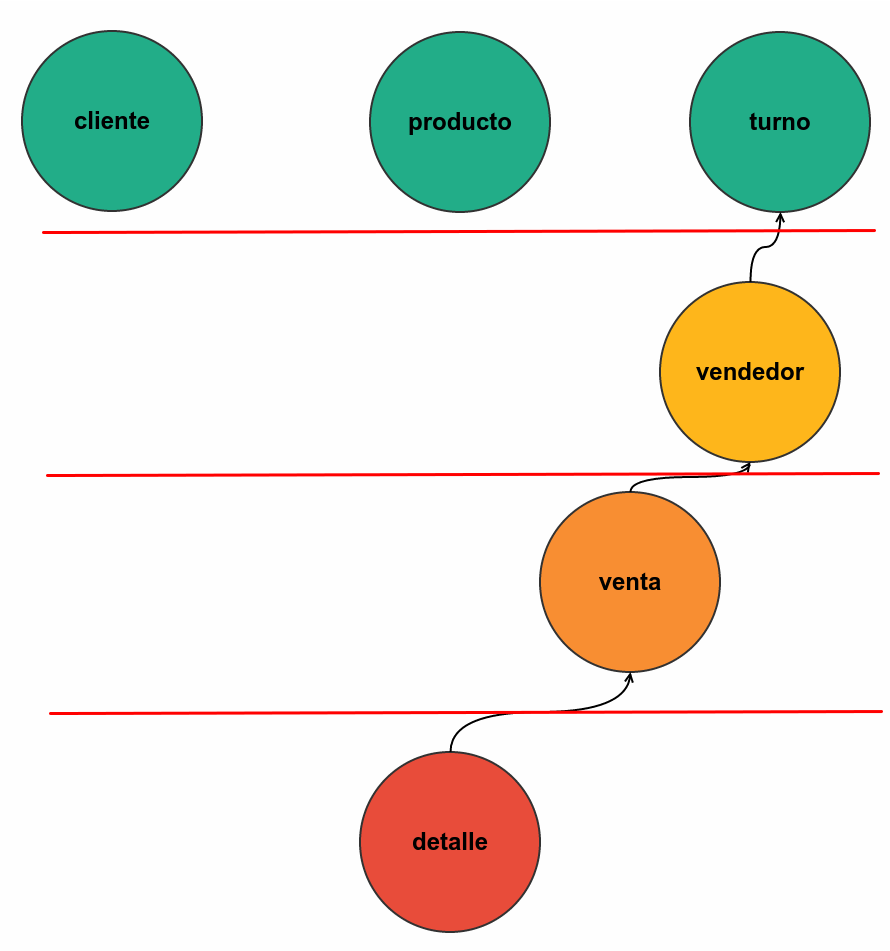
\includegraphics[scale=0.2]{images/ordenadocomp.png}
 \caption{Orden correcto}
 \end{figure}
  
\subsection{Uniendo \texttt{foreign keys}}
Una vez que ya tenemos la informaci\'on detallada por cada una de las tablas que hacen referencia y de las cuales las columnas que est\'en involucradas llegan a ser llaves extranjeras, que si bien pueden ser parte de la llave primaria compuesta de la tabla o simplemente ser una llave for\'anea, al momento de insertar puede llegar a dar lo mismo, por lo tanto no vamos a centrarnos en ese detalle.

La informaci\'on que nos provee el query de la Figura \ref{SQL detalle tabla metodo2} nos da una detallada informaci\'on sobre una tabla en particular pero para lo que necesitamos generar datos de prueba es importante tener mecanismos que eviten cometer errores en las llaves que no son propias de una tabla.Para lo cual haremos uso de \ref{Algoritmo de union de referencias}. En el query de la Figura \ref{fig:referenciasModeloComp} tenemos una informaci\'on valiosa en la tercera columna:

\lstset{language=sql,breaklines=true}
\begin{lstlisting}
"detalle";"venta_detalle_fk";"FOREIGN KEY (cod_cliente, cod_venta, cond_vendedor) REFERENCES venta(cod_cliente, cod_venta, cond_vendedor)"
"detalle";"producto_detalle_fk";"FOREIGN KEY (cod_producto) REFERENCES producto(cod_producto)"
\end{lstlisting}
La tabla \textit{detalle} con las columnas \textit{(cod\_cliente, cod\_venta, cond\_vendedor)} hace referencia a la tabla \textit{venta} a las columnas \textit{(cod\_cliente, cod\_venta, cond\_vendedor)}, adem\'as la columna \textit{(cod\_producto)} hace referencia a la tabla \textit{producto} a la columna \textit{(cod\_producto)}, son las llaves que no son propias de la tabla \textit{detalle}, veamos y analicemos la informaci\'on detallada que nos provee el query de la Figura \ref{SQL detalle tabla metodo2} sobre esta tabla 
 
\begin{figure}[H]
\centering
\subfigure{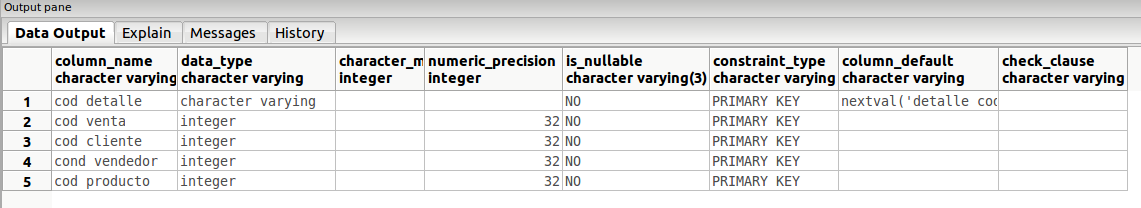
\includegraphics[width=150mm,height=35mm]{images/detalleTablaDetalle}}
\caption{Detalle de la tabla \textit{detalle}} \label{fig:detalleTablaDetalle}
\end{figure}
Fij\'emonos en el detalle que nos da como informaci\'on la Figura \ref{fig:detalleTablaDetalle},  las llaves que no son propias no est\'an agrupadas de acuerdo a la tabla que referenci\'an como sucede en la Figura \ref{fig:referenciasModeloComp} donde si lo agrupa pero solo nos provee esos campos que son llaves que apuntan a otra tabla, a diferencia de la Figura \ref{fig:detalleTablaDetalle} si nos da la informaci\'on de todas las columnas.

El formato detallado de la tabla que necesitamos es unir esas dos informaciones que tenemos obtener algo similar al siguiente cuadro.

\begin{center}
\scriptsize
  \captionof{table}{tabla de referencias para la tabla detalle}
\renewcommand{\arrayrulewidth}{1pt}  
  \label{tableReferenciasTablaDetalle1} % for use in \ref{table1} if you want to refer to the table number
  \begin{tabular}{|l|p{10mm}|p{45mm}|l|l|l|}
\hline
\textbf{\begin{tabular}[c]{@{}l@{}}nombre\\ columna\end{tabular}}                   & \textbf{\begin{tabular}[c]{@{}l@{}}tipo\\ de\\ dato\end{tabular}} & \textbf{es primaria?} & \textbf{serial} & \textbf{\begin{tabular}[c]{@{}l@{}}tabla a\\ la que\\ referencia\end{tabular}} & \textbf{\begin{tabular}[c]{@{}l@{}}columnas a la\\ que referencia\end{tabular}}     \\ \hline
cod\_detalle                                                                        & \texttt{INTEGER}                                                         & \texttt{PRIMARY KEY}  & si              & \texttt{NULL}                                                                         & null                                                                                \\ \hline
cod\_producto                                                                       &                                                                 & FORANEA               &                 & producto                                                                     & cod\_producto                                                                       \\ \hline
\begin{tabular}[c]{@{}l@{}}cod\_venta,\\ cod\_cliente,\\ cod\_vendedor\end{tabular} &                                                                 & FORANEA               &                 & venta                                                                        & \begin{tabular}[c]{@{}l@{}}cod\_venta,\\ cod\_cliente,\\ cod\_vendedor\end{tabular} \\ \hline
\end{tabular}
\end{center}
Si recordamos el query de la figura \ref{SQL Tablas que referencian} da como resultado la lista de tablas que referenci'an en este caso no necesitamos la informaci'on de todos, requerimos espec'ificamente para una tabla determinada. Para lo cual haremos alguna modificaci\'on al query de la Figura \ref{SQL Tablas que referencian} quedando de la siguiente forma:

\lstset{language=sql,breaklines=true}
\label{muestra detalle tabla por tabla}
\captionof{lstlisting}{Query para detalle referencias para una tabla}
\begin{lstlisting}
SELECT(SELECT relname
       FROM pg_catalog.pg_class c 
            LEFT JOIN 
                 pg_catalog.pg_namespace n ON 
                 n.oid=c.relnamespace
       WHERE
            c.oid=r.conrelid) as nombre,
       conname,
       pg_catalog.pg_get_constraintdef(oid,true)AS ref 
FROM
        pg_catalog.pg_constraint r 
WHERE r.conrelid IN
        (SELECT 
                c.oid 
         FROM pg_catalog.pg_class c 
             LEFT JOIN
                pg_catalog.pg_namespace n ON 
                n.oid = c.relnamespace 
         WHERE 
               c.relname !~ 'pg_' AND 
               c.relkind='r' AND 
               pg_catalog.pg_table_is_visible(c.oid))AND
      r.contype = 'f' AND 
        (SELECT relname 
         FROM pg_catalog.pg_class c 
             LEFT JOIN
              pg_catalog.pg_namespace n ON
              n.oid = c.relnamespace 
         WHERE
              c.oid=r.conrelid)='nombreTabla';";
\end{lstlisting}
A diferencia del query de la figura \ref{SQL Tablas que referencian} en este query especificamos exactamente para que tabla queremos saber a quienes referencia agregando al final las siguientes lineas de c\'odigo sql:

\lstset{language=sql,breaklines=true}
\label{muestra detalle tabla por tabla plus}
\captionof{lstlisting}{Parte que determina para una tabla}
\begin{lstlisting}
           AND 
            (SELECT relname 
             FROM pg_catalog.pg_class c 
                  LEFT JOIN
                  pg_catalog.pg_namespace n ON
                  n.oid = c.relnamespace 
             WHERE
                   c.oid=r.conrelid)='nombreTabla';";
\end{lstlisting}
Con la adici'on del c'odigo extra hacemos que no filtre solo para la tabla que requerimos bastara con solo cambiar el \textit{nombreTabla}.
El resultado de este query nos dar\'ia solo los registros donde una determinada tabla hace referencia, veamos para el caso de la tabla \textit{detalle} :

\begin{figure}[H]
\centering
\subfigure{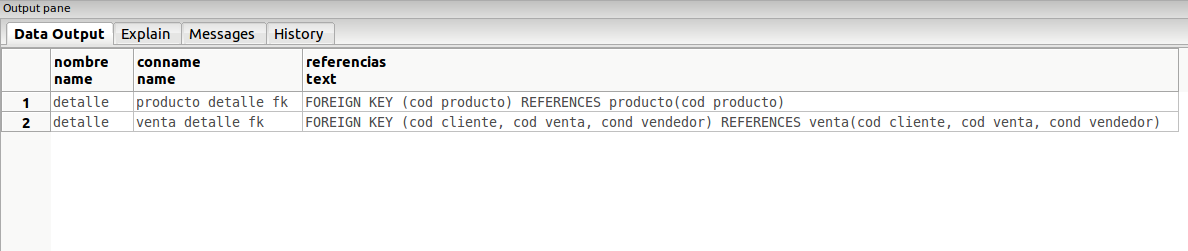
\includegraphics[width=150mm,height=40mm]{images/referenciasTablaDetalle}}
\caption{Detalle de referencias de la tabla detalle} \label{fig:referenciasTablaDetalle}
\end{figure}

Los resultados no llegan a ser tan buenos debido a que nos devuelve en texto todo los datos de las columnas que referenci'an y la tabla que es referenciada con sus respectivos columnas. Haremos uso de las mismas t'ecnicas que aplicamos al momento de realizar el ordenamiento de las tablas seg'un el orden que deben ser llenados que al final necesitamos tener un resultado similar a la siguiente tabla.

\begin{center}
\scriptsize
  \captionof{table}{tabla referencias formateada}
  \label{tablaReferenciasFormateada1} % for use in \ref{table1} if you want to refer to the table number
  \begin{tabular}{|l|l|l|l|}
\hline
\textbf{\begin{tabular}[c]{@{}l@{}}tabla que \\ referencia\end{tabular}} & \textbf{\begin{tabular}[c]{@{}l@{}}columnas que \\ referencian\end{tabular}}           & \textbf{\begin{tabular}[c]{@{}l@{}}tabla \\ referenciada\end{tabular}} & \textbf{\begin{tabular}[c]{@{}l@{}}columnas \\ referenciadas\end{tabular}} \\ \hline
detalle                                                                  & cod\_producto                                                                          & producto                                                               & cod\_producto                                                              \\ \hline
detalle                                                                  & \begin{tabular}[c]{@{}l@{}}cod\_cliente, \\ cod\_venta,\\  cond\_vendedor\end{tabular} & venta                                                                  & cod\_cliente, cod\_venta, cond\_vendedor                                   \\ \hline
\end{tabular}
\end{center}

De la Figura \ref{fig:referenciasTablaDetalle} tomamos la columna 3 y la fila 2 como ejemplo escogemos la fila 2 por razones did'acticas, es donde se encuentra la informaci\'on a en modo texto:
\lstset{language=sql,breaklines=true}
\begin{lstlisting}
"FOREIGN KEY (cod_cliente, cod_venta, cond_vendedor) REFERENCES venta(cod_cliente, cod_venta, cond_vendedor)"
\end{lstlisting}
 La cadena de texto lo separamos en 5 partes:
 
 \textit{Lista en 5 partes}
 \begin{enumerate}
 \item \texttt{FOREIGN KEY}
 \item \texttt{cod\_cliente, cod\_venta, cond\_vendedor}
 \item \texttt{REFERENCES venta}
 \item x\texttt{REFERENCES venta}
 \item ...
 \end{enumerate}
 
 Para obtener esta lista separada llevamos a un arreglo la cadena de texto teniendo como separadores a
 $ ``(" , ``)" $ . La mayor'ia de los lenguajes de programaci\'on ya nos proveen funciones que realicen esta tarea de llevar una cadena de texto a un arreglo con solo indicando los caracteres separadores.
 
 En las la mayor'ia de los lenguajes de programaci'on el conteo de las posiciones se inicia en 0 por tanto vamos basarnos en esa regla, del arreglo solo necesitamos el de la posici'on 1 es donde se encuentra las columnas que hacen referencia en conjunto a la tabla de la posici'on 2 de arreglo sin antes aclarar que este elemento de la posici'on debe ser separado en dos partes:
 
\textit{Lista en 2 partes} 
 \begin{enumerate}
 \item \texttt{REFERENCES}
 \item venta.
\end{enumerate}  

De esta lista solo nos es 'util el de la posici'on 1 es donde encontramos en nombre de la tabla al que se hace referencia.

Si volvemos a la lista que separamos en 5 partes el otro elemento 'util es de la posici'on 3, es donde encontramos las columnas referenciadas.

Realizamos este procedimiento por cada relaci'on que haga la tabla obteniendo as'i un resultado similar a la tabla del cuadro \ref{tablaReferenciasFormateada1}.
Con los resultados obtenidos de la Figura \ref{fig:detalleTablaDetalle} y el de la Figura tabla formateada del cuadro \ref{tablaReferenciasFormateada1} realizamos la union de estos dos resultados para tener una tabla como se ve en el cuadro \ref{tableReferenciasTablaDetalle1}.

Para obtener un resultado del cuadro \ref{tableReferenciasTablaDetalle1} es necesario agregar campos al resultado que nos provee la Figura \ref{fig:detalleTablaDetalle}, agregamos cuatro campos adicionales:
\begin{itemize}
	\item \textit{es\_foranea} En esta columna podemos agregar si es for'anea o no para luego ser evaluado como tal.
	\item \textit{referencian} En esta columna agregamos los nombres de las columnas que hacen referencia a otra tabla.
	\item \textit{tabla} En esta columna agregamos el nombre de la tabla al que referencia.
	\item \textit{referenciados} En esta columna agregamos los nombres de las columnas que son referenciados.
\end{itemize}
Quedando una tabla de la siguiente manera

\begin{center}
\scriptsize
  \captionof{table}{tabla con columnas aumentadas para la tabla \textit{detalle}}
  \label{tablaDetalleAumentadaColumnas1} % for use in \ref{table1} if you want to refer to the table number
  \begin{tabular}{|l|l|l|l|l|l|l|l|}
\hline
column\_name  & data\_type                                                  & constraint\_type & .......... & es\_foranea & \begin{tabular}[c]{@{}l@{}}columnas\\ referencian\end{tabular} & \begin{tabular}[c]{@{}l@{}}tabla\\ referenciada\end{tabular} & \begin{tabular}[c]{@{}l@{}}columnas\\ referenciadas\end{tabular} \\ \hline
cod\_detalle  & \begin{tabular}[c]{@{}l@{}}character\\ varying\end{tabular} & PRIMARY\_KEY     & .........  &             &                                                                &                                                              &                                                                  \\ \hline
cod\_venta    & \texttt{INTEGER}                                                    & \texttt{PRIMARY\_KEY}     &            &             &                                                                &                                                              &                                                                  \\ \hline
cod\_cliente  & \texttt{INTEGER}                                                     & \texttt{PRIMARY\_KEY}    &            &             &                                                                &                                                              &                                                                  \\ \hline
cod\_vendedor & \texttt{INTEGER}                                                     & \texttt{PRIMARY\_KEY}     &            &             &                                                                &                                                              &                                                                  \\ \hline
cod\_producto & \texttt{INTEGER}                                                     & \texttt{PRIMARY\_KEY}     &            &             &                                                                &                                                              &                                                                  \\ \hline
\end{tabular}
\end{center}

Si rocordamos la cadena de texto 
\lstset{language=sql,breaklines=true}
\begin{lstlisting}
"FOREIGN KEY (cod_cliente, cod_venta, cond_vendedor) REFERENCES venta(cod_cliente, cod_venta, cond_vendedor)
FOREIGN KEY (cod_producto) REFERENCES producto(cod_producto)"
\end{lstlisting}
que lo llevamos en un arreglo de 5 elementos, el elemento de la posici'on 1 que llega a ser
\lstset{language=sql,breaklines=true}
\begin{lstlisting}
"cod_cliente, cod_venta, cond_vendedor"
\end{lstlisting}
Es donde encontramos las columnas que hacen referencia por lo tanto a esta cadena necesitamos tambi'en llevarlo a un arreglo lineal donde el car'acter separador llega a ser el $`` , " $  quedando como resultado.
\begin{center}
\scriptsize
\renewcommand{\arrayrulewidth}{1pt}
  \captionof{table}{columnas de la tabla detalle que referencian a venta}
  \label{columnasQueRefencian1} % for use in \ref{table1} if you want to refer to the table number
  \begin{tabular}{|l|l|l|l|}
\hline
\textbf{nombre columna} & cod\_cliente & cod\_venta & cond\_vendedor \\ \hline
\textbf{posicion}       & 0            & 1          & 2              \\ \hline
\end{tabular}
\end{center}


\begin{center}
\scriptsize
\renewcommand{\arrayrulewidth}{1pt}
  \captionof{table}{columna de la tabla detalle que referencia a producto}
  \label{columnaQueRefencian2} % for use in \ref{table1} if you want to refer to the table number
  \begin{tabular}{|l|l|}
\hline
\textbf{nombre columna} & cod\_producto \\ \hline
\textbf{posici'on}      & 0             \\ \hline
\end{tabular}
\end{center}

Los datos del cuadro \ref{columnasQueRefencian1} y \ref{columnaQueRefencian2} son las que hacen referencia a otra tabla para unir las llaves for'aneas y llegar a un resultado como en el cuadro \ref{tableReferenciasTablaDetalle1} para lo cual realizaremos el siguiente procedimiento.

\begin{enumerate}
\item Realizar la uni'on en un arreglo 'unico los elementos del cuadro \ref{columnasQueRefencian1} y \ref{columnaQueRefencian2} llamemosle \textit{referencian} y nos declaramos dos variables denominemosle \textit{pos} y \textit{posTabla} declarada con valor inicial de 0 para controlar la posici'on del nuevo arreglo creado.
\item Obtener el elemento de la la posici'on \textit{pos} y comparar con el elemento de la posici'on \textit{posTabla} del cuadro de \ref{tablaDetalleAumentadaColumnas1} y comparamos si son iguales.
\item Si llegan a ser iguales es porque este campo del cuadro \ref{tablaDetalleAumentadaColumnas1} es un campo que hace referencia a otra entidad por lo tanto agregamos el valor de \textit{true} en su columna \textit{es\_foranea} e incrementar el valor de pos en una unidad y volver al paso 2 asignar un valor de 0 a la variable \textit{posTabla}, de lo contrario pasar al siguiente paso.
\item Es caso de que no sean iguales esta claro que este atributo no hace referencia a ninguna otra tabla y lo agregamos con un valor de \textit{false} y volvemos al paso 2 e incrementar el valor de la variable \textit{posTabla}.
\end{enumerate}
Llegado a un resultado como en el siguiente cuadro:

ESTE CUADRO FALTA REEMPLAZAR POR UNO QUE SERIA COMO QUEDAR'IA
 
\begin{center}
  \captionof{table}{tabla de muestra de atributos for'aneas}
  \label{columnasSeteadasEsForanea1} % for use in \ref{table1} if you want to refer to the table number
  \begin{tabular}{|l|l|}
  \hline 
  \textbf{nombre columna} & cod\_producto \\ \hline
  \textbf{posici'on}      & 0             \\ \hline
  \end{tabular}
\end{center}

En el cuadro \ref{columnasSeteadasEsForanea1} ya se tiene claro que atributos que no son propias y que dependen de la existencia de registros en la tabla a la que referencia, as'i como esta no es como queremos el siguiente procedimiento a realizar es eliminar estos atributos y reemplazarlos por los que tenemos en el cuadro \ref{tablaReferenciasFormateada1}, para realizar este reemplazo necesitamos tener una tabla con los mismo atributos \textit{(tabla\_name , data\_type, check\_clause ... ,referencian,tabla,referenciados)}. Eliminando los atribustos que tengan el valor de \textit{true} en la columna \textit{es\_foranea} llegamos a tener como resultado como el siguiente cuadro

ESTE CUADRO FALTA REEMPLAZAR POR UNO QUE SERIA COMO REALMENTE SE QUIERE

\begin{center}
  \captionof{table}{tabla sin los atributos for'aneas}
  \label{columnasForaneasEliminadas1} % for use in \ref{table1} if you want to refer to the table number
  \begin{tabular}{|l|l|}
  \hline 
  \textbf{nombre columna} & cod\_producto \\ \hline
  \textbf{posici'on}      & 0             \\ \hline
  \end{tabular}
\end{center}
Para obtener la otra tabla con solo de llaves for'aneas aumentamos los campos que llevan a ser similar a la tabla del cuadro \ref{columnasForaneasEliminadas1} realizamos las siguientes operaciones:
 \begin{enumerate}
 \item Crear un arreglo llamemosle \textit{clon} con las mismas dimensiones que del cuadro \ref{tablaDetalleAumentadaColumnas1} y declaramos una variable llamemosle \textit{indice} que hara el control de la pocisi\'on  
 \item Obtenemos la fila de la posici\'on \textit{indice} del cuadro \ref{columnasSeteadasEsForanea1} y verificamos el valor de la columna \textit{es\_foranea} en caso que sea \textit{true} pasamos a 3 y si no hacemos un salto al 4.
 \item A esta fila no lo hacemos la copia en \textit{clon} porque este atributo no es propia de la tabla e incrementamos en una unidad a \textit{'indice}.
 \item Realizamos la copia en \textit{clon} e incrementamos en una unidad a \textit{indice}.
 \item Si no hay mas elementos que comparar pasamos al siguiente de lo contrario volvemos a 2.
 \item Al realizar los pasos anteriores el resultado obtenido ser\'a todas los atributos que son propias de la tabla, al lo cual debemos completar con las restantes que son dependientes de otras tablas pero en una forma diferente,para lo cual tomamos el de la posici'on 1 2 y 3 del arreglo separado en 5 partes que como resultado final se tiene en el cuadro \ref{columnasForaneasEliminadas1}.
 \end{enumerate}
%\chapter{Crear proyecto de configuraci'on}

Cuando se realiza el llenado de datos de prueba sobre una base de datos, hay un inicio y un final donde no siempre se inicia y acaba sin alguna interrupci'on, por muchas razones fallas el'ectricas, cansancio entre otras, para lo cual es importante que toda la informaci'on obtenida en el capitulo anterior sea persistente y que sea posible tener esa informaci'on sin volver a ejecutar los algoritmos adem'as sin la necesidad de volver a conectar a la base de datos.
Para lo cual se almacena en archivos de texto plano con alg'un formato, entre los formatos mas conocidos se tiene a XML (Extensible Markup Language o Lenguaje de Marcas Extensible) y JSON (JavaScript Object Notation - Notaci\'on de Objetos de JavaScript).

\section{JSON (JavaScript Object Notation - Notaci\'on de Objetos de JavaScript)}
Es un formato ligero de intercambio de datos. Leerlo y escribirlo es simple para humanos, mientras que para las m\'aquinas es simple interpretarlo y generarlo. Est\'a basado en un subconjunto del Lenguaje de Programaci\'on JavaScript, Standard ECMA-262 3rd Edition - Diciembre 1999. JSON es un formato de texto que es completamente independiente del lenguaje pero utiliza convenciones que son ampliamente conocidos por los programadores de la familia de lenguajes C, incluyendo C, C++, C\#, Java, JavaScript, Perl, Python, y muchos otros. Estas propiedades hacen que JSON sea un lenguaje ideal para el intercambio de datos.
JSON está constituido por dos estructuras:

\begin{itemize}
\item Una colecci\'on de pares de nombre/valor. En varios lenguajes esto es conocido como un objeto, registro, estructura, diccionario, tabla hash, lista de claves o un arreglo asociativo.
\item Una lista ordenada de valores. En la mayor\'ia de los lenguajes, esto se implementa como arreglos, vectores, listas o secuencias.
\end{itemize}

Estas son estructuras universales; virtualmente todos los lenguajes de programaci\'on las soportan de una forma u otra. Es razonable que un formato de intercambio de datos que es independiente del lenguaje de programaci\'on se base en estas estructuras.

En JSON, se presentan de estas formas:


Un objeto es un conjunto desordenado de pares nombre/valor como se ve en la Figura \ref{fig:objectJSON}. Un objeto comienza con { (llave de apertura) y termine con } (llave de cierre). Cada nombre es seguido por : (dos puntos) y los pares nombre/valor están separados por (coma).
\begin{figure}[H]
\centering
\subfigure{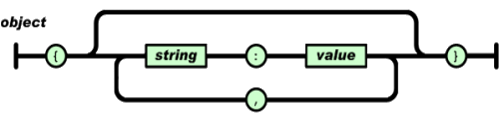
\includegraphics[width=120mm,height=25mm]{images/objectJSON}}
\caption{Object JSON} \label{fig:objectJSON}
\end{figure}

Un arreglo es una colecci\'on de valores. Un arreglo comienza con [ (corchete izquierdo) y termina con ] (corchete derecho) como se ve en la Figura \ref{fig:arrayJSON}. Los valores se separan por , (coma).

\begin{figure}[H]
\centering
\subfigure{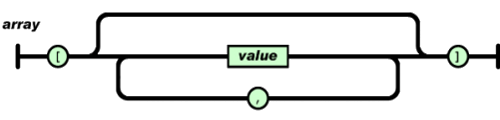
\includegraphics[width=120mm,height=25mm]{images/arrayJSON}}
\caption{Array JSON} \label{fig:arrayJSON}
\end{figure}

Un valor puede ser una cadena de caracteres con comillas dobles, o un n\'umero, o true o false o null, o un objeto o un arreglo como se observa en la Figura \ref{fig:valueJSON}. Estas estructuras pueden anidar

\begin{figure}[H]
\centering
\subfigure{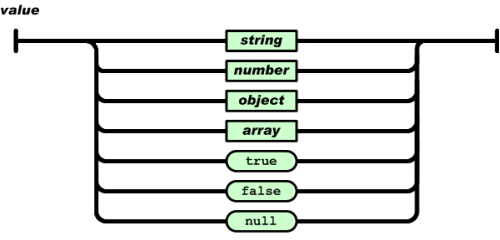
\includegraphics[width=120mm,height=65mm]{images/valueJSON}}
\caption{Value JSON} \label{fig:valueJSON}
\end{figure}

Una cadena de caracteres es una colecci\'on de cero o m\'as caracteres Unicode, encerrados entre comillas dobles, usando barras divisorias invertidas como escape. Un car\'acter est\'a representado por una cadena de caracteres de un \'unico car\'acter ver Figura \ref{fig:stringJSON}. Una cadena de caracteres es parecida a una cadena de caracteres C o Java.

\begin{figure}[H]
\centering
\subfigure{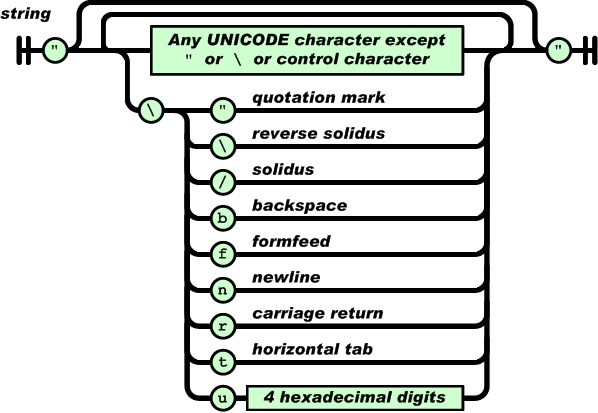
\includegraphics[width=120mm,height=60mm]{images/stringJSON}}
\caption{String JSON} \label{fig:stringJSON}
\end{figure}

Un n\'umero es similar a un n\'umero C o Java, excepto que no se usan los formatos octales y hexadecimales ver la Figura \ref{fig:numberJSON}.

\begin{figure}[H]
\centering
\subfigure{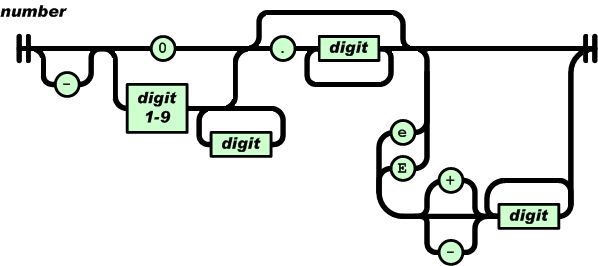
\includegraphics[width=120mm,height=50mm]{images/numberJSON}}
\caption{Number JSON} \label{fig:numberJSON}
\end{figure}

Los espacios en blanco pueden insertarse entre cualquier par de s\'imbolos.

\section{Persistencia de la informaci\'on de metadatos}
La informaci\'on obtenida en el anterior capitulo es necesario que sean persistentes para la reanudaci\'on  en el proceso de configuraci\'on para el objetivo, la informaci'on necesaria a persistir son las siguientes:
\begin{itemize}
\item Datos de la conexi\'on a la base de datos como ser el nombre de la base de datos, usuario, contrase\~na, puerto y el host.
\item La lista de las tablas de la base de datos elegida seg'un al orden en que estos deben ser llenados que se obtuvo en el capitulo anterior.
\item El detalle por cada una de las tablas (nombre de la columna, el tipo de dato, si acepta que sea nulo, si es una llave etc...).  
\end{itemize}
Una alternativa para dar soluci\'on a este requisito es almacenar toda esta informaci'on en archivos sea en el formato JSON o XML, en este proyecto se optar\'a por Json las razones son las siguientes:

\begin{itemize}
\item Soporta dos tipos de estructuras, una de ellas son objetos que contienen una colecci\'on de pares llave-valor y el otro tipo se trata de arrays de valores. Esto proporciona una gran sencillez en las estructuras.
\item No tiene espacios de nombres, cada objeto es un conjunto de claves independientes de cualquier otro objeto.
\item JSON no necesita ser extensible por que es flexible por s\'i solo. Puede representar cualquier estructura de datos pudiendo a\~nadir nuevos campos con total facilidad.
\item Es mucho mas simple que XML, el cual proporciona pesadas tecnolog\'ias que le avalan (Scheme, XSLT, XPath).
\item Si se compara el tama\~no de un archivo JSON con uno XML y que contenga la misma informaci\'on el primero llega a ser mucho mas peque\~no.
\end{itemize} 
\subsection{Creando la estructura de un proyecto}
Cuando sea crea un proyecto java, php, python u otro, normalmente se tiene un estructura de directorios y archivos, donde ciertos archivos guardan configuraciones sobre recursos que se hacen uso, la version del proyecto entre otros. Para este proyecto se realiza algo similar para lo cual se va tener como base la estructura de la Figura \ref{estructuradirectoriosfiles} de directorios y archivos.

\begin{figure}[H]
\centering
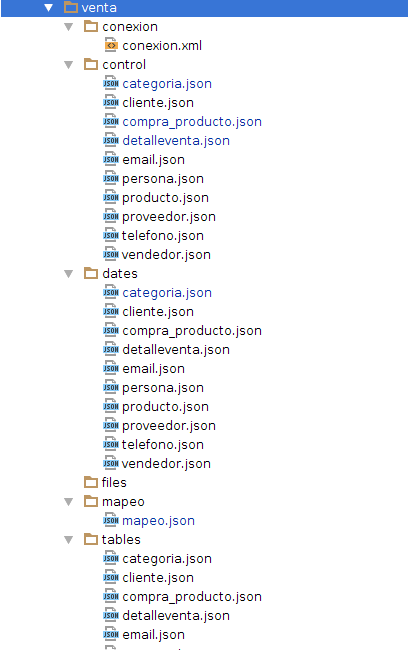
\includegraphics[scale=0.5]{images/estructura.png}
\caption{Estructura}
\label{estructuradirectoriosfiles}
\end{figure}

Donde se guarda la informaci'on de los archivos de configuraci'on, veamos en detalle cada directorio y su contenido:
\begin{itemize}
\item \textbf{conexi\'on} En este directorio se tiene un archivo \textit{conexion.xml} la cual contiene la informaci'on de los datos de conexi'on. Va separada en un directorio por razones de que puede existir un nombre de una tabla igual al archivo por lo que es necesario que no se confunda.
\item \textbf{control} Si se observa el contenido de los directorios \textit{control, dates, tables} son similares la diferencia esta en el contenido de los archivos.
 
En este directorio se almacena archivos de control de las columnas por cada tabla y que tienen el mismo nombre que en la base de datos ver el contenido para la tabla \textit{compra\_producto} de la Figura \ref{fig:Modelo ER} se obtiene informacion como se ve en el c'odigo \ref{jsoncompraproducto}.

\begin{lstlisting}[caption={Ejemplo archivo control},label={jsoncompraproducto},language=sql]
[
  {
    "column_name": "cod_producto",
    "is_nullable": "NO",
    "rellenado": false
  },
  {
    "column_name": "cod_proveedor",
    "is_nullable": "NO",
    "rellenado": false
  },
  {
    "column_name": "cod_compra_producto",
    "is_nullable": "NO",
    "rellenado": false
  },
  {
    "column_name": "fecha_compra_producto",
    "is_nullable": "NO",
    "rellenado": false
  }
]
\end{lstlisting}.
 
Se encuentra informaci\'on en formato JSON clave - valor y donde \textit{column\_name} indica el nombre de la columna, \textit{is\_nullable} indica si este campo puede ser nulo y por ultimo \textit{rellenado} llega a ser la mas importante porque es aqu'i donde controlar si ya fue configurada esta columna.
\item \textbf{dates} los archivos de este directorio almacenan informaci'on generada por cada columna, a excepci'on de tipos de datos como bytea o blob, para este tipo de datos es recomendable almacenar el nombre del archivo. El formato del archivo que almacena la informaci\'on generada es el codigo \ref{jsoncategoria}:
\begin{lstlisting}[caption={Ejemplo archivo dates},label={jsoncategoria},language=sql]
[
  {
    "nombre_categoria": "bebida",
    "cod_categoria": "1"
  },
  {
    "nombre_categoria": "comidarapida",
    "cod_categoria": 2
  },
  {
    "nombre_categoria": "enlatados",
    "cod_categoria": 3
  },
  {
    "nombre_categoria": "especial",
    "cod_categoria": 4
  },
  {
    "nombre_categoria": "ensaladas",
    "cod_categoria": 5
  }
]
\end{lstlisting}
Si se observa la Figura \ref{fig:Modelo ER} la tabla \textit{categoria} tiene dos atributos \textit{nombre\_categoria} y \textit{cod\_categoria}, al ver el contenido del archivo \textit{categoria.json} de directorio \textit{dates} existen varios registros con los valores asignados, la cantidad puede variar dependiendo de la cantidad de datos que se quiere generar.
 \item \textbf{files} En este directorio se almacenan los archivos de tipo bytea y que al momento de hacer la insercion usar por su nombre.
 \item \textbf{mapeo} Solo existe un archivo con un contenido de la lista de las tablas seg'un el orden en que estas deben ser configurados adem'as tiene dos atributos mas \textit{nivel} la cual indica cual es el orden en que le corresponde y por ultimo la \textit{cantidad} si se encuentra un valor igual a cero es porque esta tabla no tiene columna alguna configurada esto deja entender que si se da un valor, es para la tabla en general. Ver para el caso de la Figura \ref{fig:Modelo ER} se tiene la estructura de control como se ve en el codigo \ref{jsonmodelo}.
\begin{lstlisting}[caption={Ejemplo archivo mapeo},label={jsonmodelo},language=sql]
[
  {
    "tablename": "categoria",
    "nivel": 0,
    "cantidad": "5"
  },
  {
    "tablename": "persona",
    "nivel": 0,
    "cantidad": 0
  },
  {
    "tablename": "producto",
    "nivel": 1,
    "cantidad": 0
  },
  .
  .
  .
  {
    "tablename": "compra_producto",
    "nivel": 2,
    "cantidad": 0
  },
  {
    "tablename": "detalleventa",
    "nivel": 2,
    "cantidad": 0
  }
]
\end{lstlisting}  
\item \textbf{tables} En el directorio tables es donde se almaceno la informaci'on detallada por cada una de las tablas, adem'as cada archivo representa a una tabla de la base de datos y que llevan el mismo nombre. Se puede ver el contenido del archivo \textit{categoria.json} en el c'odigo \ref{jsontables} que representa a la tabla \textit{categoria}:

\begin{lstlisting}[caption={Ejemplo archivo tables},label={jsontables},language=sql]
[
  {
    "column_name": "cod_categoria",
    "data_type": "integer",
    "character_maximum_length": null,
    "es_foranea": "false",
    "referencian": null,
    "tabla": null,
    "referenciados": null,
    "numeric_precision": "32",
    "is_nullable": "NO",
    "constraint_type": "PRIMARY KEY",
    "column_default": "nextval('categoria_cod_categoria_seq'::regclass)",
    "check_clause": null
  },
  {
    "column_name": "nombre_categoria",
    "data_type": "character varying",
    "character_maximum_length": null,
    "es_foranea": "false",
    "referencian": null,
    "tabla": null,
    "referenciados": null,
    "numeric_precision": null,
    "is_nullable": "NO",
    "constraint_type": null,
    "column_default": null,
    "check_clause": null
  }
]
\end{lstlisting} 
\end{itemize}

Es una estructura de directorios que no necesariamente se tienen que llamar as'i, sin embargo el nombre de los archivos es aconsejable que lleven el mismo nombre que en la base de datos para que resulte mas amigable.
\section{Configuraci'on de columnas}
Una vez que se tiene el proyecto creado, la configuraci'on que se hace es por cada columna de la tabla para lo cual es necesario saber que tipo de dato acepta cada columna o si hace referencia a otra tabla.
Las columnas de una tabla puede ser de diferente tipo de dato(\textit{integer, varchar, boolean y otros}). Independientemente del tipo de dato de una columna se puede agruparlos tomando en cuenta ciertas caracter'isticas como ser:
\begin{itemize}
\item Que el tipo de dato sea texto, fechas hora, direcciones de red al momento de insertar a la base de datos estos son tomados como si fuesen un texto($'$\textit{valor}$'$).
\item El tipo de dato sea un numero en las que estan (\textit{integer,serial,smallserial,bigserial, beint ...smallint}) est'an son insertados como un numero (\textit{valor}).
\item Que sea una llave primaria sin importar el tipo de dato est'an deben ser 'unicas al momento de generarlos.
\item Cuando sea una llave for'anea no se debe generar por que estas deben existir en la tabla que hace referencia para lo cual se toma los valores generados en la tabla referenciada.
\item El tipo de dato sea bytea es un caso especial que no se trata como una cadena ni como un numero.
\end{itemize}
\subsection{Configuraci'on para llaves for'aneas}
Las llaves for'aneas o primarias que no son propias de la tabla no se necesitan generarlos con un algoritmo, lo que se hace es trabajar con los datos generados en la columna de la tabla al que se hace referencia, En este proyecto la t'ecnica empleada para el manejo de estas fue agruparlos todas las que hacen referencia en conjunto a alguna tabla como si fuese una sola columna a continuaci'on se presenta un ejemplo en la Figura \ref{fig:ejemploForaneasLine}.
\begin{figure}[H]
\centering
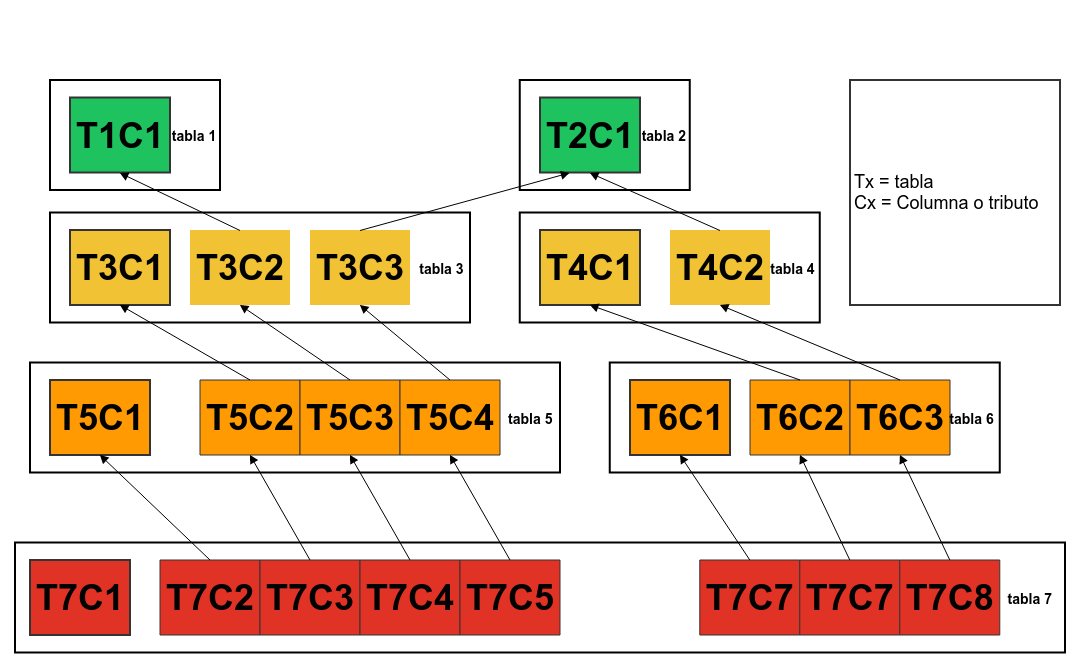
\includegraphics[scale=0.4]{images/foraneasline.png}
\caption{Foraneas line}\label{fig:ejemploForaneasLine}
\end{figure}
Donde la \textit{tabla1} cuenta con una llave primaria (\textit{T1C1})  al igual que la \textit{tabla2}, y si se baja un nivel mas abajo a la \textit{tabla3} esta hace referencia a \textit{tabla1} y \textit{tabla2} y que las columnas de las tablas referenciadas mandan como llaves primarias, formando asi una llave compuesta para \textit{tabla3}. Por otro lado la \textit{tabla4} hace referencia a \textit{tabla2} y que tambien tiene una llave compuesta. Si se baja a la \textit{tabla5} esta compuesta de 4 columnas de las cuales 3 no son propias, si se observa vienen juntadas como si fuera una columna es lo que se hizo al momento de guardar el detalle de una tabla, En la \textit{tabla7} se hace referencia a la \textit{tabla5} y \textit{tabla6} y las columnas que no son propias son agrupadas de acuerdo a que tabla se haga referencia es el caso de \textit{T7C2, T7C3, T7C4, T7C5} que en conjunto hacen referencia a la \textit{tabla5} y \textit{T7C6, T7C7, T7C8} hacen referencia a \textit{tabla6}.

Al momento de hacer la configuraci\'on se llega a tener un problema, de la \textit{tabla5} el campo  \textit{T5C2, T5C3, T5C4} no es encontrada si se lo busca como una columna en la \textit{tabla3} como es posible si se tiene esas columnas? Es cierto que existen pero est'an separadas como se observa en la Figura \ref{fig:problemaColumnasForaneasLine}.
\begin{figure}[H]
\centering
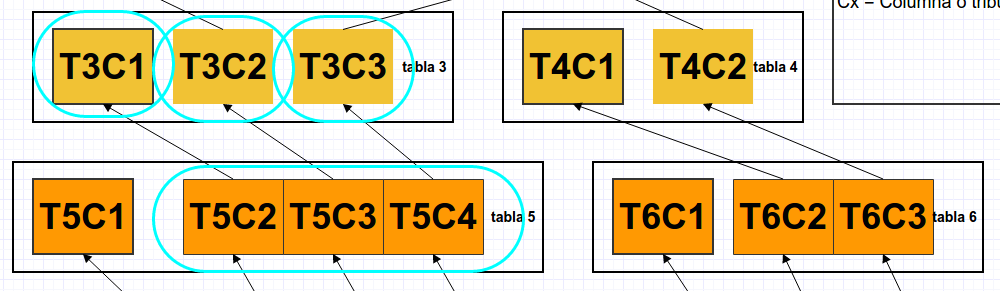
\includegraphics[scale=0.4]{images/problemaColumnas.png}
\caption{Problema llaves foraneas}\label{fig:problemaColumnasForaneasLine}
\end{figure}
Se da el mismo problema para la \textit{tabla7} la columna \textit{T7C2, T7C3, T7C4, T7C5} no se encuentra en una solo columna en la \textit{tabla5} pero hay algo interesante que se puede deducir como se observa en la Figura \ref{fig:problemaColumnasForaneasGrafica}.
\begin{figure}[H]
\centering
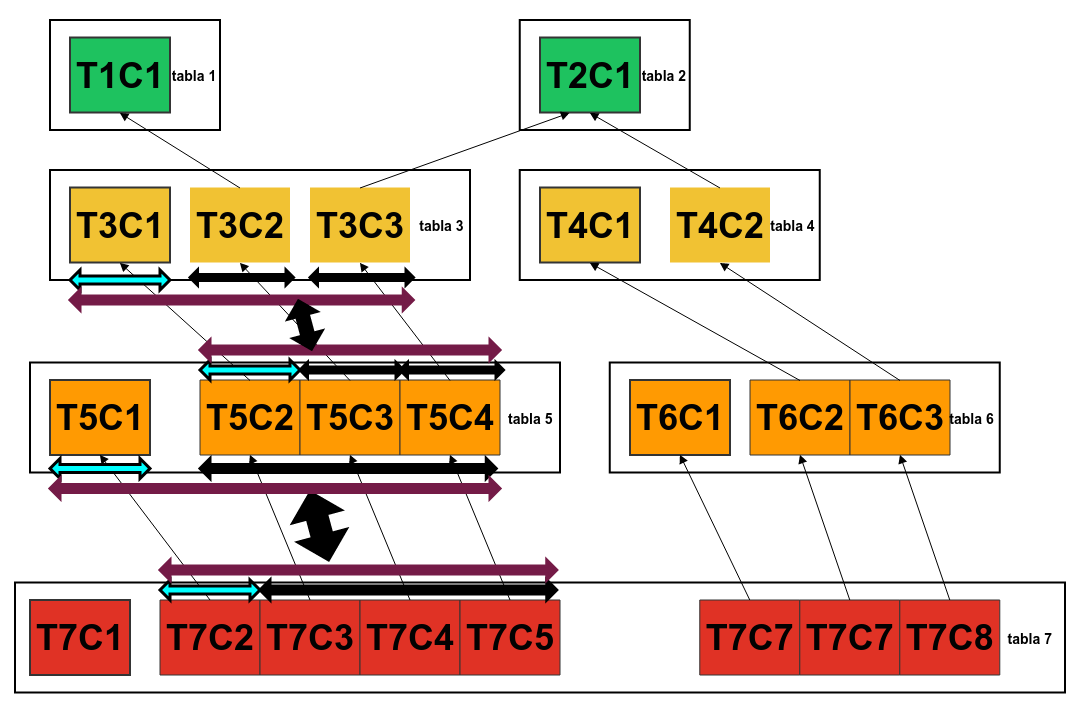
\includegraphics[scale=0.3]{images/problemaForaneas.png}
\caption{Ejemplo foraneas unidas}\label{fig:problemaColumnasForaneasGrafica}
\end{figure}
En la \textit{tabla5} las columnas \textit{T5C2, T5C3, T5C4} en conjunto hacen referencia como una sola a la \textit{tabla3} donde \textit{T5C2} apunta a \textit{T3C1} y que esta es una llave primaria propia de la \textit{tabla3}, en la \textit{tabla7} la columna  \textit{T7C2} hace referencia a una propia de la \textit{tabla5}, se puede determinar que el comportamiento de las llaves primarias que no son propias siguen este modelo.
\subsubsection{Problemas}
El problema surge al momento de realizar la validaci\'on que por ejemplo cuando por alguna raz\'on se trata de configurar un atributo que hace referencia y que previamente no se configuraci\'on los atributos referenciados en la tabla referenciada no se llega a encontrar como se ve en la figura \ref{fig:problemaColumnasForaneasGrafica}. Las columnas de la \textit{tabla3} se va encontrar todas al igual que en la \textit{tabla4}, pero en la \textit{tabla5} no se llega a encontrar la columna \textit{T5C2T5C3T5C4} lo mismo sucede con \textit{T6C2T6C3}.
Una vez hecha la validaci\'on el siguiente paso es configurar, para lo cual se necesita los datos de la tabla referenciada, al fijarse en la Figura \ref{fig:problemaColumnasForaneasGrafica} se encuentra en el mismo problema de la validaci\'on de columnas no encontradas.   
\subsubsection{Soluciones}
Una soluci\'on obvia al problema de la validaci\'on presentado es verificar que todas las columnas de la tabla referenciada se encuentren configuradas para no tener problemas al obtener los datos pero no es tan cierto se puede configurar con solo tener configuradas las columnas referenciadas se puede optar por cualquiera son cuestiones de validaci\'on.

En cuanto al problema de la configuraci\'on una vez pasada la anterior la soluci\'on no llega a ser tan sencilla se necesita aplicar algun mecanismo(os) de obtener los datos. La soluci\'on que se da no estrictamente depende del modelo y del manejo de iniciar con la Figura \ref{intento1}.
\begin{figure}[H]
\centering
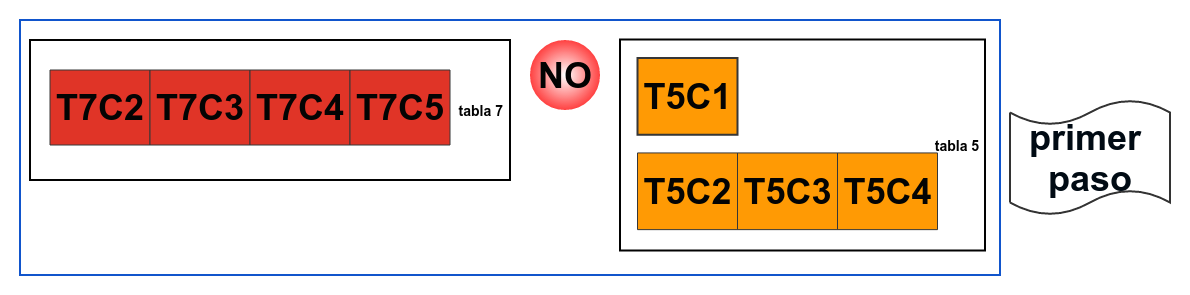
\includegraphics[scale=0.35]{images/paso1.png}
\caption{primer intento}\label{intento1}
\end{figure}
En el primer intento no se llega a la soluci\'on ya que no se encuentra la columna en la \textit{tabla5}, pasar a observar a la Figura \ref{intento2}.
\begin{figure}[H]
\centering
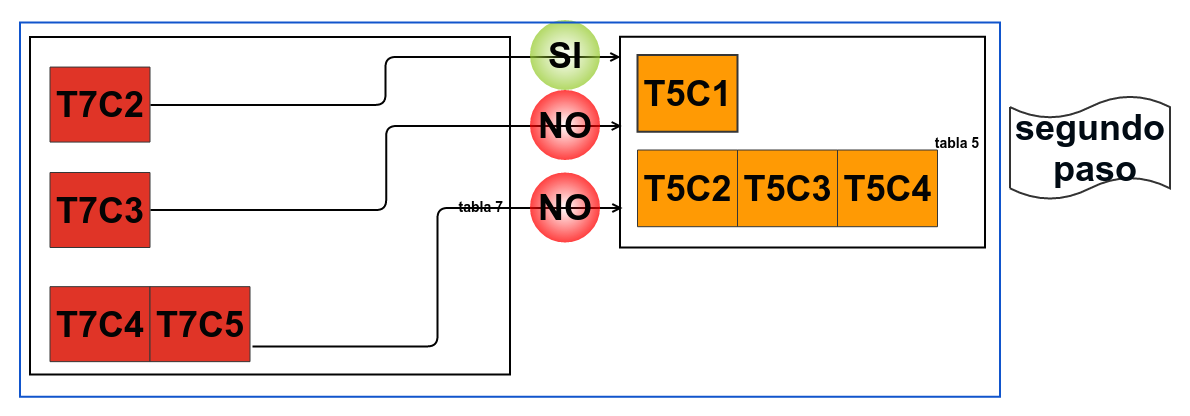
\includegraphics[scale=0.35]{images/paso2.png}
\caption{segundo intento}\label{intento2}
\end{figure}
Iniciar con el primer elemento buscando en la tabla referenciada en caso de que exista pasar al siguiente elemento caso contrario listar en una lista de los elementos no encontrados, pasar a ver la Figura \ref{intento3}. 
\begin{figure}[H]
\centering
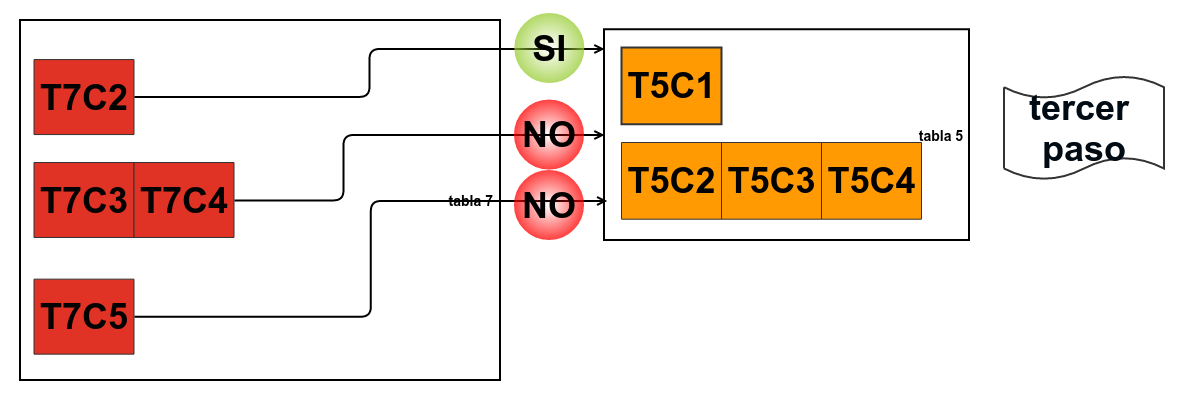
\includegraphics[scale=0.35]{images/paso3.png}
\caption{tercer intento}\label{intento3}
\end{figure}
Pasar con el siguiente elemento uniendo con las no encontradas y se vuelve a buscar en la tabla referenciada como aun no se encontro pasar al siguiente como se observa en la Figura \ref{intento4}.
\begin{figure}[H]
\centering
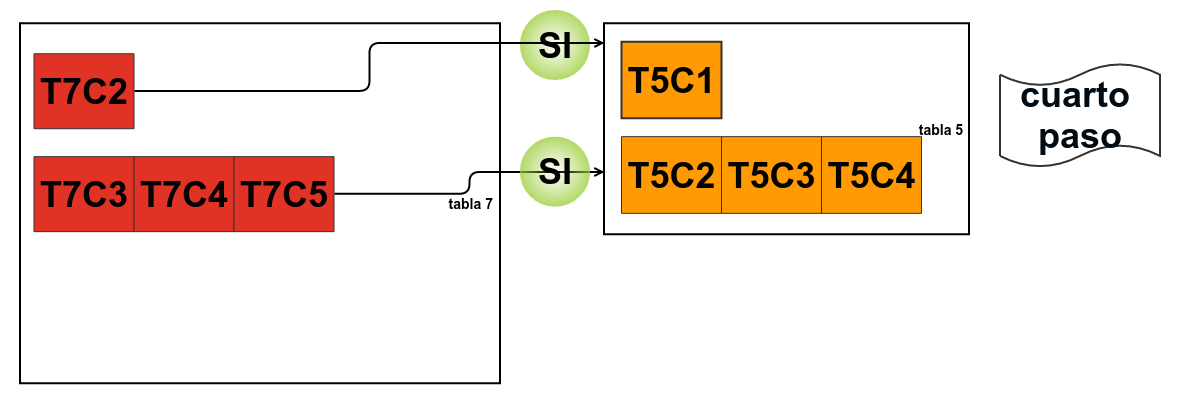
\includegraphics[scale=0.35]{images/paso4.png}
\caption{cuarto intento}\label{intento4}
\end{figure}
En este paso se vuelve a juntar las no encontradas y el elemento a obtener y buscar en la tabla referenciada y como se encontro y no hay mas elementos que buscar se llega a la soluci\'on.
\chapter{Crear proyecto de configuraci'on}

Cuando se realiza el llenado de datos de prueba sobre una base de datos, hay un inicio y un final donde no siempre se inicia y acaba sin alguna interrupci'on, por muchas razones fallas el'ectricas, cansancio entre otras, para lo cual es importante que toda la informaci'on obtenida en el capitulo anterior sea persistente y que sea posible tener esa informaci'on sin volver a ejecutar los algoritmos adem'as sin la necesidad de volver a conectar a la base de datos.
Para lo cual se almacena en archivos de texto plano con alg'un formato, entre los formatos mas conocidos se tiene a XML (Extensible Markup Language o Lenguaje de Marcas Extensible) y JSON (JavaScript Object Notation - Notaci\'on de Objetos de JavaScript).

\section{JSON (JavaScript Object Notation - Notaci\'on de Objetos de JavaScript)}
Es un formato ligero de intercambio de datos. Leerlo y escribirlo es simple para humanos, mientras que para las m\'aquinas es simple interpretarlo y generarlo. Est\'a basado en un subconjunto del Lenguaje de Programaci\'on JavaScript, Standard ECMA-262 3rd Edition - Diciembre 1999. JSON es un formato de texto que es completamente independiente del lenguaje pero utiliza convenciones que son ampliamente conocidos por los programadores de la familia de lenguajes C, incluyendo C, C++, C\#, Java, JavaScript, Perl, Python, y muchos otros. Estas propiedades hacen que JSON sea un lenguaje ideal para el intercambio de datos.
JSON está constituido por dos estructuras:

\begin{itemize}
\item Una colecci\'on de pares de nombre/valor. En varios lenguajes esto es conocido como un objeto, registro, estructura, diccionario, tabla hash, lista de claves o un arreglo asociativo.
\item Una lista ordenada de valores. En la mayor\'ia de los lenguajes, esto se implementa como arreglos, vectores, listas o secuencias.
\end{itemize}

Estas son estructuras universales; virtualmente todos los lenguajes de programaci\'on las soportan de una forma u otra. Es razonable que un formato de intercambio de datos que es independiente del lenguaje de programaci\'on se base en estas estructuras.

En JSON, se presentan de estas formas:


Un objeto es un conjunto desordenado de pares nombre/valor como se ve en la Figura \ref{fig:objectJSON}. Un objeto comienza con { (llave de apertura) y termine con } (llave de cierre). Cada nombre es seguido por : (dos puntos) y los pares nombre/valor están separados por (coma).
\begin{figure}[H]
\centering
\subfigure{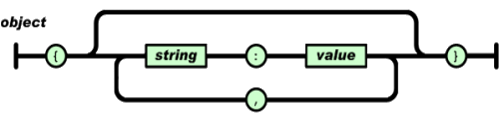
\includegraphics[width=120mm,height=25mm]{images/objectJSON}}
\caption{Object JSON} \label{fig:objectJSON}
\end{figure}

Un arreglo es una colecci\'on de valores. Un arreglo comienza con [ (corchete izquierdo) y termina con ] (corchete derecho) como se ve en la Figura \ref{fig:arrayJSON}. Los valores se separan por , (coma).

\begin{figure}[H]
\centering
\subfigure{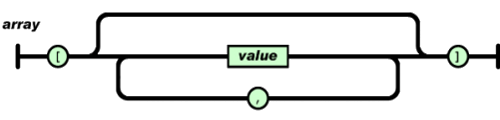
\includegraphics[width=120mm,height=25mm]{images/arrayJSON}}
\caption{Array JSON} \label{fig:arrayJSON}
\end{figure}

Un valor puede ser una cadena de caracteres con comillas dobles, o un n\'umero, o true o false o null, o un objeto o un arreglo como se observa en la Figura \ref{fig:valueJSON}. Estas estructuras pueden anidar

\begin{figure}[H]
\centering
\subfigure{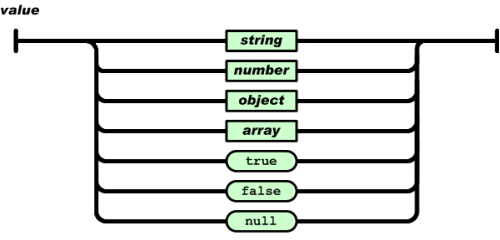
\includegraphics[width=120mm,height=65mm]{images/valueJSON}}
\caption{Value JSON} \label{fig:valueJSON}
\end{figure}

Una cadena de caracteres es una colecci\'on de cero o m\'as caracteres Unicode, encerrados entre comillas dobles, usando barras divisorias invertidas como escape. Un car\'acter est\'a representado por una cadena de caracteres de un \'unico car\'acter ver Figura \ref{fig:stringJSON}. Una cadena de caracteres es parecida a una cadena de caracteres C o Java.

\begin{figure}[H]
\centering
\subfigure{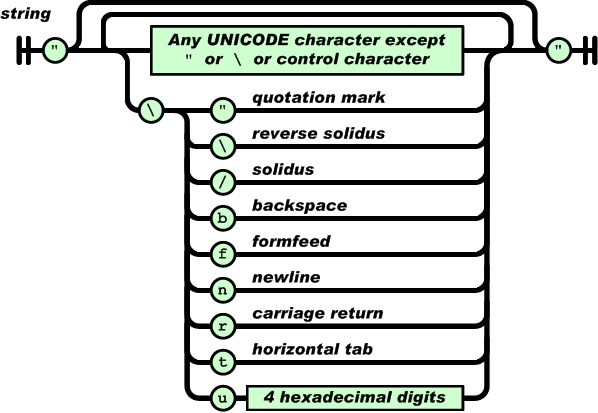
\includegraphics[width=120mm,height=60mm]{images/stringJSON}}
\caption{String JSON} \label{fig:stringJSON}
\end{figure}

Un n\'umero es similar a un n\'umero C o Java, excepto que no se usan los formatos octales y hexadecimales ver la Figura \ref{fig:numberJSON}.

\begin{figure}[H]
\centering
\subfigure{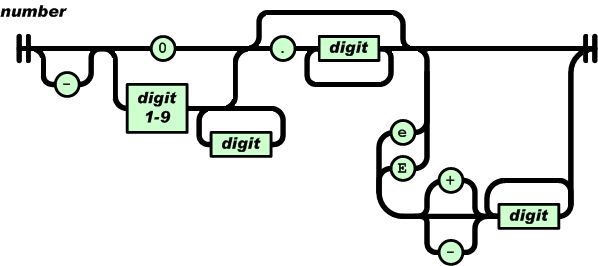
\includegraphics[width=120mm,height=50mm]{images/numberJSON}}
\caption{Number JSON} \label{fig:numberJSON}
\end{figure}

Los espacios en blanco pueden insertarse entre cualquier par de s\'imbolos.

\section{Persistencia de la informaci\'on de metadatos}
La informaci\'on obtenida en el anterior capitulo es necesario que sean persistentes para la reanudaci\'on  en el proceso de configuraci\'on para el objetivo, la informaci'on necesaria a persistir son las siguientes:
\begin{itemize}
\item Datos de la conexi\'on a la base de datos como ser el nombre de la base de datos, usuario, contrase\~na, puerto y el host.
\item La lista de las tablas de la base de datos elegida seg'un al orden en que estos deben ser llenados que se obtuvo en el capitulo anterior.
\item El detalle por cada una de las tablas (nombre de la columna, el tipo de dato, si acepta que sea nulo, si es una llave etc...).  
\end{itemize}
Una alternativa para dar soluci\'on a este requisito es almacenar toda esta informaci'on en archivos sea en el formato JSON o XML, en este proyecto se optar\'a por Json las razones son las siguientes:

\begin{itemize}
\item Soporta dos tipos de estructuras, una de ellas son objetos que contienen una colecci\'on de pares llave-valor y el otro tipo se trata de arrays de valores. Esto proporciona una gran sencillez en las estructuras.
\item No tiene espacios de nombres, cada objeto es un conjunto de claves independientes de cualquier otro objeto.
\item JSON no necesita ser extensible por que es flexible por s\'i solo. Puede representar cualquier estructura de datos pudiendo a\~nadir nuevos campos con total facilidad.
\item Es mucho mas simple que XML, el cual proporciona pesadas tecnolog\'ias que le avalan (Scheme, XSLT, XPath).
\item Si se compara el tama\~no de un archivo JSON con uno XML y que contenga la misma informaci\'on el primero llega a ser mucho mas peque\~no.
\end{itemize} 
\subsection{Creando la estructura de un proyecto}
Cuando sea crea un proyecto java, php, python u otro, normalmente se tiene un estructura de directorios y archivos, donde ciertos archivos guardan configuraciones sobre recursos que se hacen uso, la version del proyecto entre otros. Para este proyecto se realiza algo similar para lo cual se va tener como base la estructura de la Figura \ref{estructuradirectoriosfiles} de directorios y archivos.

\begin{figure}[H]
\centering
\includegraphics[scale=0.5]{images/estructura.png}
\caption{Estructura}
\label{estructuradirectoriosfiles}
\end{figure}

Donde se guarda la informaci'on de los archivos de configuraci'on, veamos en detalle cada directorio y su contenido:
\begin{itemize}
\item \textbf{conexi\'on} En este directorio se tiene un archivo \textit{conexion.xml} la cual contiene la informaci'on de los datos de conexi'on. Va separada en un directorio por razones de que puede existir un nombre de una tabla igual al archivo por lo que es necesario que no se confunda.
\item \textbf{control} Si se observa el contenido de los directorios \textit{control, dates, tables} son similares la diferencia esta en el contenido de los archivos.
 
En este directorio se almacena archivos de control de las columnas por cada tabla y que tienen el mismo nombre que en la base de datos ver el contenido para la tabla \textit{compra\_producto} de la Figura \ref{fig:Modelo ER} se obtiene informacion como se ve en el c'odigo \ref{jsoncompraproducto}.

\begin{lstlisting}[caption={Ejemplo archivo control},label={jsoncompraproducto},language=sql]
[
  {
    "column_name": "cod_producto",
    "is_nullable": "NO",
    "rellenado": false
  },
  {
    "column_name": "cod_proveedor",
    "is_nullable": "NO",
    "rellenado": false
  },
  {
    "column_name": "cod_compra_producto",
    "is_nullable": "NO",
    "rellenado": false
  },
  {
    "column_name": "fecha_compra_producto",
    "is_nullable": "NO",
    "rellenado": false
  }
]
\end{lstlisting}.
 
Se encuentra informaci\'on en formato JSON clave - valor y donde \textit{column\_name} indica el nombre de la columna, \textit{is\_nullable} indica si este campo puede ser nulo y por ultimo \textit{rellenado} llega a ser la mas importante porque es aqu'i donde controlar si ya fue configurada esta columna.
\item \textbf{dates} los archivos de este directorio almacenan informaci'on generada por cada columna, a excepci'on de tipos de datos como bytea o blob, para este tipo de datos es recomendable almacenar el nombre del archivo. El formato del archivo que almacena la informaci\'on generada es el codigo \ref{jsoncategoria}:
\begin{lstlisting}[caption={Ejemplo archivo dates},label={jsoncategoria},language=sql]
[
  {
    "nombre_categoria": "bebida",
    "cod_categoria": "1"
  },
  {
    "nombre_categoria": "comidarapida",
    "cod_categoria": 2
  },
  {
    "nombre_categoria": "enlatados",
    "cod_categoria": 3
  },
  {
    "nombre_categoria": "especial",
    "cod_categoria": 4
  },
  {
    "nombre_categoria": "ensaladas",
    "cod_categoria": 5
  }
]
\end{lstlisting}
Si se observa la Figura \ref{fig:Modelo ER} la tabla \textit{categoria} tiene dos atributos \textit{nombre\_categoria} y \textit{cod\_categoria}, al ver el contenido del archivo \textit{categoria.json} de directorio \textit{dates} existen varios registros con los valores asignados, la cantidad puede variar dependiendo de la cantidad de datos que se quiere generar.
 \item \textbf{files} En este directorio se almacenan los archivos de tipo bytea y que al momento de hacer la insercion usar por su nombre.
 \item \textbf{mapeo} Solo existe un archivo con un contenido de la lista de las tablas seg'un el orden en que estas deben ser configurados adem'as tiene dos atributos mas \textit{nivel} la cual indica cual es el orden en que le corresponde y por ultimo la \textit{cantidad} si se encuentra un valor igual a cero es porque esta tabla no tiene columna alguna configurada esto deja entender que si se da un valor, es para la tabla en general. Ver para el caso de la Figura \ref{fig:Modelo ER} se tiene la estructura de control como se ve en el codigo \ref{jsonmodelo}.
\begin{lstlisting}[caption={Ejemplo archivo mapeo},label={jsonmodelo},language=sql]
[
  {
    "tablename": "categoria",
    "nivel": 0,
    "cantidad": "5"
  },
  {
    "tablename": "persona",
    "nivel": 0,
    "cantidad": 0
  },
  {
    "tablename": "producto",
    "nivel": 1,
    "cantidad": 0
  },
  .
  .
  .
  {
    "tablename": "compra_producto",
    "nivel": 2,
    "cantidad": 0
  },
  {
    "tablename": "detalleventa",
    "nivel": 2,
    "cantidad": 0
  }
]
\end{lstlisting}  
\item \textbf{tables} En el directorio tables es donde se almaceno la informaci'on detallada por cada una de las tablas, adem'as cada archivo representa a una tabla de la base de datos y que llevan el mismo nombre. Se puede ver el contenido del archivo \textit{categoria.json} en el c'odigo \ref{jsontables} que representa a la tabla \textit{categoria}:

\begin{lstlisting}[caption={Ejemplo archivo tables},label={jsontables},language=sql]
[
  {
    "column_name": "cod_categoria",
    "data_type": "integer",
    "character_maximum_length": null,
    "es_foranea": "false",
    "referencian": null,
    "tabla": null,
    "referenciados": null,
    "numeric_precision": "32",
    "is_nullable": "NO",
    "constraint_type": "PRIMARY KEY",
    "column_default": "nextval('categoria_cod_categoria_seq'::regclass)",
    "check_clause": null
  },
  {
    "column_name": "nombre_categoria",
    "data_type": "character varying",
    "character_maximum_length": null,
    "es_foranea": "false",
    "referencian": null,
    "tabla": null,
    "referenciados": null,
    "numeric_precision": null,
    "is_nullable": "NO",
    "constraint_type": null,
    "column_default": null,
    "check_clause": null
  }
]
\end{lstlisting} 
\end{itemize}

Es una estructura de directorios que no necesariamente se tienen que llamar as'i, sin embargo el nombre de los archivos es aconsejable que lleven el mismo nombre que en la base de datos para que resulte mas amigable.
\section{Configuraci'on de columnas}
Una vez que se tiene el proyecto creado, la configuraci'on que se hace es por cada columna de la tabla para lo cual es necesario saber que tipo de dato acepta cada columna o si hace referencia a otra tabla.
Las columnas de una tabla puede ser de diferente tipo de dato(\textit{integer, varchar, boolean y otros}). Independientemente del tipo de dato de una columna se puede agruparlos tomando en cuenta ciertas caracter'isticas como ser:
\begin{itemize}
\item Que el tipo de dato sea texto, fechas hora, direcciones de red al momento de insertar a la base de datos estos son tomados como si fuesen un texto($'$\textit{valor}$'$).
\item El tipo de dato sea un numero en las que estan (\textit{integer,serial,smallserial,bigserial, beint ...smallint}) est'an son insertados como un numero (\textit{valor}).
\item Que sea una llave primaria sin importar el tipo de dato est'an deben ser 'unicas al momento de generarlos.
\item Cuando sea una llave for'anea no se debe generar por que estas deben existir en la tabla que hace referencia para lo cual se toma los valores generados en la tabla referenciada.
\item El tipo de dato sea bytea es un caso especial que no se trata como una cadena ni como un numero.
\end{itemize}
\subsection{Configuraci'on para llaves for'aneas}
Las llaves for'aneas o primarias que no son propias de la tabla no se necesitan generarlos con un algoritmo, lo que se hace es trabajar con los datos generados en la columna de la tabla al que se hace referencia, En este proyecto la t'ecnica empleada para el manejo de estas fue agruparlos todas las que hacen referencia en conjunto a alguna tabla como si fuese una sola columna a continuaci'on se presenta un ejemplo en la Figura \ref{fig:ejemploForaneasLine}.
\begin{figure}[H]
\centering
\includegraphics[scale=0.4]{images/foraneasline.png}
\caption{Foraneas line}\label{fig:ejemploForaneasLine}
\end{figure}
Donde la \textit{tabla1} cuenta con una llave primaria (\textit{T1C1})  al igual que la \textit{tabla2}, y si se baja un nivel mas abajo a la \textit{tabla3} esta hace referencia a \textit{tabla1} y \textit{tabla2} y que las columnas de las tablas referenciadas mandan como llaves primarias, formando asi una llave compuesta para \textit{tabla3}. Por otro lado la \textit{tabla4} hace referencia a \textit{tabla2} y que tambien tiene una llave compuesta. Si se baja a la \textit{tabla5} esta compuesta de 4 columnas de las cuales 3 no son propias, si se observa vienen juntadas como si fuera una columna es lo que se hizo al momento de guardar el detalle de una tabla, En la \textit{tabla7} se hace referencia a la \textit{tabla5} y \textit{tabla6} y las columnas que no son propias son agrupadas de acuerdo a que tabla se haga referencia es el caso de \textit{T7C2, T7C3, T7C4, T7C5} que en conjunto hacen referencia a la \textit{tabla5} y \textit{T7C6, T7C7, T7C8} hacen referencia a \textit{tabla6}.

Al momento de hacer la configuraci\'on se llega a tener un problema, de la \textit{tabla5} el campo  \textit{T5C2, T5C3, T5C4} no es encontrada si se lo busca como una columna en la \textit{tabla3} como es posible si se tiene esas columnas? Es cierto que existen pero est'an separadas como se observa en la Figura \ref{fig:problemaColumnasForaneasLine}.
\begin{figure}[H]
\centering
\includegraphics[scale=0.4]{images/problemaColumnas.png}
\caption{Problema llaves foraneas}\label{fig:problemaColumnasForaneasLine}
\end{figure}
Se da el mismo problema para la \textit{tabla7} la columna \textit{T7C2, T7C3, T7C4, T7C5} no se encuentra en una solo columna en la \textit{tabla5} pero hay algo interesante que se puede deducir como se observa en la Figura \ref{fig:problemaColumnasForaneasGrafica}.
\begin{figure}[H]
\centering
\includegraphics[scale=0.3]{images/problemaForaneas.png}
\caption{Ejemplo foraneas unidas}\label{fig:problemaColumnasForaneasGrafica}
\end{figure}
En la \textit{tabla5} las columnas \textit{T5C2, T5C3, T5C4} en conjunto hacen referencia como una sola a la \textit{tabla3} donde \textit{T5C2} apunta a \textit{T3C1} y que esta es una llave primaria propia de la \textit{tabla3}, en la \textit{tabla7} la columna  \textit{T7C2} hace referencia a una propia de la \textit{tabla5}, se puede determinar que el comportamiento de las llaves primarias que no son propias siguen este modelo.
\subsubsection{Problemas}
El problema surge al momento de realizar la validaci\'on que por ejemplo cuando por alguna raz\'on se trata de configurar un atributo que hace referencia y que previamente no se configuraci\'on los atributos referenciados en la tabla referenciada no se llega a encontrar como se ve en la figura \ref{fig:problemaColumnasForaneasGrafica}. Las columnas de la \textit{tabla3} se va encontrar todas al igual que en la \textit{tabla4}, pero en la \textit{tabla5} no se llega a encontrar la columna \textit{T5C2T5C3T5C4} lo mismo sucede con \textit{T6C2T6C3}.
Una vez hecha la validaci\'on el siguiente paso es configurar, para lo cual se necesita los datos de la tabla referenciada, al fijarse en la Figura \ref{fig:problemaColumnasForaneasGrafica} se encuentra en el mismo problema de la validaci\'on de columnas no encontradas.   
\subsubsection{Soluciones}
Una soluci\'on obvia al problema de la validaci\'on presentado es verificar que todas las columnas de la tabla referenciada se encuentren configuradas para no tener problemas al obtener los datos pero no es tan cierto se puede configurar con solo tener configuradas las columnas referenciadas se puede optar por cualquiera son cuestiones de validaci\'on.

En cuanto al problema de la configuraci\'on una vez pasada la anterior la soluci\'on no llega a ser tan sencilla se necesita aplicar algun mecanismo(os) de obtener los datos. La soluci\'on que se da no estrictamente depende del modelo y del manejo de iniciar con la Figura \ref{intento1}.
\begin{figure}[H]
\centering
\includegraphics[scale=0.35]{images/paso1.png}
\caption{primer intento}\label{intento1}
\end{figure}
En el primer intento no se llega a la soluci\'on ya que no se encuentra la columna en la \textit{tabla5}, pasar a observar a la Figura \ref{intento2}.
\begin{figure}[H]
\centering
\includegraphics[scale=0.35]{images/paso2.png}
\caption{segundo intento}\label{intento2}
\end{figure}
Iniciar con el primer elemento buscando en la tabla referenciada en caso de que exista pasar al siguiente elemento caso contrario listar en una lista de los elementos no encontrados, pasar a ver la Figura \ref{intento3}. 
\begin{figure}[H]
\centering
\includegraphics[scale=0.35]{images/paso3.png}
\caption{tercer intento}\label{intento3}
\end{figure}
Pasar con el siguiente elemento uniendo con las no encontradas y se vuelve a buscar en la tabla referenciada como aun no se encontro pasar al siguiente como se observa en la Figura \ref{intento4}.
\begin{figure}[H]
\centering
\includegraphics[scale=0.35]{images/paso4.png}
\caption{cuarto intento}\label{intento4}
\end{figure}
En este paso se vuelve a juntar las no encontradas y el elemento a obtener y buscar en la tabla referenciada y como se encontro y no hay mas elementos que buscar se llega a la soluci\'on.
%\chapter{Poblando datos en la base de datos y probando el comportamiento}
Una vez que se tiene configurada en forma completa un proyecto, el siguiente proceso a realizar es el poblado de datos y posteriormente realizar algunas consultas de prueba para ver el comportamiento con una poblaci'on de datos mayor. Para llevar adelante este objetivo es necesario tener la siguiente informaci'on. 
\begin{itemize}
\item Recuperar datos de conexi'on para la base de datos y realizar la conexi'on.
\item Obtener los datos de archivo \textit{mapeo.json} donde se encuentra el orden de las tablas.
\item Por cada tabla crear la estructura SQL de inserci'on \texttt{INSERT INTO tabla (col1,col2...coln)VALUES (val1,val2...valn)}.

Existe casos muy importantes al crear la estructura de datos, la cantidad de columnas que tiene una tabla, el tipo de dato de cada columna, al momento de hacer la inserci'on es importante tomar en cuenta estos casos , la insercion varia dependiendo el tipo de dato.   
\end{itemize} 
\section{Poblado de datos a la base de datos}
Los distintos tipos de datos que provee los DBMS, algunos con una cantidad mayor de tipos de dato y otras con una cantidad mas reducida, es importante analizar como se hara la inserci'on seg'un al tipo de dato, adem'as se debe tomar encuenta la cantidad de columnas que tiene una tabla.
\subsection{Tipos de datos tratados como texto}
Los tipos de datos tratados como cadenas de texto son:
\begin{itemize}
\item Las fechas y horas \texttt{(DATE,DATETIME,TIME)}.
\item Las cadenas de texto \texttt{(VARCHAR,CHARACTER VARYIN,TEXT)}.
\item Las direcciones de red \texttt{(MACADDRESS,INET)}.
\end{itemize}
Estos tipos de datos van entre comillas simples(\texttt{INTO tabla(col)VALUES(`col')}).
\subsection{Tipos de datos tratados como n'umeros}
Los tipos de datos son tratado como un numero entero sea decimal flotante son los tipos de dato como:
\begin{itemize}
\item Los tipos enteros \texttt{(INTEGER, BEGINT, SMALLINT, SERIAL, BIGSERIAL)}.
\item Los tipos decimales \texttt{(FLOAT, DECIMAL MONEY)}.
\end{itemize}
Los tipos de datos num'ericos a diferencia del anterior no van entre comillas(\texttt{INTO tabla(col)VALUES(val)}).
Existe otro tipo de dato mas que se puede incorporar es el tipo \texttt{BOOLEANO} si bien no es un n'umero esta no necesita ir dentro las comillas.
\subsection{Tipo de dato bytea}
El tipo de dato bytea es un tipo especial ya que nececita una conversion previa a la inserci'on, las distintas tecnologias ya se php, java , python , ruby etc... proveen metodos para realizar esta conversi'on, por lo cual no es un tema de preocupaci'on. Si se recuerda al momento de generar los datos el tipo de dato bytea no lo se lo guarda en el archivo generado solo el nombre del archivo, con la que se forma un codigo \texttt{SQL} de insercion de la siguente manera (\texttt{INTO tabla(col)VALUES(conversionprevia(nombre archivo))}).
\subsection{Cantidad de columnas por tabla}
La cantidad de columnas de una tabla es variable, pudiendo tener una o mas columnas para formar la estructura del comando \texttt{INSERT} es necesario obtener la informaci'on del directorio \textit{tables}. Donde cada tabla es representada por un archivo con el mismo nombre de la tabla y que adem'as esta contiene toda la informaci'on detallada de la tabla, entre ellas esta los nombre de las columnas.
Con esta informacion se forma la parte necesaria del comando \texttt{INSERT INTO tabla(col1, col2,...coln)VALUES()}.
En la parte de los valores obtener la informaci'on del directorio \textit{dates del proyecto} y referencia \cite{emifpgsql}.

     
\chapter{Poblando datos en la base de datos y probando el comportamiento}
Una vez que se tiene configurada en forma completa un proyecto, el siguiente proceso a realizar es el poblado de datos y posteriormente realizar algunas consultas de prueba para ver el comportamiento con una poblaci'on de datos mayor. Para llevar adelante este objetivo es necesario tener la siguiente informaci'on. 
\begin{itemize}
\item Recuperar datos de conexi'on para la base de datos y realizar la conexi'on.
\item Obtener los datos de archivo \textit{mapeo.json} donde se encuentra el orden de las tablas.
\item Por cada tabla crear la estructura SQL de inserci'on \texttt{INSERT INTO tabla (col1,col2...coln)VALUES (val1,val2...valn)}.

Existe casos muy importantes al crear la estructura de datos, la cantidad de columnas que tiene una tabla, el tipo de dato de cada columna, al momento de hacer la inserci'on es importante tomar en cuenta estos casos , la insercion varia dependiendo el tipo de dato.   
\end{itemize} 
\section{Poblado de datos a la base de datos}
Los distintos tipos de datos que provee los DBMS, algunos con una cantidad mayor de tipos de dato y otras con una cantidad mas reducida, es importante analizar como se hara la inserci'on seg'un al tipo de dato, adem'as se debe tomar encuenta la cantidad de columnas que tiene una tabla.
\subsection{Tipos de datos tratados como texto}
Los tipos de datos tratados como cadenas de texto son:
\begin{itemize}
\item Las fechas y horas \texttt{(DATE,DATETIME,TIME)}.
\item Las cadenas de texto \texttt{(VARCHAR,CHARACTER VARYIN,TEXT)}.
\item Las direcciones de red \texttt{(MACADDRESS,INET)}.
\end{itemize}
Estos tipos de datos van entre comillas simples(\texttt{INTO tabla(col)VALUES(`col')}).
\subsection{Tipos de datos tratados como n'umeros}
Los tipos de datos son tratado como un numero entero sea decimal flotante son los tipos de dato como:
\begin{itemize}
\item Los tipos enteros \texttt{(INTEGER, BEGINT, SMALLINT, SERIAL, BIGSERIAL)}.
\item Los tipos decimales \texttt{(FLOAT, DECIMAL MONEY)}.
\end{itemize}
Los tipos de datos num'ericos a diferencia del anterior no van entre comillas(\texttt{INTO tabla(col)VALUES(val)}).
Existe otro tipo de dato mas que se puede incorporar es el tipo \texttt{BOOLEANO} si bien no es un n'umero esta no necesita ir dentro las comillas.
\subsection{Tipo de dato bytea}
El tipo de dato bytea es un tipo especial ya que nececita una conversion previa a la inserci'on, las distintas tecnologias ya se php, java , python , ruby etc... proveen metodos para realizar esta conversi'on, por lo cual no es un tema de preocupaci'on. Si se recuerda al momento de generar los datos el tipo de dato bytea no lo se lo guarda en el archivo generado solo el nombre del archivo, con la que se forma un codigo \texttt{SQL} de insercion de la siguente manera (\texttt{INTO tabla(col)VALUES(conversionprevia(nombre archivo))}).
\subsection{Cantidad de columnas por tabla}
La cantidad de columnas de una tabla es variable, pudiendo tener una o mas columnas para formar la estructura del comando \texttt{INSERT} es necesario obtener la informaci'on del directorio \textit{tables}. Donde cada tabla es representada por un archivo con el mismo nombre de la tabla y que adem'as esta contiene toda la informaci'on detallada de la tabla, entre ellas esta los nombre de las columnas.
Con esta informacion se forma la parte necesaria del comando \texttt{INSERT INTO tabla(col1, col2,...coln)VALUES()}.
En la parte de los valores obtener la informaci'on del directorio \textit{dates del proyecto} y referencia \cite{emifpgsql}.

     
%\chapter{uso del prototipo}
En este cap\'itulo hacemos uso del prototipo desarrollado para el poblado de datos de prueba para una base de datos, para lo cual es necesario que se tenga cantidad de tablas.
Como ejemplo tomamos  una base de datos denominada prueba como observamos en la Figura \ref{fig:createDatabase}

\begin{figure}[H]
\caption{base de datos prueba} \label{fig:createDatabase}
\centering
\subfigure{\includegraphics[scale=0.3]{images/prototipo/0-createDatabase.png}}
\end{figure}

Esta base de datos se tiene veinte y dos tablas como se observa en la Figura \ref{fig:listatablePrueba}. 
\begin{figure}[H]
\caption{base de datos prueba} \label{fig:listatablePrueba}
\centering
\subfigure{\includegraphics[scale=0.3]{images/prototipo/1-listTables.png}}
\end{figure}

En el prototipo se tiene la opci\'on de crear como un proyecto en el boton nuevo y la lista de proyectos como se ve en la Figura \ref{fig:homePototype}.
\begin{figure}[H]
\caption{lista de proyectos} \label{fig:homePototype}
\centering
\subfigure{\includegraphics[scale=0.3]{images/prototipo/2-createNewProject.png}}
\end{figure}

Al hacer clic nos llevara a un formulario como se ve en la Figura \ref{fig:formnewproject}
\begin{figure}[H]
\caption{formulario para crear un nuevo proyecto} \label{fig:formnewproject}
\centering
\subfigure{\includegraphics[scale=0.3]{images/prototipo/3-fillFieldsToConnect.png}}
\end{figure}
Para crear un proyecto es necesario llenar los datos en el formulario que son:

\begin{description}[align=left]
\item [Nombre] este campo es a eleccion con la restricci\'on que no se puede tener dos proyectos con el mismo nombre.
\item [sgbd] el sistema gestor de base de datos que en este trabajo elegimos trabajar con PostgreSQL.
\item [base de datos] en este campo es necesario el nombre exacto de la base de datos por que sera de la cual obtendremos su estructura.
\item [host] la url donde se encuentra alojada la base de datos. En nuestro caso localhost.
\item [puerto] normalmente el puerto que usa PostgreSQL es 5432.
\item [usuario] con el usuario que se conectara con previligios de acceso a metadatos.
\item [password] la contrase\~na del usuario
\end{description}
\begin{figure}[H]

\caption{conexion exitosa} \label{fig:connectionsuccessfull}
\centering
\subfigure{\includegraphics[scale=0.3]{images/prototipo/4-testConnection.png}}
\end{figure}
Una vez llenada el formulario lo siguente es probar la conexion dando clic en el boton de test connection, si es exitosa muestra el mensaje de una conexion exitosa. 
\begin{figure}[H]
\caption{boton crear} \label{fig:createbutton}
\centering
\subfigure{\includegraphics[scale=0.3]{images/prototipo/5-OkCreateProject.png}}
\end{figure}
Como ya se sabe que los datos del formulario son correctas damos clic en el boton crear ver Firgura \ref{fig:createbutton}.
\begin{figure}[H]
\caption{proyecto creado} \label{fig:viewprojectcreated}
\centering
\subfigure{\includegraphics[scale=0.3]{images/prototipo/6-viewProjectCreated.png}}
\end{figure}

\begin{figure}[H]
\caption{7}
\centering
\subfigure{\includegraphics[scale=0.3]{images/prototipo/7-viewListTablesUI.png}}
\end{figure}

\begin{figure}[H]
\caption{8}
\centering
\subfigure{\includegraphics[scale=0.3]{images/prototipo/8-expandFieldsTableSelected.png}}
\end{figure}

\begin{figure}[H]
\caption{9}
\centering
\subfigure{\includegraphics[scale=0.3]{images/prototipo/9-viewTypeFieldAndListOptionFill.png}}
\end{figure}

\begin{figure}[H]
\caption{10}
\centering
\subfigure{\includegraphics[scale=0.3]{images/prototipo/10-fillFieldsForTable.png}}
\end{figure}

\begin{figure}[H]
\caption{11}
\centering
\subfigure{\includegraphics[scale=0.3]{images/prototipo/11-OKFillAndMessageSuccess.png}}
\end{figure}

\begin{figure}[H]
\caption{12}
\centering
\subfigure{\includegraphics[scale=0.3]{images/prototipo/12-fillTypeTextAndShowOptions.png}}
\end{figure}

\begin{figure}[H]
\caption{13}
\centering
\subfigure{\includegraphics[scale=0.3]{images/prototipo/13-fillModeList.png}}
\end{figure}










\chapter{uso del prototipo}
En este cap\'itulo hacemos uso del prototipo desarrollado para el poblado de datos de prueba para una base de datos, para lo cual es necesario que se tenga cantidad de tablas.
Como ejemplo tomamos  una base de datos denominada prueba como observamos en la Figura \ref{fig:createDatabase}

\begin{figure}[H]
\caption{base de datos prueba} \label{fig:createDatabase}
\centering
\subfigure{\includegraphics[scale=0.3]{images/prototipo/0-createDatabase.png}}
\end{figure}

Esta base de datos se tiene veinte y dos tablas como se observa en la Figura \ref{fig:listatablePrueba}. 
\begin{figure}[H]
\caption{base de datos prueba} \label{fig:listatablePrueba}
\centering
\subfigure{\includegraphics[scale=0.3]{images/prototipo/1-listTables.png}}
\end{figure}

En el prototipo se tiene la opci\'on de crear como un proyecto en el boton nuevo y la lista de proyectos como se ve en la Figura \ref{fig:homePototype}.
\begin{figure}[H]
\caption{lista de proyectos} \label{fig:homePototype}
\centering
\subfigure{\includegraphics[scale=0.3]{images/prototipo/2-createNewProject.png}}
\end{figure}

Al hacer clic nos llevara a un formulario como se ve en la Figura \ref{fig:formnewproject}
\begin{figure}[H]
\caption{formulario para crear un nuevo proyecto} \label{fig:formnewproject}
\centering
\subfigure{\includegraphics[scale=0.3]{images/prototipo/3-fillFieldsToConnect.png}}
\end{figure}
Para crear un proyecto es necesario llenar los datos en el formulario que son:

\begin{description}[align=left]
\item [Nombre] este campo es a eleccion con la restricci\'on que no se puede tener dos proyectos con el mismo nombre.
\item [sgbd] el sistema gestor de base de datos que en este trabajo elegimos trabajar con PostgreSQL.
\item [base de datos] en este campo es necesario el nombre exacto de la base de datos por que sera de la cual obtendremos su estructura.
\item [host] la url donde se encuentra alojada la base de datos. En nuestro caso localhost.
\item [puerto] normalmente el puerto que usa PostgreSQL es 5432.
\item [usuario] con el usuario que se conectara con previligios de acceso a metadatos.
\item [password] la contrase\~na del usuario
\end{description}
\begin{figure}[H]

\caption{conexion exitosa} \label{fig:connectionsuccessfull}
\centering
\subfigure{\includegraphics[scale=0.3]{images/prototipo/4-testConnection.png}}
\end{figure}
Una vez llenada el formulario lo siguente es probar la conexion dando clic en el boton de test connection, si es exitosa muestra el mensaje de una conexion exitosa. 
\begin{figure}[H]
\caption{boton crear} \label{fig:createbutton}
\centering
\subfigure{\includegraphics[scale=0.3]{images/prototipo/5-OkCreateProject.png}}
\end{figure}
Como ya se sabe que los datos del formulario son correctas damos clic en el boton crear ver Firgura \ref{fig:createbutton}.
\begin{figure}[H]
\caption{proyecto creado} \label{fig:viewprojectcreated}
\centering
\subfigure{\includegraphics[scale=0.3]{images/prototipo/6-viewProjectCreated.png}}
\end{figure}

\begin{figure}[H]
\caption{7}
\centering
\subfigure{\includegraphics[scale=0.3]{images/prototipo/7-viewListTablesUI.png}}
\end{figure}

\begin{figure}[H]
\caption{8}
\centering
\subfigure{\includegraphics[scale=0.3]{images/prototipo/8-expandFieldsTableSelected.png}}
\end{figure}

\begin{figure}[H]
\caption{9}
\centering
\subfigure{\includegraphics[scale=0.3]{images/prototipo/9-viewTypeFieldAndListOptionFill.png}}
\end{figure}

\begin{figure}[H]
\caption{10}
\centering
\subfigure{\includegraphics[scale=0.3]{images/prototipo/10-fillFieldsForTable.png}}
\end{figure}

\begin{figure}[H]
\caption{11}
\centering
\subfigure{\includegraphics[scale=0.3]{images/prototipo/11-OKFillAndMessageSuccess.png}}
\end{figure}

\begin{figure}[H]
\caption{12}
\centering
\subfigure{\includegraphics[scale=0.3]{images/prototipo/12-fillTypeTextAndShowOptions.png}}
\end{figure}

\begin{figure}[H]
\caption{13}
\centering
\subfigure{\includegraphics[scale=0.3]{images/prototipo/13-fillModeList.png}}
\end{figure}










\chapter{Conclusiones}
Este trabajo nos sirvi'o para desarrollar algunas t'ecnicas de generaci'on de datos de prueba para una base de datos. 


%% Cap'itulos incluidos despues del comando \appendix aparecen como ap'endices
%% de la tesis.
%\include{apendiceA}
%\include{apendiceB}
%\include{apendiceC}
\appendix
%% Incluir la bibliograf'ia. Mirar el archivo "biblio.bib" para m'as detales
%% y un ejemplo.

\bibliography{biblio}
 
\end{document}
